\documentclass[twoside,a4paper,fleqn,12pt]{book}
\usepackage{fancyhdr,a4wide,graphicx}
\usepackage[paper=a4paper,left=20mm,right=20mm,top=25mm,bottom=25mm]{geometry}
\pagestyle{fancy}
\usepackage[utf8]{inputenc}
\usepackage[T1]{fontenc}
%\usepackage[]{amsfonts}
\usepackage{amsmath}
\usepackage[usenames,dvipsnames]{color}
\usepackage{colortbl}
%\usepackage{mathptmx}
\usepackage[bitstream-charter]{mathdesign}
\usepackage{charter}
\usepackage{helvet}
\usepackage{courier}
\usepackage{verbatim}
\usepackage{sectsty}
\usepackage{listings}
\usepackage{listingsutf8}
\usepackage{scalefnt}
\usepackage{setspace}
\usepackage{ngerman}
\usepackage{subfig}
\usepackage{longtable}

% Anm.: vor hyperref um Glossar-Ref nicht "klickbar" zu machen
\usepackage[toc]{glossaries}
\renewcommand{\glossaryname}{Glossar}

\definecolor{darkred}{rgb}{.5,0,0}
\definecolor{darkblue}{rgb}{0,0,.5}
\usepackage[plainpages=false,pdfpagelabels,colorlinks=true,urlcolor=darkblue,pagecolor=darkred,citecolor=darkred,linkcolor=darkred]{hyperref}
%\newcommand\url[1]{\texttt{#1}}

\lstset{basicstyle=\ttfamily\small,lineskip=-0.5em,language={},tabsize=8,inputencoding=utf8/latin1}

% define the title
\author{Frank Richter 68278\\frank.richter@gmail.com}
\title{\usefont{OT1}{phv}{b}{n}\selectfont Entwicklung eines Compilers für eine auf Cg basierende Sprache zur Programmierung von Graphikkarten \normalfont}
\date{\today}

\makeglossaries

\begin{document}

\sloppy

\newcommand\btxandlong{und}
\newcommand\btxandshort{u}
\newcommand\Btxinlong{In}
\newcommand\Btxinshort{I}
\newcommand\btxpageslong{Seiten}
\newcommand\btxetalshort{et al}
\newcommand\btxeditionlong{Auflage}
\bibliographystyle{mystyle}

% Zeilenabstand 1.5
\renewcommand{\baselinestretch}{1.50}\normalsize

% Helvetica für Section-Titel
\allsectionsfont{\usefont{OT1}{phv}{b}{n}\selectfont}

% Different font in captions
\newcommand{\captionstyle}{\small\centering}

\makeatletter  % Allow the use of @ in command names
\long\def\@makecaption#1#2{%
  \vskip\abovecaptionskip
  \sbox\@tempboxa{{\captionstyle #1: #2}}%
  \ifdim \wd\@tempboxa >\hsize
    {\captionstyle #1: #2\par}
  \else
    \hbox to\hsize{\hfil\box\@tempboxa\hfil}%
  \fi
  \vskip\belowcaptionskip}
\makeatother   % Cancel the effect of \makeatletter

% Fussnoten: alle Zeilen einrücken
\makeatletter
\newlength{\myFootnoteWidth}
\newlength{\myFootnoteLabel}
\setlength{\myFootnoteLabel}{1.2em}%  <-- can be changed to any valid value
\renewcommand{\@makefntext}[1]{%
  \setlength{\myFootnoteWidth}{\columnwidth}%
  \addtolength{\myFootnoteWidth}{-\myFootnoteLabel}%
  \noindent\makebox[\myFootnoteLabel][r]{\@makefnmark\ }%
  \parbox[t]{\myFootnoteWidth}{#1}%
}
\makeatother

% ---------- normal title ---------- %
\titlepage
\maketitle
\thispagestyle{empty}
\newpage
\thispagestyle{empty}
\mbox{}

% ---------- Fancyheader ---------- %
\fancyhead[L]{}
\fancyhead[R]{}
\fancyfoot[C]{\today}
\fancyfoot[R]{\footnotesize \thepage{}}
\renewcommand{\headrulewidth}{0pt}
%\setlength{\headheight}{24pt}

% generates the title

% ---------- table of contents ---------- %
\newpage
\pagenumbering{roman}
%\addcontentsline{toc}{section}{Inhaltsverzeichnis}
\pdfbookmark[1]{Inhaltsverzeichnis}{myPDFtocLabel}
\tableofcontents

\cleardoublepage
\pagenumbering{arabic}
\newcommand\todo[1]{\footnote{\textcolor{red}{TODO: #1}}}
\newcommand\fcite[1]{\footnote{\cite{#1}}}
\newcommand\fciteX[2]{\footnote{\cite{#1}, #2}}

\chapter{Einleitung}

\section{Zielstellung}

In der Echtzeit-3D-Graphik werden für 3D-Objekte überwiegend Dreiecksnetze\footnote{engl. ``triangle mesh'' und kürzer ``mesh''; siehe z.B. \cite{watt_de}}
verwendet. Dies spiegelt sich in dem Aufbau von 3D-Graphikprozessoren~("`GPU"') wie auch
den Programmierschnittstellen~(\cite{glspec4}, \cite{dx10}) wieder. Insbesondere bei der Programmierung der GPU müssen
separate Vertex- und Fragmentprogramme % Ref oder Erklärung was Vertex/Fragment
erstellt werden. Diese Aufteilung sowie die Definition der "`Schnittstelle"' zwischen den Verarbeitungseinheiten muss vom Programmierer manuell vorgenommen werden.

Ziel dieser Arbeit ist es, einen Compiler zu entwickeln, der die Aufteilung in Vertex- und Fragmentprogramme (und auch Schnittstellendefinition)
automatisch vornimmt,
ohne dass der Programmierer explizit angeben muss, auf welcher der Funktionseinheiten ein bestimmter Befehl ausgeführt wird.
%Die Programme sollen in der in Abschnitt~\ref{langspec} spezifizierten Sprache formuliert werden.
%Die Implementierung des Compilers wird in Abschnitt~\ref{implementation} beschrieben.

% Nochmal Abschnitt mit kurzer Beschreibung wichtiger Konzepte? (meshes, Vertices vs Fragmente, ...)

\section{Gliederung}

Zuerst wird eine Einführung in Grundlagen der 3D-Graphik vorgenommen. Diese sind nötig um die Absicht und Besonderheit des entwickelten Compilers zu verstehen.
Auch in den weiteren Kapiteln vorkommende, fachspezifische Begriffe werden dort erklärt. Insbesondere das für die Arbeit des Compilers essentielle Konzept
der Berechnugsfrequenzen wird dort einführend erläutert.

Im Kapitel "`Sprachspezifikation"' wird die Sprache spezifiziert, in der die Programme geschrieben werden sollen.
Es werden allgemeine Anforderungen an die Sprache gestellt sowie auf spezielle Aspekte der vorzunehmenden Auftrennung von Programmen eingegangen.
Unter Berücksichtigung dieser Anforderungen und der speziellen Aspekte wird die Sprachsyntax sowie eine Auswahl vordefinierter Funktionen spezifiert.

Im darauf folgenden Kapitel wird schliesslich auf die Implementierung des Compilers selbst eingegangen. Insbesondere werden die verwendete Zwischencoderepräsentation
für die Weitergabe des Programmen zwischen den verschiedenen Arbeitsschritten des Compilers sowie das eigentliche "`Ziel"' dieser Arbeit,
die Komponente zur Auftrennung eines Programms, beschrieben.

\chapter{Einführung 3D-Grafik}

Als "`3D-Grafik"' wird die Berechnung zweidimensionaler Bilder aus dreidimensionalen Daten (die sog. "`\emph{Szene}"')
 bezeichnet.
Anwendung findet sie in vielen Bereichen: Visualisierung abstrakter mathematischer Formeln, Darstellung
von geologischen Profilen, digitales Erstellen von Konstruktionszeichnungen, Spezialeffekte in Filmen und
Rundgänge durch künstliche Szenarien in Computerspielen. 

\section{Vorberechnete 3D-Grafik und Echtzeit-3D-Grafik}

Die Berechnung von 3D-Grafiken wird als \emph{Rendering} bezeichnet. Bei den Anwendungen für das Rendering
von 3D-Grafiken ist eine wichtige Untergruppe die der \emph{Echtzeitgrafik}, die sich durch besondere Anforderungen
an die Berechnungszeit abgrenzt.

\emph{"`Vorberechnete"'} 3D-Grafiken kommen zur Anwendung, wenn die gleiche Grafik mehrmals reproduziert werden
soll. Dabei nimmt man lange Renderingzeiten (Minuten bis Stunden) in Kauf, die von einer Verwendung von hohen
Bildauflösungen und komplexen Berechnungen herrühren. Diese Berechnungen werden von naturgetreuen Modellierungen 
natürlicher Phänomene verursacht; damit erlauben diese Berechnungen aber auch fast realitätsnahe Bilder. Beispiele 
für vorberechnete Grafiken sind computergenerierte Spezialeffekte in Filmen bzw. komplette Kinofilme aus dem Computer: 
ein Film soll bei jeder Betrachtung in gleicher Art reproduziert werden, muss offensichtlich also nur einmal berechnet
werden. Dadurch relativiert sich der erhöhte Aufwand zur Bildberechnung.

Dagegen fordert \emph{Echtzeitgrafik} Bildberechnungen, die nur Bruchteile einer Sekunde benötigen, um
dynamische Daten mit geringen bis keinen wahrnehmbaren Verzögerungen in einer 3D-Grafik 
darzustellen.

Beispiele hierfür sind Konstruktionszeichnungen und Computerspiele. Diese stehen auch für verschiedene Anforderungen,
die trotzdem unter "`Echtzeitdarstellung"' fallen: Konstruktionszeichnungen müssen meist mit sehr großen Datenmengen 
agieren, aber trotzdem die Verzögerungen geringstmöglich halten, wobei geringfügig wahrnehmbare Pausen toleriert
werden. Bildraten ab 15 Bildern/Sekunde werden als "`interaktiv"' bezeichnet. % TODO Ref?
Computerspiele hingegen haben strengere Anforderungen: um die Illusion von Bewegung zu erzeugen ist es hier nötig,
 mindestens 25 Bilder in einer Sekunde\footnote{Es wird in der Regel die höchstmögliche Anzahl von Bildern pro Sekunde 
angestrebt um alle Bewegungen möglichst flüssig darzustellen.} darzustellen. Überzeugende Bewegungsdarstellung und
geringe Latenzen bei Aktionen des Spielers sind von höchster Wichtigkeit; dafür werden aber, im Vergleich zur
Verwendung vorberechneter 3D-Grafiken, reduzierte Details in Kauf genommen.

\section{Renderingmethoden}

Die zu rendernden zweidimensionalen Bilder werden in fast allen Fällen als Rastergrafiken gespeichert\footnote{Es gibt
auch Renderer, die Vektorgrafiken erzeugen können.}: für jedes Pixel der Rastergrafik muss aus den gegebenen dreidimensionalen
Daten ein Farbwert berechnet werden. Die beiden hauptsächlich verwendeten Methoden sind Raytracing und Rasterung.

Beim \emph{Raytracing} wird für jeden Bildpunkt ausgehend ein Strahl in die dreidimensionale Szene nachverfolgt. Trifft
der Strahl auf ein Objekt, wird die Farbe des von der Oberfläche des Schnittpunktes reflektierten Lichts als die Farbe
des Bildpixels übernommen. Die reflektierte Farbe wird entweder durch eine Annäherung oder durch rekursives
Nachverfolgen von weiteren Strahlen bestimmt. Vorteile des Raytracings sind die einfache Unterstützung von Schatten und Nachbildung von Effekten wie spiegelnder
Oberflächen und Lichtbrechung an Oberflächenübergängen. Nachteil ist der Rechenaufwand; abhängig von gewünschter Bildauflösung und
Szenenkomplexität kann die Anzahl der zu berechnenden Strahlen im Millionenbereich und höher liegen.
Dabei muss für jeden Strahl wiederum eine Vielzahl von Berechnungen ausgeführt werden, um zu bestimmen, welches Objekt wo
geschnitten wird.

Beim \emph{Rastern} werden die Daten hingegen auf die Bildpixel projiziert und Farbwerte für diese Pixel berechnet.
Während dies weniger rechenintensiv als Raytracing ist können jedoch Effekte wie Spiegelungen und Schatten nicht so
einfach berechnet werden, sondern werden meist approximiert.

Die Geschwindigkeit und Einfachheit des Rasterns ist jedoch vorteilhaft für die Echtzeitgrafik und ist dort die praktisch
ausschließlich verwendete Variante. % TODO Intel-Raytracer
Vor allem ist spezielle Hardware verfügbar welche die Rasterung stark beschleunigt. % TODO siehe Aufbau Hardware
Raytracing findet vor allem bei der Vorberechnung von Grafiken statt. Allerdings wird dort zunächst auch Rasterung eingesetzt,
gemischt mit Raytracing wenn benötigt (z.B. reflektierende Oberflächen). % TODO Ref?

\section{Grundlegende Strukturen}

\subsection{Modelle}

Dreidimensionale Objekte ("`\emph{Modelle}"') einer Szene können auf verschiedene Arten repräsentiert werden~(\cite{watt_de}, S. 45-47). 

Bei der \emph{impliziten Darstellung} werden Objekte durch eine Formel beschrieben. So beschreibt z.B. $x^2 + y^2 + z^2 = r^2$
alle Oberflächenpunkte einer Kugel mit Radius $r$ am Koordinatenursprung. Diese Darstellung wird vor allem zusammen
mit Raytracing verwendet, da sich damit die Schnittpunkte von Strahlen und Objekten einfach berechnen lassen. Allerdings
können kompliziertere Objekte nicht mehr praktikabel implizit dargestellt werden.

Das dreidimensionale Äquivalent von Rastergrafiken sind \emph{Voxelgrafiken}\footnote{Voxel: ``volumetric pixel''}. 
Analog zu Bildern sind dies dreidimensionale
Raster, an dessen Rasterpunkte Farbwerte o.ä. gespeichert werden. 
%Im Vergleich zu anderen Darstellungen, die nur --
%einen menschlichen Betrachter alleinig interessierenden -- Oberflächen abbilden, können auch komplexere
%innere Strukturen einfach abgebildet werden.
Damit können auch komplexere innere Strukturen einfach abgebildet werden -- andere Darstellungen bilden bloß
Oberflächen ab, da meist allein diese einen menschlichen Betrachter interessieren.
Der Nachteil von Voxelgrafiken ist jedoch der hohe Speicheraufwand für Voxeldaten. Diese werden
vor allem im medizinischen Bereich verwendet, da z.B. Geräte wie CT-Scanner ihre Daten, welche mit
höchstmöglicher Genauigkeit archiviert werden müssen, als Voxelgrafiken ausgeben.

\emph{Patches} sind, einfach gesagt, gekrümmte Vierecke. Solche Oberflächen lassen sich durch mathematische Formeln
beschreiben; Eigenschaften wie die Krümmung einer Oberfläche lassen sich durch Manipulation von Parametern der
Formeln abändern. Jeder Punkt auf der Oberfläche lässt sich exakt berechnen. Allerdings ist das Rendering von Patches
sehr aufwending.

\newglossaryentry{Dreiecksnetz}{name={Dreiecksnetz},description={3D-Modell, Menge von Eckpunkten (Vertices) und Dreiecken}}
\newglossaryentry{Vertex}{name={Vertex},plural={Vertices},description={Eckpunkt eines Dreiecksnetzes. Mehrzahl: Vertices}}
Die einfachste Form der Darstellung ist die des \emph{\gls{Dreiecksnetz}es} (engl. ``triangle mesh'' und kürzer ``mesh'').
 Diese bestehen aus einer Menge von Eckpunkten,
als \emph{\glspl{Vertex}} bezeichnet, sowie einer Menge von Dreiecken, wobei deren Ecken aus der Menge der Vertices stammen.
Einem Vertex ist mindestens eine Position im Raum, meist aber auch weitere Daten, die für die Oberflächendarstellung und
\mbox{-schattierung} verwendet werden,  zugeordnet~(\cite{watt_de}, S. 50).
Analog sind auch Dreiecken neben Referenzen zu den Eckvertices weitere Daten wie z.B. eine Oberflächenfarbe zugeordnet.


Um ein passgenaues Abschließen der Dreiecke zu sichern teilen sich in der Regel Ecken mehrerer Dreiecke ein
Vertex\footnote{Selten haben zwei Ecken in \emph{einem} Dreieck das selbe Vertex -- dies führt zu "`degenerierten"' Dreiecken}. 
Der Vorteil von Dreiecksnetzen ist deren Einfachheit. Insbesondere das Rastern von Dreiecken kann mit wenig Aufwand
implementiert werden. Auch können Oberflächen beliebig genau angenähert werden. Diese Eigenschaften sind aber auch
nachteilig: einige Oberflächen \emph{müssen} angenähert werden. So z.B. kann eine Kugel nicht perfekt durch ein Dreiecksnetz
abgebildet werden. 

% Bild Drahtgitter
\begin{figure}[h]
  \centering
  \includegraphics[width=10cm]{drahtgitter}
  \caption{Ein 3D-Würfel mit schattierten Seiten, als Drahtgittermodell und eine Aufteilung in Dreiecke. Die Vertices
  sind die Eckpunkte des Würfels.}
  \label{fig:wirecube}
\end{figure}

Hervorzuheben ist, dass auf die Berechnung von 3D-Grafiken spezialisierte Hardware 
ausschließlich mit Dreiecksdaten arbeiten -- die Hardware kann eigentlich nichts anderes zeichnen. Wegen der Einfachheit der Darstellung
können aber sehr viele Dreiecke in einer Sekunde gezeichnet werden. Gekrümmte Oberflächen (z.B. Kugeln, Patches) können unter Verwendung von Dreiecken visualisiert werden,
in dem die Oberfläche mit einer hohen Anzahl von Dreiecken angenähert wird.

%Auch zum Umrechnen von Voxel-Daten existieren Algorithmen, um daraus Dreiecksdaten zu erzeugen. % TODO Ref Marching cubes, Slides
Auch Voxel-Daten müssen zur Darstellung auf 3D-Hardware durch Dreiecksdaten angenähert werden,
entweder als Dreiecksnetz einer Oberfläche (``marching cubes''-Algorithmus,~\cite{watt_de} Abschn. 13.3.1)
oder durch Benutzung von Schnittflächen~(\cite{watt_de} Abschn. 13.6).

% TODO Skizze Rendering-Pipeline?

\subsection{Räume, Transformationen und Kamera}

In praktischen Anwendungen wird selten ein einziges Modell statisch dargestellt. In der Regel müssen mehrere Modelle
gleichzeitig dargestellt werden (z.B. ein aus mehreren Baugruppen zusammengesetztes Teil), wobei die Modelle
in bestimmter Weise zueinander positioniert dargestellt werden müssen. Weiterhin soll ein "`Bewegen"' um und in den 3D-Modellen
 möglich sein, also die Betrachtung von beliebigen Punkten aus. Dieser "`Blickpunkt"' des Betrachters ist die \emph{Kamera}.

Zu diesem Zweck werden verschiedene \emph{virtuelle Räume} definiert~(\cite{watt_de}, S. 166ff).
 So gibt es für jedes Modell ein \emph{Objektkoordinatensystem}\footnote{engl. ``object space''},
in dem sich alle Koordinaten des Modells befinden. 
Die Positionierung verschiedener Modelle zueinander wird im \emph{Weltkoordinatensystem}\footnote{engl. ``world space''} vorgenommen. 
Dazu wird jedem Modell eine \emph{Transformation} zugewiesen, welche Koordinaten aus dem Objekt- in das
Weltkoordinatensystem überführt. 

Eine Transformation wendet Verschiebungen, Skalierungen und Rotationen an. Als Repräsentation von Transformationen
verwendet man Matrizen, genauer $4 \times 4$-Matrizen: die dreidimensionalen Koordinaten des Modells werden
in homogene Koordinaten überführt, % Ref Watt (DE)
jede Koordinate wird dann mit der Transformationsmatrix multipliziert. Die Verwendung von homogenen Koordinaten
erlaubt das Darstellen von Verschiebungen in der Matrix. Mehrere Transformationen können angewendet werden, indem 
die entsprechenden Matrizen der Teiltransformationen in der gewünschten Reihenfolge zu der Gesamtmatrix konkateniert werden~(\cite{watt_de}, Kap. 1).

Die Übersetzung eines Dreiecksnetz-Modells in das Weltkoordinatensystem erfordert nur die Anwendung der Transformationsmatrix
auf die Koordinaten aller Vertices.

% TODO Hier Skizze 
Die Position des Betrachters wird durch das \emph{Kamerakoordinatensystem}\footnote{engl. ``eye space'' oder ``camera space''}
 bestimmt. Dies ist so definiert, dass der "`Blickpunkt"' am Koordinatenursprung des Systems liegt
und die "`Blickrichtung"' einer gegebenen Achse entspricht. 
Durch eine weitere Transformation werden Koordinaten im Weltkoordinatensystem in das Kamerakoordinatensystem
überführt um damit eine Positionierung des Betrachters an einer beliebigen Position in der Szene und den Blick in eine beliebige Richtung zu erlauben.
Die zugrundeliegenden Prinzipien sind die selben wie bei der Transformation aus dem Objektkoordinatensystem.

Der Blickpunkt ist ein Punkt in einem \emph{dreidimensionalem} Raum, eine Szene wird jedoch auf einem
\emph{zweidimensionalem} Bild dargestellt -- es besitzt also eine Ausdehnung in Breite
und Höhe, aber nicht Tiefe. Zu diesem Zweck wird eine \emph{Bildebene} in geringem Abstand zum Betrachter gesetzt,
welche als "`Projektionsfläche"' der Szene dient.

Weiterhin müssen Modelle \emph{perspektivisch verzerrt} werden. Bei den vorangegangenen Transformationen werden die Koordinaten
als homogene Koordinaten interpretiert. Homogene Koordinaten besitzen eine vierte Komponente $w$, die bei der Anwendung
der vorangegangenen Transformationen $1$ ist~(\cite{watt_de}, Kap. 1).
Für die perspektivische Verzerrung wird auf die Koordinaten im Kamerakoordinatensystem eine \emph{Projektionsmatrix} angewendet,
die als Besonderheit die $w$-Koordinate auf den Wert der $z$-Koordinate -- den Abstand von der Bildebene -- setzt.
Werden nun die transformierten Koordinaten durch die $w$-Komponente dividiert so ist dies effektiv die perspektivische Verzerrung.
Die Projektionsmatrix kann frei gewählt werden -- z.B. kann sie, durch Setzen der $w$-Koordinate auf $1$, auch orthographische
Projektionen darstellen.

\subsection{Texturen}

\newglossaryentry{Textur}{name={Textur},plural={Textures},description={Bilddaten, bei der Fragmentverarbeitung ausgelesen. Typischerweise auf Oberfläche von Modellen "`gespannt"'}}
Zur Simulation von detaillierten Oberflächen werden \emph{\glspl{Textur}} verwendet. Im Regelfall sind dies zweidimensionale
Bilder. Einem jeden Dreieck eines Modells ist ein (ebenfalls dreieckiger) Ausschnitt auf einer Textur zugeordnet. 
Die Zuordnung findet über \emph{Texturkoordinaten} statt, d.h. jedem Vertex ist ein weiteres Zahlenpaar zugeordnet,
welches einen Punkt auf der Textur angibt.
Beim Rendering wird nun der durch diese Koordinaten beschriebene Texturausschnitt auf die Oberfläche des Dreiecks 
"`gespannt"': für jedes gerenderte Pixel des Dreiecks wird die Position des zugehörigen Texturepixels (``texel'')
berechnet. Der Farbwert der Textur an dieser Position wird ausgelesen und dient als Farbwert des gerenderten Pixels~(\cite{watt_de}, S. 160).

\subsection{Shading}

\newglossaryentry{Shading}{name={Shading},description={Berechnung der Farbe eines beleuchteten Punktes auf einer 3D-Oberfläche}}
Bei der visuellen Wahrnehmung spielt die Interaktion von wahrgenommen Oberflächen mit Lichtquellen eine wichtige
Rolle. Die Helligkeit einer Oberfläche variiert mit Abstand und Lage bezüglich einer Lichtquelle. 
Aus Helligkeitsunterschieden können auf Objekteigenschaften wie Drehung, Größe und Form sowie auf Oberflächeneigenschaften
wie deren Struktur geschlossen werden. Bei der Computergrafik ist die Berechnung der Beleuchtung einer Oberfläche
entsprechend wichtig: soll die Realität nachgeahmt werden, so sind Beleuchtungsberechnungen gewünscht, die möglichst
nah die Ergebnisse der in der Realität stattfindenden physikalischen Vorgänge nachbilden. Bei Anwendungen wie die
Konstruktion eines Bauteils werden dagegen Berechnungen verwendet, die nicht physikalisch korrekt sind, aber dafür
die dreidimensionale Form einfach erkennen lassen.

In der bisherigen Beschreibung der Darstellung von Oberflächen wurde die Berechnung der Beleuchtung einer
Oberfläche ausgelassen. Diese Berechnung wird \emph{\gls{Shading}} (übersetzt "`Schattierung"') genannt~(\cite{watt_de}, S. 146, 198).
% Begr. Shading: , Schattierung: Watt (DE) 146, 198 -> Ergebnis ist "Intensität"
Beim Shading wird eine \emph{Lichtintensität}, d.h. die Intensität des reflektierten Lichts, für Punkte auf der
Oberfläche berechnet.

Um das reflektierte Licht zu berechnen wird mindestens der Oberflächenpunkt im Raum sowie die Lage der Oberfläche
-- dargestellt durch eine \emph{Normale} der Oberfläche an dem gegebenen Punkt -- benötigt.

% TODO Bilder
Es gibt verschiedene Strategien zur Berechnung von Lichtintensitäten. Die einfachste ist die Berechnung der Lichtintensität
eines Punktes des Dreiecks und die Verwendung dieses Wertes für das komplette Dreieck. Dieser Ansatz, ``flat shading'',
ist zwar schnell, hat aber eine sehr "`facettierte"' und kaum realistische Objektdarstellung zur Folge.
% TODO Ref auf Methoden

Wird die Intensität für jedes Vertex berechnet und dann über das Dreieck linear interpoliert ("`Gouraud-Shading"') so ist
das Ergebnis bereits weniger facettiert, allerdings mit Mehraufwand für Intensitätsberechnung und Interpolation verbunden.
Trotzdem haben Objekte bei Verwendung dieser Methode ein charakteristisches Aussehen, besonders die Kanten von Dreiecken lassen sich leicht erkennen.

Die aufwändigste Methode ist das Berechnen der Intensität für jedes dargestellte Pixel ("`Phong Shading"'), wobei
nur per Vertex verfügbare Werte über das Dreieck linear interpoliert werden (analog zur eigentlichen Intensität beim
Gouraud-Shading). Der Aufwand wird aber damit belohnt, dass keine Facetten und wenig Kanten sichtbar sind.
% @@@ Kanten sichtbar an Umriss

\section{Aufbau Hardware}

\subsection{Ablauf Echtzeit-Rendering}

\begin{figure}[h]
  \centering
  \includegraphics{3d_pipeline}
  \caption{Schematische Darstellung der 3D-Grafik-Pipeline}
  \label{fig:3d_pipeline}
\end{figure}

Die Ausgabe der Grafik soll in der Regel auf einem Computermonitor erfolgen - also als Rastergrafik auf einer zweidimensionalen Fläche.
Demgegenüber besitzen 3D-Modelle per Definition Koordinaten in einem dreidimensionalen Raum, deren Komponenten potentiell
aus der Menge der reellen Zahlen stammen. Es muss also eine Herunterrechnung, oder Projektion, vorgenommen werden. 

Diese Projektion wird nach der Vertexverarbeitung durchgeführt. Da auf alle Vertices die gleichen
Berechnungen angewendet werden, werden diese zur Geschwindigkeitssteigerung in Hardware in der Regel parallel 
auf mehreren Recheneinheiten ausgeführt. 
Des weiteren rechnen die benutzten Recheneinheiten im Allgemeinen mit Vektoren.
Die Vertexverarbeitung berechnet mehrere Werte pro Vertex. Minimal muss die Vertex-Koordinate in das Kamerakoordinatensystem
abgebildet werden. In der Regel werden aber weitere Werte berechnet ("`Vertexattribute"'), die als Eingabe der späteren Fragmentverarbeitung dienen.

Auf der neuesten Generation von Grafikkarten (GeForce 8) % etwas zu GraKa-Generationen sagen
ist ein weiterer Verarbeitungsschritt verfügbar, die "`Geometrieverarbeitung"'\footnote{engl. geometry shader}. 
Diese hat die Besonderheit, neue Dreiecke
mit beliebigen Koordinaten erzeugen zu können. Betrachtet man die Verarbeitungsschritte eines Modells auf der
Grafikkarte ohne Geometrieeinheit, so bemerkt man, dass diese "`statisch"' bezüglich der Vertices sind, da nur existierende
Werte manipuliert werden können. Gleiches gilt für Dreiecksdaten. Das \emph{Erzeugen} von Vertices kann auf diesen Grafikkarten
also nur durch die CPU erfolgen, woraufhin die Daten zur GPU übertragen werden.

 Steht aber der Schritt der Geometrieverarbeitung zur Verfügung, kann die GPU selbst Vertices und Dreiecke erzeugen
und auch entfernen. Dieser Schritt erlaubt die Implementierung von Algorithmen auf der Grafikkarte, die viel 
Flexibilität bei der Verarbeitung von Modelldaten, speziell der Dreiecksdaten, erfordern.

\newglossaryentry{Fragment}{name={Fragment},description={Ergebnis der Rasterung eines Dreiecks}}
Nach der Vertex- bzw. Geometrieverarbeitung stehen die Koordinaten in das \emph{Kamerakoordinatensystem}\footnote{Betrachter befindet sich am
Ursprung} transformiert zur Verfügung. Diese werden nun auf das Monitor-2D-Rasterbild mit Hilfe einer einfachen linearen Projektion
abgebildet. Damit erhält man die Eckpunkte der Dreiecke im Koordinatensystem des Monitors mit denen die Dreiecke selbst
gezeichnet werden. Dies geschieht durch Rasterung der Dreiecke. Um die Farbe eines berechneten 
\emph{\gls{Fragment}s}\footnote{Ein Fragment ist ein Teil eines Pixels des Rasterbildes. Ein Pixel kann aus mehreren Fragmenten bestehen wenn 
Algorithmen zur Kantenglättung benutzt werden. Zum Verständnis reicht es jedoch aus, anzunehmen, dass ein Fragment genau einem Pixel entspricht.} zu 
bestimmen werden eine Reihe weiterer Rechnungen vorgenommen. Die Eingaben der Fragmentverarbeitung werden
durch perspektivisch korrekte lineare Interpolation aus den Vertexattributen der Drei\-ecks\-eck\-punk\-te  
berechnet. In den meisten Fällen wird in der Fragmentverarbeitung eine Textur ausgelesen
und mit den Vertexattributen durch Operationen kombiniert (z.B. Multiplikation, um eine beleuchtete Oberfläche zu simulieren).
Wie bei den Vertex-Berechnungen werden auch bei den Fragment-Berechnungen die gleichen Berechnungen auf eine Vielzahl
von Fragmenten zur gleichen Zeit angewendet. Auch die Fragment-Berechnungen erfolgen parallel auf mehreren Vektorrecheneinheiten.

\begin{figure}[h]
  \centering
  \includegraphics[scale=0.8]{triraster1}
  \qquad
  \includegraphics[scale=0.8]{triraster2}
  \qquad
  \includegraphics[scale=0.8]{triraster3}
  \caption{Rasterung eines Dreiecks: 1. Nach Transformation in das Koordinatensystem des Monitors.
  2. Vom Dreieck überlagerte Fragmente. 3. Ein Vertexattribut "`Grauwert"', über die Fragmente interpoliert.}
  \label{fig:triraster}
\end{figure}


%Alle Verarbeitungseinheiten sind auf aktueller Graphikhardware programmierbar.
\section{Berechnungsfrequenzen}
\label{berechnungsfrequenz_locker}

Für das Rendering eines 3D-Modells werden verschiedenartige Daten benötigt. So zuerst das Modell selbst, als Dreiecksnetz. Dazu
eine Reihe von Transformationen zur Abbildung zwischen Koordinatensystemen -- Objekt zu Welt, Welt zu Kamera und schliesslich
eine Projektion von Koordinaten im Kameraraum auf Bildschirmpixel. Typischerweise kommen noch weitere, vom Shading verwendete Daten --
wie eine Oberflächennormale, per Vertex definiert, und eine Textur -- hinzu.

Zu Beobachten ist, dass diese verschiedenen Daten in ihrer "`Veränderlichkeit"' variieren:
\begin{itemize}
\item Die verwendeten Transformationen gelten für das ganze 3D-Modell, verändern sich also \emph{per Mesh}.
\item Vertexdaten, wie Position im Objektkoordinatensystem oder Oberflächennormale, sind \emph{per Vertex}
unterschiedlich. Vor allem berechnete Vertexattribute, die Fragmentverarbeitung verwendet werden, werden
bloss per Vertex berechnet -- die eigentliche Eingabe der Fragmentverarbeitung wird aus den per-Vertex-Werten
interpoliert.
\item Texturdaten werden in der Fragmentverarbeitung ausgelesen, ein so bestimmter Wert ändert sich \emph{per Fragment}.
\end{itemize}

Aus diesen Beobachtungen leitet sich das Konzept der \emph{Berechnungsfrequenz}\footnote{Zuerst beschrieben in \cite{stanford_rtsl}.} ab.
Die Berechnungsfrequenz eines Wertes sagt aus, wie oft dieser berechnet werden müsste bzw. in welchem Verarbeitungsschritt
dies passiert. Je "`höher"' die Frequenz, desto häufiger muss ein Wert potentiell berechnet werden:
\begin{itemize}
\item Die theoretisch niedrigste Frequenz besitzen Verknüpfungen statischer Konstanten -- solche Ergebnisse müssen nur ein einziges Mal berechnet werden.
\item Die für 3D-Grafik nächsthöhere, relevante Frequenz ist die "`Meshfrequenz"': Transformationen werden in der Regel per Mesh spezifiziert,
eine Verknüpfung von zwei Transformationen muss nur einmal für ein Modell berechnet werden; auf die gesamte Ausführung einer Anwendung
müssen aber solche Transformation aber praktisch öfter als ein einziges Mal berechnet werden.
\item Als nächste Frequenz folgt die "`Vertexfrequenz"' für Werte, die von Vertexdaten abhängen. Augenscheinliches Beispiel sind Abbildungen
wie vom Objektkoordinatensystem in das Kamerakoordinatensystem. Da ein Modell in der Praxis mehr als ein Vertex besitzt,
ist ersichtlich, das Berechnungen in Vertexfrequenz öfter ausgeführt werden als solche mit Meshfrequenz.
\item Die höchstmögliche Frequenz ist die der "`Fragmentfrequenz"' für Werte, die per Fragment berechnet werden müssen.
Dies sind zum Beispiel aus Vertexdaten berechnete Werte, die sich nicht sinnvoll interpolieren lassen, oder Werte aus Texturen,
deren Zweck es ja ist, mehr Details zu ermöglichen, als es Vertexdaten allein zulassen würden.
Ein gerastertes Dreieck überspannt in der Regel mehrere Fragmente; aus diesem Grund werden per Fragment auszuführende Operationen
öfters berechnet als per Vertex.
\end{itemize}

Eine höhere Berechnungsfrequenz korrespondiert prinzipiell mit einer weiter hinten liegenden Verarbeitungsstufe in der Renderingpipeline.
Statische und Meshfrequenz sind praktisch sogar noch vor der Verarbeitung auf der GPU angesiedelt. Berechnungen in Vertexfrequenz (oder "`per Vertex"')
entsprechen Berechnungen auf der Vertexeinheit, analog werden Berechnungen in Fragmentfrequenz (oder "`per Fragment) auf der Fragmenteinheit ausgeführt.

Abbildung~\ref{fig:simple_cg} zeigt ein Programm-Paar für eine einfache Shadingberechnung in Cg. Die verschiedenen auftretenden Berechnungsfrequenzen
sind dabei farbig markiert. 

Die Nützlichkeit von Berechnungsfrequenzen besteht in der Verwendbarkeit als Werkzeug zur Optimierung des Renderings von 3D-Modellen.
Bei der Echtzeitgrafik ist ein grundsätzliches Bestreben, zum Zwecke schnellerem Renderings Operationen so selten wie möglich auszuführen.
Wird eine Operation, für die eine Berechnung per Vertex ausreichend wäre, auf der Fragmenteinheit ausgeführt, so bedeutet dies
eine Verschwendung von Rechenleistung. Bestimmt man nun für eine Beschreibung, wie ein Modell in den verschiedenen Renderingschritten zu
verarbeiten ist, die Frequenz jeder Operation, mit der diese ausgeführt werden muss, so können die Operationen optimal auf die
Verarbeitungseinheiten verteilt werden, ohne dass Rechenleistung verschwendet wird.

Programme in der hier beschriebenen Shadingsprache sind genau solche Beschreibungen der Verarbeitungsschritte; der implementierte Compiler
bestimmt für jede Operation eines Programms die nötige Berechnungsfrequenz und spaltet das Eingabeprogramm entsprechend auf.

\newcommand\freqPerMesh[1]{\framebox{#1}}
\newcommand\freqPerVert[1]{\colorbox{SpringGreen}{\textcolor{Black}{#1}}}
\newcommand\freqPerFrag[1]{\colorbox{BlueViolet}{\textcolor{White}{#1}}}
\begin{figure}[hp]
  \texttt{struct vertex2fragment \{ }\\
\texttt{\hspace*{1cm}	float2 TexCoord;}\\
\texttt{\hspace*{1cm}	float3 litColor;}\\
\texttt{\};}\\

\texttt{void vertex\_main (}\\
\texttt{\hspace*{1cm}	\freqPerVert{varying float4 Position},}\\
\texttt{\hspace*{1cm}	\freqPerVert{varying float2 TexCoord},}\\
\texttt{\hspace*{1cm}	\freqPerVert{varying float3 Normal},}\\
\texttt{\hspace*{1cm}	\freqPerMesh{uniform float4x4 ModelViewProj : state.matrix.mvp},}\\
\texttt{\hspace*{1cm}	\freqPerMesh{uniform float3 LightColor},}\\
\texttt{\hspace*{1cm}	\freqPerMesh{uniform float3 LightDirObj},}\\
\texttt{\hspace*{1cm}	\freqPerVert{out float4 outPosition : POSITION},}\\
\texttt{\hspace*{1cm}	\freqPerVert{out vertex2fragment V2F})}\\
\texttt{\{}\\
\texttt{\hspace*{1cm}	outPosition = \freqPerVert{mul (ModelViewProj, Position)};}\\
\texttt{\hspace*{1cm}	float3 ambient = \freqPerMesh{float3 (0.4)};}\\
\texttt{\hspace*{1cm}	V2F.litColor = \freqPerMesh{LightColor} * \freqPerVert{dot (LightDirObj, Normal)} + \freqPerMesh{ambient};}\\
\texttt{\hspace*{1cm}	V2F.TexCoord = \freqPerVert{TexCoord};}\\
\texttt{\}}\\

\texttt{void fragment\_main (\freqPerFrag{in vertex2fragment V2F},}\\
\texttt{\hspace*{1cm}		    \freqPerMesh{uniform sampler2D Texture},}\\
\texttt{\hspace*{1cm}		    \freqPerFrag{out float4 outColor : COLOR})}\\
\texttt{\{}\\
\texttt{\hspace*{1cm}	outColor = \freqPerFrag{tex2D (Texture, V2F.TexCoord)} * \freqPerFrag{float4 (V2F.litColor, 1)};}\\
\texttt{\}}\\


  \caption{Ein Programm-Paar in Cg.}
  \centering
  \small Operationen und Werte sind von der Berechnungsfrequenz abhängig markiert (\freqPerMesh{Mesh}, \freqPerVert{Vertex}, \freqPerFrag{Fragment})
  \label{fig:simple_cg}
\end{figure}

\section{Zusammenfassung}

Bei der Echtzeit-3D-Graphik werden von der Graphikhardware als Dreiecksnetze vorliegende 3D-Modelle dargestellt.
Diese Modelle bestehen aus \emph{``Vertices''}, die die Eckpunkte von Dreiecken bilden. Bei der Darstellung eines
Modelles wird zuerst die \emph{Vertexverarbeitung} vorgenommen; dabei werden die Raumkoordinaten der Vertices transformiert
und weitere Berechnungen auf den Vertices zugeordneten Daten vorgenommen ("`Vertexattribute"').
Als nächsten Schritt der Darstellung werden Dreiecke bei der \emph{Rasterung} auf Fragmente (im Wesentlichen Pixel) des Ausgabegerätes abgebildet.
Bei dieser \emph{Fragmentverarbeitung} dienen als Eingaben die Ausgaben der Vertexverarbeitung, allerdings \emph{interpoliert}.
Es werden weitere Berechnung vorgenommen, um Details hinzuzufügen, für die eine Berechnung per Vertex zu "`grob"' wäre,
wie das "`aufziehen"' von \emph{Texturen} (Bilddaten) auf das 3D-Modell.

Die Verarbeitungsschritte "`Vertexverarbeitung"' und "`Fragmentverarbeitung"' sind beide programmierbar, die Ausgabe des Compilers
soll ein Programm-Paar aus Vertex- und Fragmentprogramm sein.


\chapter{Sprachspezifikation}
\label{langspec}

Dieser Abschnitt beschreibt konkret eine Ein-Programm-Shadingsprache und geht zuerst auf Eckpunkte der Syntax und danach
auf allgemeinere Aspekte (z.B. wie die Mischung von Operationen verschiedener Berechnungsfrequenzen in verschiedenen Ausführungszweigen) ein.

\subsection{Anforderungen an die Sprache}

Auf höherer Ebene soll die Sprache folgenden Anforderungen erfüllen:
\begin{itemize}
\item \emph{C-ähnliche Syntax}: Um ein schnelles Einarbeiten und Verständnis zu ermöglichen soll sich die Syntax an der der verbreiteten
Shadingsprachen Cg, DirectX HLSL und OpenGL GLSL orientieren. Diese wiederum sind C-verwandt.
Weitere syntaktische Anleihen können auch von passenden Stellen der anderen besprochenen  Shadingsprachen übernommen werden.
\item \emph{Moderne Entwicklungen berücksichtigen}: Die neuesten der C-ähnlichen Sprachen sind Java und C\#. Wenn angebracht sollen
Konzepte aus diesen übernommen werden.
\item \emph{Vereinfachungen für Shading}: Die Sprache soll Elemente besitzen, die das Erstellen von Shading-Programmen
vereinfachen. \item \emph{Keine Bindung an bestimmte Architektur}: Die Sprache selbst soll keine bestimmte darunterliegende Hardwarearchitektur
vorraussetzen; auch keine Architektur-Klasse wie z.B. "`Graphikprozessoren"'\footnote{Sinnvollerweise wird eine von-Neumann-Architektur minimal vorausgesetzt.}.
Auch soll die Sprache insgesamt weniger hardwarenah als C sein.
\end{itemize}

% Mehr?

Aus diesen Anforderungen leiten sich die folgenden spezifischen Kriterien ab:

\begin{itemize}
\item \emph{Syntax}: Die Syntax soll im Wesentlichen auf C basieren. Es sollen Elemente ausgelassen werden, die eher 
unintuitiv sind und selten praktisch verwendet werden, wie die Oktalnotation bei Integerliteralen.
Syntaxerweiterungen sollten Inkonsistenzen oder Auslassungen betreffen - so gibt es bei C z.B. 
nur bei der Definition einer Array-Variable die Möglichkeit, dieser mehrere Element auf einmal zuzuweisen.
Bei einer regulären Zuweisung ist dies bei C nicht möglich, soll aber in der neuen Sprache ermöglicht werden.
\item \emph{Zeichensatz}: ANSI C basiert auf dem ASCII-Zeichensatz. % TODO Ref
Mit Unicode gibt es es einen Zeichensatz, der alle weltweit geschriebenen Sprachen umfasst; dieser
hat auch in den Definitionen von Programmiersprachen Einzug gehalten % TODO Ref C#
und erlaubt z.B. Bezeichner in der Muttersprache des Programmierers zu deklarieren.
Aus technischer Sicht gibt es keinen Grund, nicht Unicode als Basis für den Zeichensatz zu benutzen.
\item \emph{Überdeckung von Bezeichnern}: Bei C\# können Bezeichner nicht anderer Bezeichner überdecken. Dies
verhindert eine Klasse von Fehlern, bei der durch Überdeckung nicht die Variable benutzt wird, die der
Programmierer angenommen hat. Das Verbot der Überdeckung soll übernommen werden.
\item \emph{Shadingspezifische Elemente}: Es sollen Vektor- und Matrixtypen vorhanden sein.
\item \emph{Keine Bindung an bestimmte Architektur}: Cg besitzt syntaktische Elemente, um bestimmte Variablen an
von der Graphikhardware bereitgestellte Werte zu binden. Auch gibt es einen Mechanismus zur Überladung von Funktionen
für verschiedene Zielhardware. Solche Elemente sollen \emph{nicht} in der neuen Sprache enthalten sein.
\item \emph{Maschinenferne}: Dynamische Verweise und 
Zeiger werden nicht unterstützt. Statische Verweise (z.B. für Ausgabevariablen bei Funktionen) sollten aber unterstützt
werden.
\end{itemize}

\newpage

\subsection{Allgemeine Aspekte und Probleme}

\subsubsection{Programmumgebung}

Ein Shaderprogramm läuft praktisch immer im Kontext einer Anwendung, die Parameter direkt oder indirekt (wie
Vertexdaten) an das Shaderprogramm übergibt.
Bei den Parametern der Hauptfunktion des Shaderprogramms, welche von diesem selbst nicht definiert werden,
wird deshalb davon ausgegangen, das diese von der umgebenden Anwendung spezifiziert werden.

\subsubsection{Definition Berechnungsfrequenz}
\label{Berechnungsfrequenz}

Die \emph{Berechnungsfrequenz eines Ausdrucks} beschreibt, wie oft sich der Wert des gegebenen Ausdrucks, auf alle Ausführungen eines
Programmes gesehen, ändert.

Die kleinstmögliche Frequenz besitzen statische Konstanten.

Die höchstmögliche Frequenz besitzen Ausdrücke, die bei jeder Auswertung einen anderen Wert liefern.
\emph{(Beispiel: Werte aus einer externen Datenquelle.)}

\subsubsection{Berechnungsfrequenzen bei Shading}

Bei Shadingsprachen sind folgende speziellen Berechnungsfrequenzen vorhanden:
\begin{itemize}
\item \emph{Mesh-Frequenz}: Ausdruck ist konstant während der Darstellung eines Gitternetzes, aber nicht zwischen
verschiedenen Gitternetzen oder Darstellungsläufen. \emph{(Beispiel: Position in Weltkoordinaten.)}
\item \emph{Vertex-Frequenz}: Ausdruck ändert sich von Vertex zu Vertex. \emph{(Beispiel: Texturkoordinaten.)}
\item \emph{Fragment-Frequenz}: Ausdruck ändert sich von Fragment zu Fragment. \emph{(Beispiel: Aus Textur gelesener Wert.)}
\end{itemize}

Als Besonderheit kommt hinzu, dass aus Daten mit \emph{Vertex-Frequenz} durch lineare Interpolation Daten mit
\emph{Fragment-Frequenz} gewonnen werden. \emph({Beispiel: für Auslesen einer Textur verwendete Koordinaten)}
Dies führt dazu, dass Ausdrücke, die nach den folgenden Regeln
eigentlich Fragment-Frequenz besitzen müssten, Vertex-Frequenz besitzen, unter der Bedingung, dass
das Ergebnis einer linearen Interpolation des Gesamtausdrucks äquivalent zum Ergebnis bei linearer
Interpolation aller Teilausdrücke (mit jeweils immer gleicher Gewichtung) ist.

\subsubsection{Formulierte Frequenz}

Zwar soll die Berechnungsfrequenz von Operationen soweit möglich automatisch bestimmt werden, trotzdem muss eine Frequenz
gewählt werden, in der alle Operationen vorerst formuliert werden.

Betrachtet man "`niedrige"' Frequenzen wie Berechnungen per Vertex, so erkennt man, dass sich damit Berechnungen höherer
Frequenz (also Fragmente) schlecht darstellen lassen. Betrachtet man Berechnungen auf Fragment-Ebene, so lassen sich
unter Umständen Berechnungen niedriger Frequenz ableiten (z.B. wenn beide Operatoren einer Operation nur von Vertexattributen
oder Konstanten abhängen). Shaderprogramme sollten also grundsätzlich in "`Fragmentfrequenz"' formuliert werden.

\subsubsection{Bestimmung der Berechnungsfrequenz}

\paragraph{Variablen:} Variablen besitzen eine zugeordnete Berechnungsfrequenz, die angibt wie oft sich der enthaltene Wert ändert.
Diese Frequenz entspricht der Frequenz des zuletzt zugewiesenen Ausdrucks (oder undefiniert wenn noch keine Zuweisung stattfand).

\paragraph{Arrays:} Ist die Größe eines Arrays statisch bekannt kann jedes Element als einzelne Variable gesehen werden.
Ist die Größe eines Arrays nicht statisch bekannt so muss für ein Element die höchste möglicherweise zugewiesene
Frequenz angenommen werden.

\paragraph{Ausdrücke:} Die Berechnungsfrequenz eines Wertes eines Ausdrucks ergibt sich aus der kleinsten gemeinsamen Frequenz
der in dem Ausdruck enthaltenen Teilausdrücke \emph{nach} möglicher Anwendung von Umformungen zur Vereinfachung/Optimierung --
sofern keine \emph{Spezialregeln} greifen (siehe Unten).

\subsubsection{Spezialregeln für Berechnungsfrequenzen von Ausdrücken}

\paragraph{Manuelle Bestimmung:}
Bei einigen Ausdrücken kann eine Frequenz nicht automatisch abgeleitet werden, insbesondere bei Eingabeparametern aus der
Umgebung. Es wird davon ausgegangen, dass die umgebende Anwendung dem Compiler mitteilt, mit welcher Frequenz ein Eingabeparameter
von der Anwendung geändert wird.\\

Die Beschaffenheit der Daten beim Shading erlaubt
weitere
%einige
Spezialfälle:
\paragraph{Lineare Operationen:} Vertexattribute werden über die Fragmente eines Dreiecks linear interpoliert; deswegen ist es
erlaubt, lineare Operationen auf Vertex-Frequenz zu vollziehen, wenn alle Operatoren mit Vertex-Frequenz oder darunter
berechnet wurden.

\paragraph{Spezielle Eigenschaften:} "`Spezialwissen"' über mögliche Werte kann benutzt werden, um die Frequenz eines
Ausdrucks zu bestimmen, insbesondere wenn diese niedriger als die normalerweise bestimme Frequenz wäre.
\begin{itemize}
\item \emph{Einheitsvektoren:} Einheitsvektoren werden oft in Shadingprogrammen benutzt. Einheitsvektoren können aber 
nicht linear interpoliert werden, da dies einen Verlust der Einheitslänge zur Folge haben kann. Trotzdem kann es effizienter
sein, einen Einheitsvektor mit Vertex-Frequenz zu berechnen, über die Fragmente linear zu interpolieren und per Fragment
zu normalisieren, als den Vektor vollständig mit Fragment-Frequenz zu berechnen.
\end{itemize}

\newpage
\section{Spezifikation}

\emph{Anmerkung:} 
Die Syntaxbeschreibung erfolgt auf der Ebene lexikalischer Einheiten. 
Deren Regeln sind in \ref{Lexikalische Einheiten} beschrieben. 

\newcommand\Gnt[1]{\emph{#1}}
\newcommand\Gt[1]{\texttt{#1}}
\newcommand\Gspecial[1]{#1}
\newcommand\attr[1]{\texttt{#1}}
\newcommand\kw[1]{\texttt{#1}}
\newcommand\op[1]{\glq\texttt{#1}\grq}
\newcommand\pmbr[1]{\texttt{#1}}
\newcommand\ident[1]{\texttt{#1}}
\newcommand\plus{+}
\newcommand\kwMlcStart{\kw{/*}}
\newcommand\kwMlcEnd{\kw{*/}}
\subsection{Programm}\label{Programm}
\Gnt{programm}:\label{programm}\\
\hspace*{1cm}\Gopt{\Gnt{programm\_statements}{\scriptsize (\ref{programm_statements})} }\Gspace\Gnt{EOF}{\scriptsize (\ref{EOF})}\\
\Gnt{programm\_statements}:\label{programm_statements}\\
\hspace*{1cm}\Gnt{funktion\_definition}{\scriptsize (\ref{funktion_definition})} \Gspace\Gopt{\Gnt{programm\_statements}{\scriptsize (\ref{programm_statements})} }\\
\hspace*{1cm}\Gnt{typ\_definition}{\scriptsize (\ref{typ_definition})} \Gspace\Gt{;}\Gspace\Gopt{\Gnt{programm\_statements}{\scriptsize (\ref{programm_statements})} }\\
\hspace*{1cm}\Gnt{dekl\_var}{\scriptsize (\ref{dekl_var})} \Gspace\Gt{;}\Gspace\Gopt{\Gnt{programm\_statements}{\scriptsize (\ref{programm_statements})} }\\
\hspace*{1cm}\Gnt{dekl\_konst}{\scriptsize (\ref{dekl_konst})} \Gspace\Gt{;}\Gspace\Gopt{\Gnt{programm\_statements}{\scriptsize (\ref{programm_statements})} }\\


Ein \emph{Programm} besteht aus jeweils keinen bis mehreren Typdefinitionen, Variablen-, Konstanten- und Funktionsdeklarationen.
Der Gültigkeitsbereich dieser Deklarationen ist global.

\label{EOF} Das Terminal \emph{EOF} markiert das Ende der Eingabe.


\subsubsection{{Eintrittsfunktion}}\label{__Eintrittsfunktion__}
Der Eintrittspunkt der Ausführung eines Programms ist eine Funktion~(\ref{Funktionen}) namens "`\ident{main}"'. Ist eine solche Funktion nicht definiert, so
kann das Programm nicht ausgeführt werden.

Die Eintrittsfunktion muss den Rückgabetyp \kw{void} besitzen.

Es müssen genau zwei Ausgabeparameter vom Typ \kw{float4}~(siehe \Gnt{typ\_vektor\_float}{\scriptsize (\ref{typ_vektor_float})}) deklariert werden.
Der erste Ausgabeparameter nimmt die transformierte und projizierte Position entgegen.
Der zweite Ausgabeparameter nimmt die auszugebende Fragmentfarbe entgegen.

Es können beliebig viele Eingabeparameter beliebigen Typs für die Eintrittsfunktion deklariert werden.
Die Werte dieser Parameter entstammen der Programmumgebung.


\subsection{Blöcke}\label{Bloecke}
\Gnt{block}:\label{block}\\
\hspace*{1cm}\Gnt{typ\_definition}{\scriptsize (\ref{typ_definition})} \Gspace\Gopt{\Gnt{block}{\scriptsize (\ref{block})} }\\
\hspace*{1cm}\Gnt{dekl\_var}{\scriptsize (\ref{dekl_var})} \Gspace\Gt{;}\Gspace\Gopt{\Gnt{block}{\scriptsize (\ref{block})} }\\
\hspace*{1cm}\Gnt{dekl\_konst}{\scriptsize (\ref{dekl_konst})} \Gspace\Gt{;}\Gspace\Gopt{\Gnt{block}{\scriptsize (\ref{block})} }\\
\hspace*{1cm}\Gnt{kommando}{\scriptsize (\ref{kommando})} \Gspace\Gopt{\Gnt{block}{\scriptsize (\ref{block})} }\\
\Gnt{kommando}:\label{kommando}\\
\hspace*{1cm}\Gnt{ausdruck}{\scriptsize (\ref{ausdruck})} \Gspace\Gt{;}\\
\hspace*{1cm}\Gt{return}\Gspace\Gopt{\Gnt{ausdruck}{\scriptsize (\ref{ausdruck})} }\Gspace\Gt{;}\\
\hspace*{1cm}\Gnt{verzweigung}{\scriptsize (\ref{verzweigung})} \\
\hspace*{1cm}\Gnt{schleife\_for}{\scriptsize (\ref{schleife_for})} \\
\hspace*{1cm}\Gnt{schleife\_while}{\scriptsize (\ref{schleife_while})} \\
\hspace*{1cm}\Gt{\{}\Gspace\Gopt{\Gnt{block}{\scriptsize (\ref{block})} }\Gspace\Gt{\}}\\

Ein \emph{Block} besteht aus Typdefinitionen, Variablen- und Konstantendeklarationen sowie keinem bis mehreren Kommandos.
Der Gültigkeitsbereich dieser Deklarationen endet mit dem Ende des Blockes. Kommandos werden zur Laufzeit in Reihenfolge ihres
Auftretens ausgeführt.

Ein \kw{return}-Kommando führt zum sofortigen Verlassen der umschließenden Funktion.
Bei Funktionen mit einem anderen Rückgabetyp als \kw{void} muss ein \emph{Ausdruck} mit angegeben
werden, wobei der Rückgabewert der Funktion auf den Wert des Ausdrucks gesetzt wird.

\subsection{Ausdrücke}\label{Ausdruecke}
\Gnt{ausdruck}:\label{ausdruck}\\
\hspace*{1cm}\Gnt{asdr\_logisch\_oder}{\scriptsize (\ref{asdr_logisch_oder})} \Gspace\Gopt{\Galt{\Gnt{asdr\_suffix\_ternaer}{\scriptsize (\ref{asdr_suffix_ternaer})} \Gor{}\Gnt{asdr\_suffix\_zuweisung}{\scriptsize (\ref{asdr_suffix_zuweisung})} }}\\

Der Ausdruck höchster Präzedenz ist die Zuweisung.
%, auf welche einfach in der Regel für
%allgemeine Ausdrücke verwiesen wird.


\subsubsection{Zuweisung}\label{Zuweisung}
\Gnt{asdr\_suffix\_zuweisung}:\label{asdr_suffix_zuweisung}\\
\hspace*{1cm}\Gt{=}\Gspace\Gnt{ausdruck}{\scriptsize (\ref{ausdruck})} \\

Ein Zuweisungsausdruck setzt sich aus einem \Gnt{ausdruck}{\scriptsize (\ref{ausdruck})} (der "`linken Seite"') sowie einem
direkt folgenden \Gnt{asdr\_suffix\_zuweisung}{\scriptsize (\ref{asdr_suffix_zuweisung})} (die "`rechte Seite"') zusammen.
Dem Ausdruck der linken Seite wird der Wert des Ausdrucks
auf der rechten Seite zugewiesen. Der Ausdruck auf der linken Seite muss eine Variable oder ein Arrayelement
bzw. von diesen ein Swizzle-Attribut (siehe \ref{Vektorattribute}) bezeichnen.

Der Typ des zugewiesenen Ausdrucks muss zuweisungskompatibel (siehe unten) zur linken Seite der Zuweisung sein.

Ein Zuweisungsausdruck selbst hat den Wert der linken Seite nach der Zuweisung.

\emph{Anfang des Zuweisungsausdrucks siehe \Gnt{ausdruck}{\scriptsize (\ref{ausdruck})}.}

\subsubsection{Basisausdruck}\label{Basisausdruck}
\Gnt{asdr\_basis}:\label{asdr_basis}\\
\hspace*{1cm}\Gt{(}\Gspace\Gnt{ausdruck}{\scriptsize (\ref{ausdruck})} \Gspace\Gt{)}\Gspace\Gopt{\Gnt{attribut\_liste\_oder\_array\_element}{\scriptsize (\ref{attribut_liste_oder_array_element})} }\\
\hspace*{1cm}\Gnt{asdr\_konst\_bool}{\scriptsize (\ref{asdr_konst_bool})} \Gspace\Gopt{\Gnt{attribut\_liste\_oder\_array\_element}{\scriptsize (\ref{attribut_liste_oder_array_element})} }\\
\hspace*{1cm}\Gnt{funktion\_aufruf}{\scriptsize (\ref{funktion_aufruf})} \Gspace\Gopt{\Gnt{attribut\_liste\_oder\_array\_element}{\scriptsize (\ref{attribut_liste_oder_array_element})} }\\
\hspace*{1cm}\Gnt{BEZEICHNER}{\scriptsize (\ref{BEZEICHNER})}\Gspace\Gopt{\Gnt{attribut\_liste\_oder\_array\_element}{\scriptsize (\ref{attribut_liste_oder_array_element})} }\\
\hspace*{1cm}\Gnt{NUMERIC}{\scriptsize (\ref{NUMERIC})}\Gspace\Gopt{\Gnt{attribut\_liste\_oder\_array\_element}{\scriptsize (\ref{attribut_liste_oder_array_element})} }\\
\Gnt{attribut\_liste\_oder\_array\_element}:\label{attribut_liste_oder_array_element}\\
\hspace*{1cm}\Gt{.}\Gspace\Gnt{attribut}{\scriptsize (\ref{attribut})} \Gspace\Gopt{\Gnt{attribut\_liste\_oder\_array\_element}{\scriptsize (\ref{attribut_liste_oder_array_element})} }\\
\hspace*{1cm}\Gt{[}\Gspace\Gnt{ausdruck}{\scriptsize (\ref{ausdruck})} \Gspace\Gt{]}\Gspace\Gopt{\Gnt{attribut\_liste\_oder\_array\_element}{\scriptsize (\ref{attribut_liste_oder_array_element})} }\\

\emph{Basisausdrücke} sind die Ausdrücke niedrigster Präzedenz. Dies sind neben Bezeichnern
für Variablen und Konstanten auch Funktionsaufrufe und geschachtelte Ausdrücke.
Weiterhin können Zugriffe auf Attribute (siehe \Gnt{attribut}{\scriptsize (\ref{attribut})}) bzw. Arrayelemente spezifiziert werden.


\paragraph{Zuweisungskompatibilität}\label{Zuweisungskompatibilitaet}

Ein Ausdruck ist \emph{zuweisungskompatibel} zu einem bezeichneten Wert wenn
Wert und Ausdruck den selben Typ besitzen oder eine implizite Typumwandlung
möglich ist.

Ein Ausdruck ist \emph{verlustfrei zuweisungskompatibel} zu einem bezeichneten Wert
wenn Wert und Ausdruck den selben Typ besitzen oder eine implizite Typumwandlung
ohne Präzisionsverlust möglich ist.

Siehe auch \ref{Typumwandlung}.


\subsubsection{Binäre Ausdrücke}\label{Binaere Ausdruecke}

Ein \emph{binärer Ausdruck} wendet eine arithmetische, bitweise, logische oder vergleichende Verknüpfung
(bestimmt durch den Operator) auf die Werte zweier Ausdrücke an.

Werden zwei Vektoren verknüpft entspricht dies einer Verknüpfung der individuellen Komponenten an der gleichen
Stelle der Vektoren (\attr{x} mit \attr{x}, \attr{y} mit \attr{y}, $\dots$). Zwei verknüpfte Vektoren müssen
die gleiche Komponentenanzahl besitzen.

Bei der Auswertung wird zunächst der linke, dann der rechte Operand ausgewertet, und an\-schließend die Verknüpfung angewendet.

\paragraph{Arithmetische Operatoren}\label{Arithmetische Operatoren}
~\\
\Gnt{asdr\_add}:\label{asdr_add}\\
\hspace*{1cm}\Gnt{asdr\_mult}{\scriptsize (\ref{asdr_mult})} \Gspace\Gclosure{\Galt{\Gt{+}\Gor{}\Gt{-}}\Gspace\Gnt{asdr\_mult}{\scriptsize (\ref{asdr_mult})} }\\
\Gnt{asdr\_mult}:\label{asdr_mult}\\
\hspace*{1cm}\Gnt{asdr\_unaer}{\scriptsize (\ref{asdr_unaer})} \Gspace\Gclosure{\Galt{\Gt{*}\Gor{}\Gt{/}\Gor{}\Gt{\%}}\Gspace\Gnt{asdr\_unaer}{\scriptsize (\ref{asdr_unaer})} }\\

\op{\plus} addiert rechten und linken Operanden.

\op{-} subtrahiert den rechten von dem linken Operanden.

\op{*} multipliziert rechten und linken Operanden.

\op{/} dividiert den linken durch den rechten Operanden.

\op{\%} ist der Divisionsrest der Division des linken Operators durch den rechten Operator.
% TODO Mod bei floats?

Beide Operanden müssen von einem Integer- oder Fließkommatyp (\Gnt{typ\_num}{\scriptsize (\ref{typ_num})}) oder einem
dazu zuweisungskompatiblen Typ sein.

Sind beide Operanden vom Typ \kw{unsigned int}, so ist der Typ des ausgewerteten Ausdrucks \kw{unsigned int}.

Ist ein Operand vom Typ \kw{int} und ein Operand vom Typ \kw{int}, \kw{unsigned int} oder
verlustfrei zuweisungskompatibel zu \kw{int}, so ist der Typ des ausgewerteten Ausdrucks \kw{int}.

Ist ein Operand von einem Fließkommatyp und ein Operand von einem Integer- oder Fließkommatyp
oder zuweisungskompatibel zu dem Fließkommatyp des anderen Operanden,
so ist der Typ des ausgewerteten Ausdrucks von einem Fließkommatyp.
%Die Präzision entspricht der höheren Präzision der beiden Operanden.


\subsubsection{Unäre Ausdrücke}\label{Unaere Ausdruecke}
\Gnt{asdr\_unaer}:\label{asdr_unaer}\\
\hspace*{1cm}\Gopt{\Galt{\Gt{$\sim$}\Gor{}\Gt{-}\Gor{}\Gt{!}}}\Gspace\Gnt{asdr\_basis}{\scriptsize (\ref{asdr_basis})} \\

Ein \emph{unärer Ausdruck} transformiert den Wert des Operanden.

Ein unärer Operator, auf einen Vektor angewendet, entspricht der Anwendung auf die individuellen Komponenten.

\op{-} negiert den Operanden. Der Operand muss von einem Integertyp oder Fließkommatyp sein.
Ist der Operand von einem Integertyp, so ist der Typ des unären Ausdrucks \kw{int}.
Ist der Operand von einem Fließkommatyp, so ist der Typ des unären Ausdrucks vom selben Typ.

\op{$\sim$} bitweise invertiert den Operanden. Der Operand muss von einem Integertyp sein. Der Typ des unären Ausdrucks ist vom selben Typ.

\op{!} logisch invertiert den Operanden. Der Operand muss vom Typ \kw{bool} sein. Der Typ des unären Ausdrucks ist vom Typ \kw{bool}.

\subsubsection{Ternärer Ausdruck}\label{Ternaerer Ausdruck}
\Gnt{asdr\_suffix\_ternaer}:\label{asdr_suffix_ternaer}\\
\hspace*{1cm}\Gt{?}\Gspace\Gnt{ausdruck}{\scriptsize (\ref{ausdruck})} \Gspace\Gt{:}\Gspace\Gnt{ausdruck}{\scriptsize (\ref{ausdruck})} \\

Ein ternärer Ausdruck setzt sich aus einem \Gnt{ausdruck}{\scriptsize (\ref{ausdruck})} (der "`Bedingung"') sowie einem
direkt folgenden \Gnt{asdr\_suffix\_ternaer}{\scriptsize (\ref{asdr_suffix_ternaer})} zusammen.
Die \emph{Bedingung} muss ein boolescher Ausdruck sein. Ergibt sich dieser Ausdruck zu \kw{true},
so wird der \emph{Wahr-Ausdruck} (dem \kw{?} folgend) ausgewertet, und der Wert des ternären
Ausdrucks ergibt sich zu dem Wert des \emph{Wahr-Ausdrucks}.
Ergibt sich die \emph{Bedingung} zu \kw{false}, so wird der \emph{Falsch-Ausdruck} (dem \kw{:} folgend)
ausgewertet, und der Wert des ternären
Ausdrucks ergibt sich zu dem Wert des \emph{Falsch-Ausdrucks}.

\emph{Wahr-} und \emph{Falsch-Ausdruck} müssen vom gleichen Typ sein.

\emph{Anfang des ternären Ausdrucks siehe \Gnt{ausdruck}{\scriptsize (\ref{ausdruck})}.}


\subsubsection{Vergleichsoperatoren}\label{Vergleichsoperatoren}
\Gnt{asdr\_gleichheit}:\label{asdr_gleichheit}\\
\hspace*{1cm}\Gnt{asdr\_vergleich}{\scriptsize (\ref{asdr_vergleich})} \Gspace\Gclosure{\Galt{\Gt{!=}\Gor{}\Gt{==}}\Gspace\Gnt{asdr\_vergleich}{\scriptsize (\ref{asdr_vergleich})} }\\
\Gnt{asdr\_vergleich}:\label{asdr_vergleich}\\
\hspace*{1cm}\Gnt{asdr\_add}{\scriptsize (\ref{asdr_add})} \Gspace\Gclosure{\Galt{\Gt{>}\Gor{}\Gt{>=}\Gor{}\Gt{<}\Gor{}\Gt{<=}}\Gspace\Gnt{asdr\_add}{\scriptsize (\ref{asdr_add})} }\\

\op{>} wertet aus ob der linke Operand größer als der rechte Operand ist.

\op{>=} wertet aus ob der linke Operand größer oder gleich dem rechten Operanden ist.

\op{<} wertet aus ob der linke Operand kleiner als der rechte Operand ist.

\op{<=} wertet aus ob der linke Operand kleiner oder gleich dem rechten Operanden ist.

\op{==} wertet aus ob der linke Operand gleich dem rechten Operand ist.

\op{!=} wertet aus ob der linke Operand nicht gleich dem rechten Operanden ist.

Beide Operanden müssen von einem Integer- oder Fließkommatyp (\Gnt{typ\_num}{\scriptsize (\ref{typ_num})}) oder einem
dazu zuweisungskompatiblen Typ sein.

Sind beide Operanden vom Typ \kw{unsigned int} oder \kw{int}, so findet ein Vergleich von Ganzzahlwerten statt.

Ist ein Operand vom Typ \kw{int} und ein Operand vom Typ \kw{int}, \kw{unsigned int} oder
verlustfrei zuweisungskompatibel zu \kw{int} oder \kw{unsigned int}, so findet ein Vergleich von Ganzzahlwerten statt.

Ist ein Operand von einem Fließkommatyp und ein Operand von einem Integer- oder Fließkommatyp
oder zuweisungskompatibel zu dem Fließkommatyp des anderen Operanden,
so findet ein Vergleich von Fließkommawerten statt.
%Die Präzision entspricht der höheren Präzision der beiden Operanden.


\subsubsection{Logische Operatoren}\label{Logische Operatoren}
\Gnt{asdr\_logisch\_oder}:\label{asdr_logisch_oder}\\
\hspace*{1cm}\Gnt{asdr\_logisch\_und}{\scriptsize (\ref{asdr_logisch_und})} \Gspace\Gclosure{\Gt{||}\Gspace\Gnt{asdr\_logisch\_und}{\scriptsize (\ref{asdr_logisch_und})} }\\
\Gnt{asdr\_logisch\_und}:\label{asdr_logisch_und}\\
\hspace*{1cm}\Gnt{asdr\_gleichheit}{\scriptsize (\ref{asdr_gleichheit})} \Gspace\Gclosure{\Gt{\&\&}\Gspace\Gnt{asdr\_gleichheit}{\scriptsize (\ref{asdr_gleichheit})} }\\

%  "!" - unäres NOT

Beide Operanden müssen vom Typ \kw{bool} sein.

\op{\&\&} logisch UND-verknüpft die Operanden.

\op{||} logisch ODER-verknüpft die Operanden.


\subsubsection{Boolesche Werte}\label{Boolesche Werte}
\Gnt{asdr\_konst\_bool}:\label{asdr_konst_bool}\\
\hspace*{1cm}\Galt{\Gt{true}\Gor{}\Gt{false}}\\

\kw{true} (wahr) und \kw{false} (unwahr) sind Werte vom Typ \kw{bool} (siehe \Gnt{typ\_bool}{\scriptsize (\ref{typ_bool})}).


\subsubsection{Attribute}\label{Attribute}
\Gnt{attribut}:\label{attribut}\\
\hspace*{1cm}\Gnt{BEZEICHNER}{\scriptsize (\ref{BEZEICHNER})}\\

% TODO 'Attr-Vektor', das Swizzle, Komp. ist
% TODO kein Bzch-Attribut sondern Attribute ausschreiben

Einige Variablen (und Konstanten) besitzen über den Wert hinaus weitere Eigenschaften, die
über Attribute abgefragt werden können. \\
\emph{Attributbezeichner} sind dabei keine reservierten
Schlüsselwörter, d.h. sie können auch als Variablenbezeichner, Funktionsbezeichner etc.
verwendet werden.

\begin{lstlisting}
float4x4 matrix (...);
// Erlaubt:
float4x4 inverted = // 'inverted' hier Variablenbezeichner
  matrix.inverted;  // 'inverted' hier Attribut von 'matrix'
\end{lstlisting}

\noindent Vektorattribute werden in \ref{Vektorattribute} beschrieben.\\
Matrixattribute werden in \ref{Matrixattribute} beschrieben.\\
Arrayattribute werden in \ref{Arrayattribute} beschrieben.\\


\subsection{Typen}\label{Typen}
\Gnt{typ\_basis}:\label{typ_basis}\\
\hspace*{1cm}\Gnt{typ\_num}{\scriptsize (\ref{typ_num})} \\
\hspace*{1cm}\Gnt{typ\_bool}{\scriptsize (\ref{typ_bool})} \\
\hspace*{1cm}\Gnt{typ\_vektor}{\scriptsize (\ref{typ_vektor})} \\
\hspace*{1cm}\Gnt{typ\_matrix}{\scriptsize (\ref{typ_matrix})} \\
\hspace*{1cm}\Gnt{typ\_sampler}{\scriptsize (\ref{typ_sampler})} \\
\hspace*{1cm}\Gnt{BEZEICHNER}{\scriptsize (\ref{BEZEICHNER})}\\
\Gnt{typ}:\label{typ}\\
\hspace*{1cm}\Gnt{typ\_basis}{\scriptsize (\ref{typ_basis})} \Gspace\Gopt{\Gnt{typ\_suffix\_array}{\scriptsize (\ref{typ_suffix_array})} }\\
\subsubsection{Boolescher Typ}\label{Boolescher Typ}
\Gnt{typ\_bool}:\label{typ_bool}\\
\hspace*{1cm}\Gt{bool}\\

Der Typ \kw{bool} spezifiziert den booleschen Typ mit den möglichen Werten
\kw{true} (wahr) oder \kw{false} (unwahr).


\subsubsection{Numerische Typen}\label{Numerische Typen}
\Gnt{typ\_num}:\label{typ_num}\\
\hspace*{1cm}\Gopt{\Gt{unsigned}}\Gspace\Gt{int}\\
\hspace*{1cm}\Gt{float}\\

Der Typ \kw{int} spezifiziert vorzeichenbehaftete Ganzzahlwerte.

Der Typ \kw{unsigned int} spezifiziert vorzeichenlose Ganzzahlwerte.

Genauigkeit und Wertebereich sind jeweils implementierungsabhängig.

Der Typ \kw{float} spezifiziert Fließkommazahlen.

%Optional kann durch \Gnt{Typ-Float-Präz}{\scriptsize (\ref{Typ-Float-Präz})} eine gewünschte Präzision \Gnt{Bzch-Präzision}{\scriptsize (\ref{Bzch-Präzision})} angegeben werden.
%Dies kann beeinflussen, in welchem Format und/oder mit welcher Genauigkeit ein
%Wert gespeichert wird.
%\Gnt{Bzch-Präzision}{\scriptsize (\ref{Bzch-Präzision})} ist ein Bezeichner. Vordefinierte Präzisionen sind
%\kw{half}, \kw{single} und \kw{double}. Dies sollte einem Datenformat
%nach IEEE ??? in halber, einfacher und doppelter Genauigkeit entsprechen.

%Ist keine Präzision angegeben soll \kw{single} angenommen werden.

%Unbekannte Präzisionen sind keine Syntaxfehler; Programme mir unbekannten Präzisionen sind gültig.

%Präzision ist Teil des Typs.

%Präzision ist nicht verbindlich. Genauigkeit und Wertebereich sind jeweils implementierungsabhängig.


\subsubsection{Vektortypen}\label{Vektortypen}
\Gnt{typ\_vektor}:\label{typ_vektor}\\
\hspace*{1cm}\Gnt{typ\_vektor\_int}{\scriptsize (\ref{typ_vektor_int})} \\
\hspace*{1cm}\Gnt{typ\_vektor\_float}{\scriptsize (\ref{typ_vektor_float})} \\
\hspace*{1cm}\Gnt{typ\_vektor\_bool}{\scriptsize (\ref{typ_vektor_bool})} \\
\Gnt{typ\_vektor\_int}:\label{typ_vektor_int}\\
\hspace*{1cm}\Gopt{\Gt{unsigned}}\Gspace\Galt{\Gt{int1}\Gor{}\Gt{int2}\Gor{}\Gt{int3}\Gor{}\Gt{int4}}\\
\Gnt{typ\_vektor\_float}:\label{typ_vektor_float}\\
\hspace*{1cm}\Galt{\Gt{float1}\Gor{}\Gt{float2}\Gor{}\Gt{float3}\Gor{}\Gt{float4}}\\
\Gnt{typ\_vektor\_bool}:\label{typ_vektor_bool}\\
\hspace*{1cm}\Galt{\Gt{bool1}\Gor{}\Gt{bool2}\Gor{}\Gt{bool3}\Gor{}\Gt{bool4}}\\

% "normalized"?


Der \emph{Basistyp} eines Vektors ist ein Integer-, Boolescher oder Fließkommatyp.
Die Zahl $N$ nach dem Basistyp ist vom Typ
Ganzzahl, kann Werte zwischen 1 und 4 inklusive annehmen, und gibt die Komponentenanzahl an.
 Ein Vektortyp spezifiziert ein $N$-Tupel von Werten
des Basistyps.

\paragraph{Vektorkonstruktoren}\label{Vektorkonstruktoren}

Vektorkonstruktoren sind besondere, vorgegebene Funktionen, die gleiche Bezeichner wie Vektortypen haben
(siehe auch \Gnt{funktion\_aufruf}{\scriptsize (\ref{funktion_aufruf})}).

Wird ein Vektor aus \emph{einem} Basisausdruck konstruiert, so haben alle Komponenten diesen Wert.
Der \emph{Basisausdruck} muss als Typ einen Basistyp besitzen.

Wird ein Vektor aus \emph{mehreren} Basis- oder Vektorausdrücken oder einem Vektorausdruck konstruiert,
so wird der ersten Komponente der Wert des ersten Basisausdrucks bzw. der ersten Vektorausdruckskomponente zugewiesen,
der zweiten Komponente der Wert des nächsten Basisausdrucks bzw. der nächsten Vektorausdruckskomponente usw.
Allen Komponenten muss ein Wert zugewiesen werden. Die Anzahl aller Basisausdrücke und Komponenten der Vektorausdrücke
zusammen muss exakt der Komponentenanzahl entsprechen.
Alle verwendeten Vektortypen müssen vom gleichen Basistyp wie der zu konstruierende Vektor sein.

\begin{lstlisting}[basicstyle=\ttfamily\small,lineskip=-11pt]
float3 a = float3 (1.0);           // a = (1.0, 1.0, 1.0)
float3 b = float3 (1.0, 2.0, 3.0);
float4 c = float4 (b, 0.5);        // c = (1.0, 2.0, 3.0, 0.5)
float3 d = float3 (1.0, 2.0);      // Fehler
				   // (nicht alle Komponenten gegeben)
\end{lstlisting}



% Besserer Platz?

\paragraph{Vektorattribute}\label{Vektorattribute}
Einzelne Komponenten können entweder mit Array-Syntax oder den Attributen \attr{x},
\attr{y}, \attr{z}, \attr{w} bzw. \attr{r}, \attr{g}, \attr{b}, \attr{a} angesprochen
werden. \attr{x}/\attr{r} spezifiert die erste Komponente,
\attr{y}/\attr{g} die zweite Komponente, \attr{z}/\attr{b} die dritte Komponente,
\attr{w}/\attr{a} die vierte Komponente. Ansprechen einer nicht existierenden Komponente
führt zu einem Fehler.

Weitere Attribute sind die "`Swizzle"'-Attribute (\Gnt{SWIZZLE\_RGBA}{\scriptsize (\ref{SWIZZLE_RGBA})}, \Gnt{SWIZZLE\_XYZW}{\scriptsize (\ref{SWIZZLE_XYZW})}).
Das Ergebnis eines Swizzles ist vom Typ eines Vektors des Basistyps, mit der Anzahl der Komponenten
entsprechend der Anzahl der Komponenten im "`Swizzle"'. Die erste Komponente des Wertes entspricht
der Komponente des Ursprungsvektors, die an erster Stelle des Swizzles identifiziert wird, usw.

\begin{lstlisting}[basicstyle=\ttfamily\small,lineskip=-11pt]
float4 sampleVec = float4 (1.0, 2.0, 3.0, 4.0);
float  a = sampleVec.x;    // a = 1.0
float2 b = sampleVec.wz;   // b = (4.0, 3.0)
float4 c = sampleVec.xxxx; // c = (1.0, 1.0, 1.0, 1.0)
float4 d = sampleVec.zwyy; // d = (3.0, 4.0, 2.0, 2.0)
float4 e = sampleVec.bgra; // e = (3.0, 2.0, 1.0, 4.0)
float4 f = sampleVec.xyba; // Fehler (XYZW/RGBA gemischt)
float  g = b.z;            // Fehler (Komponente existiert nicht)
\end{lstlisting}


\subsubsection{Matrixtypen}\label{Matrixtypen}
\Gnt{typ\_matrix}:\label{typ_matrix}\\
\hspace*{1cm}\Gnt{typ\_matrix\_float}{\scriptsize (\ref{typ_matrix_float})} \\
\hspace*{1cm}\Gnt{typ\_matrix\_int}{\scriptsize (\ref{typ_matrix_int})} \\
\hspace*{1cm}\Gnt{typ\_matrix\_bool}{\scriptsize (\ref{typ_matrix_bool})} \\
\Gnt{typ\_matrix\_float}:\label{typ_matrix_float}\\
\hspace*{1cm}\Galt{\Gt{float1x1}\Gor{}\Gt{float2x1}\Gor{}\Gt{float3x1}\Gor{}\Gt{float4x1}}\\
\hspace*{1cm}\Galt{\Gt{float1x2}\Gor{}\Gt{float2x2}\Gor{}\Gt{float3x2}\Gor{}\Gt{float4x2}}\\
\hspace*{1cm}\Galt{\Gt{float1x3}\Gor{}\Gt{float2x3}\Gor{}\Gt{float3x3}\Gor{}\Gt{float4x3}}\\
\hspace*{1cm}\Galt{\Gt{float1x4}\Gor{}\Gt{float2x4}\Gor{}\Gt{float3x4}\Gor{}\Gt{float4x4}}\\
\Gnt{typ\_matrix\_int}:\label{typ_matrix_int}\\
\hspace*{1cm}\Gopt{\Gt{unsigned}}\Gspace\Galt{\Gt{int1x1}\Gor{}\Gt{int2x1}\Gor{}\Gt{int3x1}\Gor{}\Gt{int4x1}}\\
\hspace*{1cm}\Gopt{\Gt{unsigned}}\Gspace\Galt{\Gt{int1x2}\Gor{}\Gt{int2x2}\Gor{}\Gt{int3x2}\Gor{}\Gt{int4x2}}\\
\hspace*{1cm}\Gopt{\Gt{unsigned}}\Gspace\Galt{\Gt{int1x3}\Gor{}\Gt{int2x3}\Gor{}\Gt{int3x3}\Gor{}\Gt{int4x3}}\\
\hspace*{1cm}\Gopt{\Gt{unsigned}}\Gspace\Galt{\Gt{int1x4}\Gor{}\Gt{int2x4}\Gor{}\Gt{int3x4}\Gor{}\Gt{int4x4}}\\
\Gnt{typ\_matrix\_bool}:\label{typ_matrix_bool}\\
\hspace*{1cm}\Galt{\Gt{bool1x1}\Gor{}\Gt{bool2x1}\Gor{}\Gt{bool3x1}\Gor{}\Gt{bool4x1}}\\
\hspace*{1cm}\Galt{\Gt{bool1x2}\Gor{}\Gt{bool2x2}\Gor{}\Gt{bool3x2}\Gor{}\Gt{bool4x2}}\\
\hspace*{1cm}\Galt{\Gt{bool1x3}\Gor{}\Gt{bool2x3}\Gor{}\Gt{bool3x3}\Gor{}\Gt{bool4x3}}\\
\hspace*{1cm}\Galt{\Gt{bool1x4}\Gor{}\Gt{bool2x4}\Gor{}\Gt{bool3x4}\Gor{}\Gt{bool4x4}}\\

Der \emph{Basistyp} einer Matrix ist ein Integer-, Boolescher Typ oder Fließkommatyp.
Dem Basistyp folgt eine Zeichenkette der Form $N$\kw{x}$M$. $N$ und
$M$ sind vom Typ Ganzzahl, können jeweils Werte zwischen 1 und 4 inklusive annehmen,
und geben die Spalten- und Zeilenzahl
der Matrix an. Ein Matrixtyp spezifiziert eine  $N \times M$-Matrix von Werten des Basistyps.

\paragraph{Matrixkonstruktoren}\label{Matrixkonstruktoren}

Matrixkonstruktoren sind besondere, vorgegebene Funktionen die gleiche Bezeichner wie Matrixtypen haben
(siehe auch \Gnt{funktion\_aufruf}{\scriptsize (\ref{funktion_aufruf})}).

%Wird eine Matrix aus einem Matrix-Ausdruck konstruiert so haben alle Felder der Matrix die
%Werte der entsprechenden Quellmatrix. Die Dimensionen der Quellmatrix muss denen von
%\Gnt{Typ-Matrix}{\scriptsize (\ref{Typ-Matrix})} entsprechen.
%\Gnt{Asdr-Basis}{\scriptsize (\ref{Asdr-Basis})} muss als Typ einen Matrix-Typ besitzen.

Eine Matrix wird aus einem oder mehreren Vektorausdrücken konstruiert. Den Zeilen werden
jeweils die Werte der Vektorausdrücke zugewiesen. Die Komponentenanzahl der Vektoren muss dabei
$N$ sein. Die Anzahl der gegebenen Vektoren muss $M$ sein.

%Wird eine Matrix aus einem oder mehreren Basisausdrücken konstruiert so werden den Feldern
%nacheinander jeweils die Werte dieser Ausdrücke zugewiesen. Den Feldern der ersten Zeile werden
%die ersten \Gnt{N}{\scriptsize (\ref{N})} Werte zugewiesen, den Feldern der zweiten Zeile die nächsten \Gnt{N}{\scriptsize (\ref{N})} Werte
%usw. Die Anzahl der gegebenen Werten muss \Gnt{N}{\scriptsize (\ref{N})}$\cdot$\Gnt{M}{\scriptsize (\ref{M})} sein.

\begin{lstlisting}
int2 v1 = int2 (1, 2);
int2 v2 = int2 (3, 4);
int2x2 m1 = int2x2 (v1, v2); // m1 = (1, 2, 3, 4);
int3x2 m2 = int3x2 (v1, v2); // Fehler: v1, v2 besitzen
			     // nicht 3 Komponenten
int3x2 m3 = int3x2 (int3 (v1, 0),  // m3 = (1, 2, 0,
                    int3 (v2, 0)); //       3, 4, 0)
\end{lstlisting}



\paragraph{Matrixattribute}\label{Matrixattribute}

Einzelne Zeilen können über das Attribute \attr{row} angesprochen werden. Dieses
verhält sich wie ein Array mit $M$ Elementen des Vektortyps \emph{Basistyp}$N$.

Einzelne Spalten können über das Attribut \attr{col} angesprochen werden. Dieses
verhält sich wie ein Array mit $N$ Elementen des \emph{Basistyp}$M$.

Das Attribut \attr{transposed} ist eine Matrix vom Typ \emph{Basistyp}$M$x$N$
und hat als Wert die transponierte Ursprungsmatrix.

Matrizen mit gleichem $N$ und $M$ besitzen das Attribut \attr{inverted}.
Es ist eine Matrix vom Typ \emph{Basistyp}$N$x$M$ und hat als Wert die invertierte Ursprungsmatrix.
Das Ergebnis ist undefiniert, wenn die Ursprungsmatrix nicht invertierbar ist.
\begin{lstlisting}
float2x2 m1 = float2x2 (float2 (0, 2),
		        float2 (0.2, 0));
int2 r1 = m1.row (1);       // r1 = (0.2, 0)
int2 c1 = m1.col (1);       // c1 = (2, 0)
float2x2 t = m1.transposed; // t = (0, 0.2, 2, 0)
float2x2 i = m1.inverted;   // i = (0, 0.5, 5, 0)
\end{lstlisting}

\subsubsection{Samplertypen}\label{Samplertypen}
\Gnt{typ\_sampler}:\label{typ_sampler}\\
\hspace*{1cm}\Galt{\Gt{sampler1D}\Gor{}\Gt{sampler2D}\Gor{}\Gt{sampler3D}\Gor{}\Gt{samplerCUBE}}\\

Samplertypen repräsentieren Textureinheiten der Hardware. Texturen verschiedener
Dimensionalität müssen in Shadingprogrammen verschiedenartig angesprochen werden;
dies bedingt die mehrfachen Samplertypen, die jeweils einen speziellen Texturtyp
reflektieren.

Texturen werden über spezielle vordefinierte Funktionen ausgelesen (siehe~\ref{Texturfunktionen}).


\subsubsection{Arraytypen}\label{Arraytypen}
\Gnt{typ\_suffix\_array}:\label{typ_suffix_array}\\
\hspace*{1cm}\Gt{[}\Gspace\Gt{]}\Gspace\Gopt{\Gnt{typ\_suffix\_array}{\scriptsize (\ref{typ_suffix_array})} }\\

Der Typ der Elemente im Arraytyp wird durch den \emph{Basistyp} spezifiziert (siehe auch \Gnt{typ}{\scriptsize (\ref{typ})}).
Die Anzahl der Elemente in individuellen Variablen oder Konstanten eines Arraytyps
ergibt sich aus der Anzahl der Elemente des zugewiesenen Array-Wertes.

Elemente einer Array-Variable oder -Konstante können mit \ident{Bezeichner[}$\mathit{Index}$\ident{]} angesprochen
werden. Das erste Element wird mit dem Wert $0$ für $\mathit{Index}$ angesprochen.
Liegt $\mathit{Index}$ ausserhalb des gültigen Bereiches ($0\dots{}N-1$) so ist der ausgelesene Wert
undefiniert.



\paragraph{Arraykonstruktoren}\label{Arraykonstruktoren}

%Ktor-Array:
%  Bzch-Typ."[]" "(" [Ausdruck { "," Ausdruck } "," ] ")"

Arraykonstruktoren sind besondere, vorgegebene Funktionen die gleiche Bezeichner wie Arraytypen haben
(siehe auch \Gnt{funktion\_aufruf}{\scriptsize (\ref{funktion_aufruf})}).

Ein Array wird aus keinem, einem oder mehreren Werten des Elementtyps konstruiert.
Die Anzahl der Elemente entspricht der Anzahl der dem Konstruktor übergebenen Ausdrücke.

\begin{lstlisting}
int[] a = int[] (1, 2, 3); // 'a' besitzt 3 Elemente
int e1 = a[1];             // e1 = 2
int e2 = a[4];             // e2 ist undefiniert
\end{lstlisting}

\paragraph{Arrayattribute}\label{Arrayattribute}

Arrays besitzen ein Attribut \attr{length} vom Typ \kw{unsigned int} dessen Wert
die Anzahl der Elemente im Array ist.

\begin{lstlisting}
int[] a = int[] (1, 2, 3);
unsigned int l = a.length; // l = 3
\end{lstlisting}

\subsubsection{Typdefinitionen}\label{Typdefinitionen}
\Gnt{typ\_definition}:\label{typ_definition}\\
\hspace*{1cm}\Gt{typedef}\Gspace\Gnt{typ}{\scriptsize (\ref{typ})} \Gspace\Gnt{BEZEICHNER}{\scriptsize (\ref{BEZEICHNER})}\\

\Gnt{typ\_definition}{\scriptsize (\ref{typ_definition})} deklariert einen neuen Typ mit dem angegeben Bezeichner der ein Alias für den durch \glq\Gnt{typ}\grq\ bezeichneten Typen ist.

Die Sichtbarkeit des Typbezeichners beginnt hinter der \Gnt{typ\_definition}{\scriptsize (\ref{typ_definition})}
und reicht bis zum Ende des Gültigkeitsbereichs in dem die Definition vorgenommen wurde.

Der Bezeichner darf keinen anderen Bezeichner der umgebenden Gültigkeitsbereiche überdecken.


\subsubsection{Typumwandlung}\label{Typumwandlung}

\paragraph{{Implizite Typumwandlungen}}\label{__Implizite Typumwandlungen__}
Ausdrücke eines numerischen Typs können in einen anderen numerischen Typ umgewandelt werden.
Wird ein Ausdruck einen numerischen Typs einer Variable oder einem formalen Funktionsparameter
eines anderen numerischen Typs zugewiesen, findet eine \emph{implizite} Typumwandlung statt
(Zuweisungskompatibilität).

Ist \emph{verlustfreie} Zuweisungskompatibilität verlangt, wird eine implizite Typumwandlung nur
vorgenommen, wenn kein Präzisionsverlust auftritt (nach nachfolgenden Definitionen). Tritt ein
Präzisionsverlust auf, ist das Programm ungültig.

\kw{int} und \kw{unsigned int} werden als immer untereinander ohne Präzisionsverlust zuweisbar
angenommen.

Eine Zuweisung von \kw{int} oder \kw{unsigned int} an \kw{float} wird immer als ohne Präzisionsverlust zuweisbar
angenommen.

Eine Zuweisung von \kw{float} zu \kw{int} oder \kw{unsigned int} wird immer mit Präzisionsverlust zuweisbar angenommen.

\paragraph{{Explizite Typumwandlungen}}\label{__Explizite Typumwandlungen__}
Ausdrücke können explizit in einen anderen Typ umgewandelt werden (syntaktisch ein Funktionsaufruf mit
Typbezeichner als Funktionsbezeichner). Umwandlungen mit Präzisionsverlust sind dabei erlaubt.
Ein Ausdruck einer expliziten Typumwandlung hat den Typ in den explizit umgewandelt wurde.


\subsection{Funktionen}\label{Funktionen}

\subsubsection{Definition}\label{Definition}
\Gnt{funktion\_definition}:\label{funktion_definition}\\
\hspace*{1cm}\Gnt{funktion\_kopf}{\scriptsize (\ref{funktion_kopf})} \Gspace\Gt{\{}\Gspace\Gnt{block}{\scriptsize (\ref{block})} \Gspace\Gt{\}}\\
\Gnt{funktion\_kopf}:\label{funktion_kopf}\\
\hspace*{1cm}\Gnt{funktion\_typ}{\scriptsize (\ref{funktion_typ})} \Gspace\Gnt{BEZEICHNER}{\scriptsize (\ref{BEZEICHNER})}\Gspace\Gt{(}\Gspace\Gopt{\Gnt{funktion\_param\_formal\_liste}{\scriptsize (\ref{funktion_param_formal_liste})} }\Gspace\Gt{)}\\
\Gnt{funktion\_typ}:\label{funktion_typ}\\
\hspace*{1cm}\Gnt{typ}{\scriptsize (\ref{typ})} \\
\hspace*{1cm}\Gt{void}\\
\Gnt{funktion\_param\_formal\_liste}:\label{funktion_param_formal_liste}\\
\hspace*{1cm}\Gnt{funktion\_param\_formal}{\scriptsize (\ref{funktion_param_formal})} \Gspace\Gclosure{\Gt{,}\Gspace\Gnt{funktion\_param\_formal}{\scriptsize (\ref{funktion_param_formal})} }\\
\Gnt{funktion\_param\_formal}:\label{funktion_param_formal}\\
\hspace*{1cm}\Gopt{\Gt{in}}\Gspace\Gopt{\Gt{out}}\Gspace\Gnt{typ}{\scriptsize (\ref{typ})} \Gspace\Gnt{BEZEICHNER}{\scriptsize (\ref{BEZEICHNER})}\Gspace\Gopt{\Gt{=}\Gspace\Gnt{ausdruck}{\scriptsize (\ref{ausdruck})} }\\

\Gnt{funktion\_definition}{\scriptsize (\ref{funktion_definition})} deklariert eine Funktion mit dem gegebenen Bezeichner.

Die Sichtbarkeit des Funktionsbezeichners beginnt hinter dem \Gt{)} von \Gnt{funktion\_definition}{\scriptsize (\ref{funktion_definition})}
und reicht bis zum Ende des Programms.

Der Bezeichner darf keinen anderen Bezeichner des globalen Gültigkeitsbereiches überdecken.
Ausnahme: Mehrere Funktionen können den gleichen Bezeicher besitzen; es handelt sich hierbei
um \emph{überladene} Funktionen (siehe~\ref{Ueberladene Funktionen}).

\Gnt{funktion\_typ}{\scriptsize (\ref{funktion_typ})} spezifiziert den Typ des Rückgabewertes der Funktion. Der spezielle Typ \kw{void}
gibt an, dass die Funktion keinen Wert zurückgibt.
%\kw{void} ist weder von, noch nach, irgendeinen anderen Typ umwandelbar.
Weder ist der Typ \kw{void} in irgendeinen anderen Typ umwandelbar, noch ist eine Umwandlung
von irgendeinem Typen nach \kw{void} möglich.

\Gnt{funktion\_param\_formal}{\scriptsize (\ref{funktion_param_formal})} beschreibt die Parameter, welche die Funktion annimmt.
Parameter können Eingabe- und/oder Ausgabeparameter sein: auf \emph{Eingabeparameter} kann
nur lesend zugegriffen werden, ein Schreibzugriff ist nicht erlaubt.
\emph{Ausgabeparameter} können beschrieben werden und jede Änderung wirkt sich auch sofort auf
den zugeordneten aktuellen Parameter aus. Ausgabeparameter können auch gelesen werden,
allerdings ist ihr Wert vor dem ersten Beschreiben undefiniert.
\emph{Ein- und Ausgabeparameter} können jederzeit gelesen werden, jeder Schreibzugriff wirkt sich
aber auch hier auf den zugeordneten aktuellen Parameter aus.



\subsubsection{Aufruf}\label{Aufruf}
\Gnt{funktion\_aufruf}:\label{funktion_aufruf}\\
\hspace*{1cm}\Gnt{typ}{\scriptsize (\ref{typ})} \Gspace\Gt{(}\Gspace\Gopt{\Gnt{funktion\_param\_aktuell}{\scriptsize (\ref{funktion_param_aktuell})} }\Gspace\Gt{)}\\
\Gnt{funktion\_param\_aktuell}:\label{funktion_param_aktuell}\\
\hspace*{1cm}\Gnt{ausdruck}{\scriptsize (\ref{ausdruck})} \Gspace\Gclosure{\Gt{,}\Gspace\Gnt{ausdruck}{\scriptsize (\ref{ausdruck})} }\\

Funktionen werden mit \Gnt{funktion\_aufruf}{\scriptsize (\ref{funktion_aufruf})} aufgerufen. Zunächst werden die
gegebenen Werteparameter(\Gnt{funktion\_param\_aktuell}{\scriptsize (\ref{funktion_param_aktuell})}) den Funktionsparametern der Funktion über ihre Stelle zugeordnet.
Basierend auf der Anzahl der Parameter und den Typen der Parameterausdrücke wird eine Überladung der Funktion ausgewählt.
Den Funktionsparametern werden die entsprechenden Werte der Parameterausdrücke zugewiesen.
Die Parameterausdrücke werden von links nach rechts ausgewertet.
Die Programmausführung springt dann zu dem ersten
Kommando des Funktionsblockes. Nach Beendigung von dessen Ausführung wird dem Wert des Aufrufausdrucks der
Rückgabewert der Funktion zugewiesen. Die Programmausführung fährt mit dem ursprünglichen Funktionsaufruf
unmittelbar folgendem Kommando fort.

Als Bezeichner für die aufzurufende Funktion können nicht nur Bezeichner benutzerdefinierter und
vordefinierter Funktionen sondern auch \emph{Typbezeichner} dienen.
Im Fall von Vektor-, Matrix- oder Arraytypen sind dies die speziellen Konstruktoren
(siehe \ref{Vektorkonstruktoren}, \ref{Matrixkonstruktoren} und \ref{Arraykonstruktoren}).
Im Fall von numerischen Typen wird eine explizite Typumwandlung (siehe
\ref{Typumwandlung}) veranlasst.


\subsubsection{Überladene Funktionen}\label{Ueberladene Funktionen}

Es können mehrere Funktionen mit identischem Bezeichner, aber unterschiedlicher Signatur,
deklariert werden. Die Signatur einer Funktion wird aus Position und Typ jedes Parameters
bestimmt. Werden zwei Funktionen mit identischem Bezeichner und Signatur deklariert ist
das Programm ungültig.

Die aufzurufende Überladung einer Funktion wird über die Signatur bestimmt. Existiert
eine Überladung, deren Signatur genau mit den übergebenen aktuellen Parametern
übereinstimmt wird diese ausgewählt. Andernfalls werden aus den Überladungen mit
gleicher Parameteranzahl, aber unterschiedlichen Typen "`Kandidaten"' für den
Aufruf ausgewählt. Eine Funktion ist "`Kandidat"', wenn an jeder Stelle der Signatur
der Typ identisch mit dem übergebenen Typ oder in diesen verlustfrei umwandelbar ist.
Gibt es genau einen Kandidaten wird dieser ausgewählt und die Programmausführung
mit diesem fortgesetzt. Gibt es keinen oder mehrere Kandidaten ist das Programm
ungültig.


\subsection{Konstanten und Variablen}\label{Konstanten und Variablen}
\subsubsection{Variablendeklarationen}\label{Variablendeklarationen}
\Gnt{dekl\_var}:\label{dekl_var}\\
\hspace*{1cm}\Gnt{typ}{\scriptsize (\ref{typ})} \Gspace\Gnt{dekl\_var\_bzch\_init}{\scriptsize (\ref{dekl_var_bzch_init})} \Gspace\Gclosure{\Gt{,}\Gspace\Gnt{dekl\_var\_bzch\_init}{\scriptsize (\ref{dekl_var_bzch_init})} }\\
\Gnt{dekl\_var\_bzch\_init}:\label{dekl_var_bzch_init}\\
\hspace*{1cm}\Gnt{BEZEICHNER}{\scriptsize (\ref{BEZEICHNER})}\Gspace\Gopt{\Gt{=}\Gspace\Gnt{ausdruck}{\scriptsize (\ref{ausdruck})} }\\

\Gnt{dekl\_var}{\scriptsize (\ref{dekl_var})} deklariert eine oder mehrere neue Variablen des gegebenen Typs und den gegebenen Bezeichnern.

Die Sichtbarkeit der Bezeichner beginnt nach der jeweiligen Deklaration
und reicht bis zum Ende des umgebenden Blockes.

Der Bezeichner darf keinen anderen Bezeichner des umgebenden Gültigkeitsbereiches überdecken.

Der Wert von einer deklarierten Variable ist anfänglich undefiniert.

Wird ein initialer Ausdruck angegeben, so entspricht dies semantisch einer Zuweisungsoperation
hinter \Gnt{dekl\_var\_bzch\_init}{\scriptsize (\ref{dekl_var_bzch_init})}, aber vor der Deklaration der nächsten Variable.
Der Typ des initialen Ausdrucks muss zuweisungskompatibel zum Typ der Variable sein.

\subsubsection{Konstantendeklarationen}\label{Konstantendeklarationen}
\Gnt{dekl\_konst}:\label{dekl_konst}\\
\hspace*{1cm}\Gt{const}\Gspace\Gnt{typ}{\scriptsize (\ref{typ})} \Gspace\Gnt{dekl\_konst\_bzch\_init}{\scriptsize (\ref{dekl_konst_bzch_init})} \Gspace\Gclosure{\Gt{,}\Gspace\Gnt{dekl\_konst\_bzch\_init}{\scriptsize (\ref{dekl_konst_bzch_init})} }\\
\Gnt{dekl\_konst\_bzch\_init}:\label{dekl_konst_bzch_init}\\
\hspace*{1cm}\Gnt{BEZEICHNER}{\scriptsize (\ref{BEZEICHNER})}\Gspace\Gt{=}\Gspace\Gnt{ausdruck}{\scriptsize (\ref{ausdruck})} \\

\Gnt{dekl\_konst}{\scriptsize (\ref{dekl_konst})} deklariert eine oder mehrere neue Konstanten des gegebenen Typs und den gegebenen Bezeichnern.

Die Sichtbarkeit der Bezeichner beginnt nach der jeweiligen Deklaration
und reicht bis zum Ende des umgebenden Blockes.

Der Bezeichner darf keinen anderen Bezeichner des umgebenden Gültigkeitsbereiches überdecken.

Die Konstante wird mit dem Wert des initialen Ausdrucks initialisiert.
Der Typ des initialen Ausdrucks muss zuweisungskompatibel zum Typ der Konstante sein.

\subsection{Ablaufsteuerung}\label{Ablaufsteuerung}
\subsubsection{Verzweigungen}\label{Verzweigungen}
\Gnt{verzweigung}:\label{verzweigung}\\
\hspace*{1cm}\Gt{if}\Gspace\Gt{(}\Gspace\Gnt{ausdruck}{\scriptsize (\ref{ausdruck})} \Gspace\Gt{)}\Gspace\Gt{\{}\Gspace\Gnt{block}{\scriptsize (\ref{block})} \Gspace\Gt{\}}\Gspace\Gopt{\Gt{else}\Gspace\Gt{\{}\Gspace\Gnt{block}{\scriptsize (\ref{block})} \Gspace\Gt{\}}}\\

\glq\Gnt{ausdruck}\grq{} ist ein boolescher Ausdruck, die \emph{Bedingung}.

Wenn die Bedingung zu \kw{true} ausgewertet wird, werden die Kommandos des ersten Blockes (\emph{Wahr-Block}) ausgeführt,
ansonsten die Kommandos des Blockes im \kw{else}-Zweig (\emph{Falsch-Block}).

Der \kw{else}-Zweig ist optional.

%Die Berechnungsfrequenz der Verzweigung ist die kleinste gemeinsame Frequenz der Blöcke sowie der Bedingung.

\subsubsection{\kw{for}-Schleifen}\label{$_backslash$kw__for__-Schleifen}
\Gnt{schleife\_for}:\label{schleife_for}\\
\hspace*{1cm}\Gt{for}\Gspace\Gt{(}\Gspace\Gopt{\Gnt{ausdruck}{\scriptsize (\ref{ausdruck})} }\Gspace\Gt{;}\Gspace\Gopt{\Gnt{ausdruck}{\scriptsize (\ref{ausdruck})} }\Gspace\Gt{;}\Gspace\Gopt{\Gnt{ausdruck}{\scriptsize (\ref{ausdruck})} }\Gspace\Gt{)}\Gspace\Gt{\{}\Gspace\Gnt{block}{\scriptsize (\ref{block})} \Gspace\Gt{\}}\\

Der erste Ausdruck ist die \emph{Initialisierung}. Der zweite Ausdruck ist die \emph{Schleifenbedingung}. Der dritte Ausdruck ist der \emph{Zählausdruck}.

Bei der Ausführung wird zunächst die \emph{Initialisierung} ausgeführt.

Die \emph{Schleifenbedingung} wird ausgewertet. Ist das Ergebnis \kw{true}, so werden die Kommandos des Schleifenblockes
und anschließend der \emph{Zählausdruck} ausgeführt.
Dieser Ablauf wird wiederholt bis eine Auswertung der \emph{Schleifenbedingung} das Ergebnis \kw{false} hat.

%Die Berechnungsfrequenz der Schleife ist die kleinste gemeinsame Frequenz des Schleifenblockes sowie
%der \emph{Initialisierung}, der \emph{Schleifenbedingung} und des \emph{Zählausdrucks}.

\subsubsection{\kw{while}-Schleifen}\label{$_backslash$kw__while__-Schleifen}
\Gnt{schleife\_while}:\label{schleife_while}\\
\hspace*{1cm}\Gt{while}\Gspace\Gt{(}\Gspace\Gnt{ausdruck}{\scriptsize (\ref{ausdruck})} \Gspace\Gt{)}\Gspace\Gt{\{}\Gspace\Gnt{block}{\scriptsize (\ref{block})} \Gspace\Gt{\}}\\

\glq\Gnt{ausdruck}\grq ist ein boolescher Ausdruck, die \emph{Bedingung}.

Die Bedingung wird ausgewertet. Ist das Ergebnis \kw{true}, so werden die Kommandos des Schleifenblocks
ausgeführt. Dieser Ablauf wird wiederholt bis eine Auswertung der Bedingung das Ergebnis \kw{false} hat.

%Die Berechnungsfrequenz der Schleife ist die kleinste gemeinsame Frequenz des Schleifenblockes sowie der Bedingung.

\subsection{Lexikalische Einheiten}\label{Lexikalische Einheiten}

\emph{Anmerkung:} Da diese Regeln die lexikalischen Einheiten selbst beschreiben gibt es
hier \emph{keine} weiteren Trennzeichen zwischen Terminalen!


\subsubsection{Bezeichner}\label{Bezeichner}
\Gnt{Number}:\label{Number}\\
\hspace*{1cm}Unicode-Ziffer\\
\Gnt{Letter}:\label{Letter}\\
\hspace*{1cm}Unicode-Buchstabe\\
\Gnt{Comp\_XYZW}:\label{Comp_XYZW}\\
\hspace*{1cm}\Galt{\Gt{x}\Gor{}\Gt{y}\Gor{}\Gt{z}\Gor{}\Gt{w}}\\
\Gnt{Comp\_RGBA}:\label{Comp_RGBA}\\
\hspace*{1cm}\Galt{\Gt{r}\Gor{}\Gt{g}\Gor{}\Gt{b}\Gor{}\Gt{a}}\\
\Gnt{SWIZZLE\_XYZW}:\label{SWIZZLE_XYZW}\\
\hspace*{1cm}\Gnt{Comp\_XYZW}{\scriptsize (\ref{Comp_XYZW})}\Gspace\Gopt{\Gnt{Comp\_XYZW}{\scriptsize (\ref{Comp_XYZW})}\Gspace\Gopt{\Gnt{Comp\_XYZW}{\scriptsize (\ref{Comp_XYZW})}\Gspace\Gopt{\Gnt{Comp\_XYZW}{\scriptsize (\ref{Comp_XYZW})}}}}\\
\Gnt{SWIZZLE\_RGBA}:\label{SWIZZLE_RGBA}\\
\hspace*{1cm}\Gnt{Comp\_RGBA}{\scriptsize (\ref{Comp_RGBA})}\Gspace\Gopt{\Gnt{Comp\_RGBA}{\scriptsize (\ref{Comp_RGBA})}\Gspace\Gopt{\Gnt{Comp\_RGBA}{\scriptsize (\ref{Comp_RGBA})}\Gspace\Gopt{\Gnt{Comp\_RGBA}{\scriptsize (\ref{Comp_RGBA})}}}}\\
\Gnt{BEZEICHNER}:\label{BEZEICHNER}\\
\hspace*{1cm}\Galt{\Gnt{Letter}{\scriptsize (\ref{Letter})}\Gor{}\Gt{\_}}\Gspace\Gclosure{\Galt{\Gnt{Letter}{\scriptsize (\ref{Letter})}\Gor{}\Gnt{Number}{\scriptsize (\ref{Number})}\Gor{}\Gt{\_}}}\\
\Gnt{Whitespace}:\label{Whitespace}\\
\hspace*{1cm}Unicode-Separator\\
\Gnt{WS}:\label{WS}\\
\hspace*{1cm}\Gnt{Whitespace}{\scriptsize (\ref{Whitespace})}\Gspace\Gopt{\Gnt{WS}{\scriptsize (\ref{WS})}}\\

\emph{Bezeicher} ergeben sich aus ein oder mehreren Buchstaben, Ziffern und dem Zeichen \Gt{\_}. Das erste Zeichen
darf keine Ziffer sein.

Der Unterteilung in Buchstaben und Ziffern liegen Unicode-Kategorien zugrunde (siehe~\cite{unicode}, Abschn. 4.5).
% TODO Ref: Unicode-Standard - 5.1.0 4.1

Zwei Bezeichner sind identisch wenn deren Zeichensequenzen \emph{kanonisch äquivalent} nach Unicode sind (siehe~\cite{unicode}, Kap. 3, Def. D70)
\footnote{Verschiedene Glyphen können auf verschiedene Weisen in Unicode codiert werden: z.B. \emph{Ä}
mit einem einzelnen Zeichen (\texttt{U\plus{}00C4} ``Latin capital letter A with diaresis'') oder als Kombination
von zwei Zeichen (\texttt{U\plus{}0041} ``Latin capital letter A'' und \texttt{U\plus{}0308} ``Combining diaresis'').
Bei einem einfachen Stringvergleich würden diese beiden Darstellungen als verschieden angesehen --
für einen menschlichen Leser wären sie aber semantisch äquivalent.
Die Unicode-Regeln für kanonische Äquivalenz legen fest, wie solche Glyphen
dargestellt werden sollen, damit aus semantisch äquivalente Zeichenketten auch "`binär"' gleiche
Zeichenketten resultieren.}.
% Unicode 5.1.0 2.12

Lexikalische Einheiten können mit einem oder mehreren Zeichen der Unicode-Kategorie "`Separator"' getrennt werden.


\subsubsection{Numerische Literale}\label{Numerische Literale}
\Gnt{Digit\_Dec}:\label{Digit_Dec}\\
\hspace*{1cm}\Grange{0}{9}\\
\Gnt{Digits\_Dec}:\label{Digits_Dec}\\
\hspace*{1cm}\Gnt{Digit\_Dec}{\scriptsize (\ref{Digit_Dec})}\Gspace\Gopt{\Gnt{Digits\_Dec}{\scriptsize (\ref{Digits_Dec})}}\\
\Gnt{Digits\_Dec\_Sign}:\label{Digits_Dec_Sign}\\
\hspace*{1cm}\Gopt{\Gt{-}}\Gspace\Gnt{Digits\_Dec}{\scriptsize (\ref{Digits_Dec})}\\
\Gnt{Digits\_Dec\_Frac}:\label{Digits_Dec_Frac}\\
\hspace*{1cm}\Gt{.}\Gspace\Gnt{Digits\_Dec}{\scriptsize (\ref{Digits_Dec})}\\
\Gnt{Num\_Float\_Exp}:\label{Num_Float_Exp}\\
\hspace*{1cm}\Galt{\Gt{e}\Gor{}\Gt{E}}\Gspace\Gnt{Digits\_Dec\_Sign}{\scriptsize (\ref{Digits_Dec_Sign})}\\
\Gnt{Num\_Float\_Mantissa}:\label{Num_Float_Mantissa}\\
\hspace*{1cm}\Galt{\Gnt{Digits\_Dec}{\scriptsize (\ref{Digits_Dec})}\Gspace\Galt{\Gt{.}\Gor{}\Gnt{Digits\_Dec\_Frac}{\scriptsize (\ref{Digits_Dec_Frac})}}\Gor{}\Gnt{Digits\_Dec\_Frac}{\scriptsize (\ref{Digits_Dec_Frac})}}\\
\Gnt{Num\_Float}:\label{Num_Float}\\
\hspace*{1cm}\Gnt{Num\_Float\_Mantissa}{\scriptsize (\ref{Num_Float_Mantissa})}\Gspace\Gopt{\Gnt{Num\_Float\_Exp}{\scriptsize (\ref{Num_Float_Exp})}}\\
\Gnt{Digit\_Hex}:\label{Digit_Hex}\\
\hspace*{1cm}\Galt{\Gnt{Digit\_Dec}{\scriptsize (\ref{Digit_Dec})}\Gor{}\Grange{A}{F}\Gor{}\Grange{a}{f}}\\
\Gnt{Digits\_Hex}:\label{Digits_Hex}\\
\hspace*{1cm}\Gnt{Digit\_Hex}{\scriptsize (\ref{Digit_Hex})}\Gspace\Gopt{\Gnt{Digits\_Hex}{\scriptsize (\ref{Digits_Hex})}}\\
\Gnt{Num\_Hex}:\label{Num_Hex}\\
\hspace*{1cm}\Gt{0x}\Gspace\Gnt{Digits\_Hex}{\scriptsize (\ref{Digits_Hex})}\\
\Gnt{NUMERIC}:\label{NUMERIC}\\
\hspace*{1cm}\Galt{\Gnt{Num\_Float}{\scriptsize (\ref{Num_Float})}\Gor{}\Gnt{Num\_Hex}{\scriptsize (\ref{Num_Hex})}}\\

Ganzzahlen können in Dezimal- und Hexadezimalnotation angegeben werden.

Fließkommazahlen können als Dezimalbruch oder in Exponentialschreibweise
angegeben werden.


\subsubsection{Kommentare}\label{Kommentare}
\Gnt{COMMENT}:\label{COMMENT}\\
\hspace*{1cm}\Gt{//} beliebige Zeichen \Gspace\Galt{\Gt{$\backslash$r}\Gor{}\Gt{$\backslash$n}}\\
\Gnt{ML\_COMMENT}:\label{ML_COMMENT}\\
\hspace*{1cm}\Gt{\kwMlcStart} beliebige Zeichen \Gt{\kwMlcEnd}\\

 \Gnt{COMMENT}{\scriptsize (\ref{COMMENT})} ist ein einzeiliger Kommentar. Alle Eingabezeichen bis zum nächsten Zeilenumbruch
 werden ignoriert.

 \Gnt{ML\_COMMENT}{\scriptsize (\ref{ML_COMMENT})} ist ein mehrzeiliger Kommentar. Alle Eingabezeichen, inklusive Zeilenumbrüchen,
 zwischen Start- (\kwMlcStart) und nächster Endmarkierung (\kwMlcEnd) werden ignoriert.



\section{Standardumgebung}

\subsection{Vordefinierte Funktionen}
\label{builtins}

\subsubsection{Skalarprodukt}

\texttt{\emph{<VektorN>} dot (\emph{<VektorN>} a, \emph{<VektorN} b);}

\ident{dot} berechnet das Skalarprodukt zweier Vektoren. \ident{\emph{<VektorN>}}
muss dabei ein Vektor eines numerischen Typs sein (siehe~\ref{typ_vektor_int}).

\subsubsection{Vektorprodukt}
\texttt{float3 cross (float3 a, float3 b);}\\
\texttt{int3 cross (int3 a, int3 b);}\\
\texttt{unsigned int3 cross (unsigned int3 a, unsigned int3 b);}

\ident{cross} berechnet das Vektorprodukt zweier Dreikomponentenvektoren.

\subsubsection{Matrixmultiplikation}

\texttt{\emph{<MatrixLxN>} mul (\emph{<MatrixLxM>} a, \emph{<MatrixMxN>} b);}\\
\texttt{\emph{<VektorN>} mul (\emph{<VektorM>} a, \emph{<MatrixMxN>} b);}\\
\texttt{\emph{<VektorL>} mul (\emph{<MatrixLxM>} a, \emph{<VektorM>} b);}

\ident{mul} multipliziert zwei Matrizen miteinander. Der Basistyp aller
übergebenen Matrizen muss dabei gleich sein. Nur numerische Basistypen
sind erlaubt.

Als Sonderfall ist es möglich, einen Vektor an Stelle eines der Matrixparameter zu
übergeben. Das Ergebnis ist äquivalent zu einer Matrixmultiplikation bei der
aus dem Vektor eine einzeilige bzw. einspaltige Matrix erstellt wurde. Das
Ergebnis ist eine einzeilige bzw. einspaltige Matrix, diese eine Zeile bzw.
Spalte wird als Vektor zurückgegeben. Der Basistyp der übergebenen Matrix
und des Vektors muss dabei gleich sein. Nur numerische Basistypen sind erlaubt.

\subsubsection{Normalisierung}

\texttt{\emph{float<N>} normalize (\emph{<VektorN>} v);}

\ident{normalize} gibt den Einheitsvektor zurück, der in die gleiche Richtung wie
\ident{v} zeigt. Das Ergebnis ist undefiniert wenn \ident{v} die Länge $0$ hat.
\ident{\emph{<VektorN>}} muss dabei ein Vektor eines numerischen Typs sein.

\subsubsection{Euklidische Länge}

\texttt{float length (\emph{<VektorN>} v);}

\ident{length} gibt die euklidische Länge des Vektors \ident{v} zurück.
\ident{\emph{<VektorN>}} muss dabei ein Vektor eines numerischen Typs sein.

\subsubsection{Texturfunktionen}
\label{Texturfunktionen}

\texttt{float4 tex1D (sampler1D tex, \emph{<Vektor1>} coord);}\\
\texttt{float4 tex2D (sampler2D tex, \emph{<Vektor2>} coord);}\\
\texttt{float4 tex3D (sampler3D tex, \emph{<Vektor3>} coord);}\\
\texttt{float4 texCUBE (samplerCUBE tex, \emph{<Vektor3>} coord);}

Die \ident{tex}*-Funktionen veranlassen das Auslesen der \ident{tex} entsprechenden
Textureinheit mit den Koordinaten \ident{coord}.

\ident{coord} muss dabei ein Vektor eines numerischen Typs und der angegebenen
Komponentenzahl sein.

Texturen verschiedener
Dimensionalität müssen in Shadingprogrammen verschiedenartig angesprochen werden;
dies bedingt die verschiedenen Texturfunktionen, die jeweils einen speziellen Texturtyp
reflektieren.

\subsubsection{Minimum}

\texttt{\emph{<Basistyp>} min (\emph{<Basistyp>} a, \emph{<Basistyp>} b);}\\
\texttt{\emph{<VektorN>} min (\emph{<VektorN>} a, \emph{<VektorN>} b);}

\ident{min} gibt das Minimum zweier numerischer Werte bzw. das komponentenweise
Minimum zweier numerischer Vektoren zurück (analog der Funktion binärer Ausdrücke,
siehe~\ref{Binaere Ausdruecke}).

\subsubsection{Maximum}

\texttt{\emph{<Basistyp>} max (\emph{<Basistyp>} a, \emph{<Basistyp>} b);}\\
\texttt{\emph{<VektorN>} max (\emph{<VektorN>} a, \emph{<VektorN>} b);}

\ident{max} gibt das Maximum zweier numerischer Werte bzw. das komponentenweise
Maximum zweier numerischer Vektoren zurück (analog der Funktion binärer Ausdrücke,
siehe~\ref{Binaere Ausdruecke}).

\subsubsection{Potenz}

\texttt{float pow (float basis, float exp);}\\

\ident{pow} gibt den für $\mathit{basis}^\mathit{exp}$ berechneten Wert zurück.


\chapter{Implementierung}
\label{implementation}

In diesem Kapitel wird auf die Implementierung des Compilers selbst eingegangen. 
Neben Scanner und Parser werden vor allem die verwendete Zwischencoderepräsentation
für die Weitergabe des Programmen zwischen den verschiedenen Arbeitsschritten des Compilers 
sowie die Komponente zur Auftrennung eines Programms -- das eigentliche "`Ziel"' dieser Arbeit -- beschrieben.

\section{Compiler-Aufbau}
\begin{figure}[h]
   \centering
  \includegraphics{compiler_structure}
  \caption{Schematischer Aufbau des Compilers}
  \label{fig:structure}
\end{figure}

Der Aufbau entspricht grösstenteils der Compiler-Standardarchitektur (Abbildung~\ref{fig:structure}): das \emph{Front-End} generiert nach Syntax- und Semantikanalyse
eine Repräsentation des Programms in einem \emph{Zwischencode}. Auf dieser Zwischencoderepräsentation werden im "`Middle-End"' % Ref wo das gesagt wird, oder besseres Wort
Optimierungen vorgenommen. Im letzten Schritt wird im \emph{Back-End} aus der optimierten Zwischencoderepräsentation der tatsächliche Zielcode generiert.

Besonderheit dieses Compilers ist der Schritt \emph{Auftrennung VP/FP}. Hier wird für jeden Befehl der Zwischencoderepräsentation untersucht, mit
welcher Berechnungsfrequenz~(siehe \ref{berechnungsfrequenz_locker} und \ref{Berechnungsfrequenz})
\footnote{Für "`Meshfrequenz"' wird kein Programm generiert, sie spielt aber eine Rolle bei der Aufspaltung. Generell ist das Konzept der Aufspaltung auch auf weitere Frequenzen erweiterbar.}
jeder Befehl des Programms ausgeführt werden muss - mit anderen Worten,
es wird untersucht, welche Befehle auf der Vertex-Einheit oder der Fragment-Einheit ausgeführt werden müssen. Mit diesen Informationen kann
das Programm entsprechend in ein Vertex- und ein Fragment-Programm aufgeteilt werden. Da zur Laufzeit auch ein "`Übergeben"' von Ausgaben
des Vertexprogramms an Eingaben des Fragmentprogramms stattfindet wird auch eine den Vertex-Ausgaben zu Fragment-Eingaben
abbildende "`Schnittstelle"' generiert.

Die Programme werden vom Aufspalter in Zwischencode ausgegeben und können noch einmal optimiert werden. % Irgendein besonderer Vorteil?
Abschließend werden ein Fragment- und ein Vertexprogramm im gewünschten Zielcode ausgegeben\footnote{Diese Implementierung benutzt den
gleichen Generator für beide Programme, prinzipiell könnten diese jedoch mit verschiedenen Generatoren ausgegeben werden.}.

\section{Implementierungsdetails}

Als \emph{Programmiersprache}, in der die hier beschriebene Implementierung verfasst ist, wurde C++ gewählt.
Gründe dafür sind:
\begin{itemize}
\item Die Flexibilität der Sprache und deren reichhaltige Standardbibliothek,
\item hohe Portabilität (C++-Compiler sind für praktisch jede Plattform verfügbar),
\item eine reichhaltige Palette an von Dritten hergestellter Bibliotheken,
\item die einfache Verwendbarkeit in anderen Programmiersprachen (direkt oder über eine C-kompatible Schnittstelle).%,
%\item nicht zuletzt die Gewandheit des Autors dieser Arbeit in C++.
\end{itemize}
 
Um eine Wiederverwendung des Compilers zu vereinfachen wurde dieser im Wesentlichen als eine \emph{Bibliothek} realisiert;
eine "`Kommandozeilenversion"' des Compilers setzt auch auf diese Bibliothek auf.
 
Zur Sicherstellung der fortwährend korrekten Funktionsweise aller Module des Compilers wurden entwicklungsbegleitend 
jeweils \emph{Tests} der Module geschrieben (Black-Box und White-Box); Ausführen der Tests war regelmässiger Teil des Entwicklungsprozesses.
 
\section{Scanner}

Der \emph{Scanner} wandelt die als Byte-Strom vorliegende Eingabe in eine Folge von "`Tokens"'.
Ein Token ist eine der in Abschnitt~\ref{Lexikalische Einheiten} aufgezählten lexikalischen Einheiten, ein bekanntes Symbol (Operatoren etc.) oder Schlüsselwort. 
Leerzeichen (``Whitespace'') und Kommentare werden bereits vom Scanner ignoriert (d.h. für diese werden keine Tokens produziert).

Der Scanner folgt einer typischen Implementierung wie sie z.B. in \cite{wirth_compiler} beschrieben ist. Auf einige beachtenswerte Aspekte
wird im folgenden eingegangen.

\paragraph{Eingabe.} Da die Spezifikation von Unicode als Eingabe ausgeht, arbeitet der Scanner entsprechend auf der Basis von Unicode-kodierten Zeichen.
Der Byte-Strom der Eingabe wird also in einem Schritt noch vor dem Scanner in einen "`Unicode-Strom"' umkodiert\footnote{Verwendet wird dazu die Bibliothek ICU,
\url{http://site.icu-project.org/}}.

\paragraph{Schlüsselwörter.} Erkennt der Scanner einen Bezeichner, wird auch geprüft, ob es sich um ein Schlüsselwort handelt. Ist dies der Fall
wird im Token eine dem Schlüsselwort eindeutig zugeordnete ID gespeichert.

%Die erste Ausnahme
Eine Ausnahme allerdings bilden die Schlüsselwörter für Vektor- und Matrixtypen (Abschnitte~\ref{Vektortypen}, \ref{Matrixtypen}). Diese entsprechen
jeweils dem Muster $\mathit{typ}\mathrm{N}$ bzw. $\mathit{typ}\mathrm{N}\mathit{x}\mathrm{M}$ (mit $N \in 1 \dots 4, M \in 1 \dots 4$).
Da eine eigene ID für jeden Vektor- oder Matrix insgesamt 20 weitere IDs pro Basis-Typ nach sich ziehen würde -- wobei später noch jeder ID wiederum
die ursprünglichen Werte für $N$ und $M$ nochmals zugeordnet
werden müssten -- wird im generierten Token vermerkt, ob es sich um einen Vektor- oder Matrixtyp handelt.
Dazu überprüft der Scanner, ob ein Bezeichner den angegebenen Muster für Vektor- bzw. Matrixschlüsselwörtern entspricht.
Weiterhin werden bereits $N$ bzw. $M$ aus den Bezeichnern extrahiert und ebenfalls vermerkt.

\begin{figure}[h]
   \centering
  \lstinputlisting[language=C++]{snips/LexerToken.txt}
  \caption{Daten eines vom Scanner ausgegebenen Tokens}
  \label{fig:LexerToken}
\end{figure}

% Die zweite Ausnahme bilden Attributnamen~(\ref{Attribute}) inklusive Swizzles~(\ref{Vektorattribute}). Diese sind teilweise recht allgemein, und
% es erscheint wünschenswert, Bezeichner zuzulassen, die Attributnamen entsprechen -- z.B. ``length'', das auch ein Arrayattribut ist, und einbuchstabige
% Bezeichner wie ``x'', ``y'' etc., welche auch Vektorattribute (Swizzles) sind. Syntaktisch gibt es keine Mehrdeutigkeiten zwischen Attributen und
% anderen Bezeichnern -- ein Attribut kann \emph{nur} rechts eines \op{.} auftauchen, ein anderer Bezeichner dort nie.


Weiterhin schreibt die Spezifikation vor, dass zwei Bezeicher als identisch betrachtet werden, wenn sie kanonisch äquivalent im Sinne von Unicode sind.
Zu diesem Zweck werden alle Bezeichner vom Scanner nach einer von Unicode vorgegebenen Form normalisiert~(\cite{unicode}, Annex \#15).

\section{Parser}

Der \emph{Parser} untersucht den vom Scanner gelieferten Strom von Tokens auf syntaktische Strukturen.
Es wird überprüft, ob der Token-Strom gültig im Sinne der in der Sprachspezifikation gegebenen Sprache ist --
sonst liegt ein \emph{Syntaxfehler} vor.

Während der Überprüfung werden auch syntaktische Elemente -- grundsätzlich Terminale wie Bezeichner oder numerische Werte -- extrahiert.
Diese werden bei der \emph{semantischen} Verarbeitung benötigt.

%- Lookahead: unendl.
%- Grammatik: kontextfrei, rechtsrekursiv

%\subsection{Eigenschaften der Grammatik}

%Die Grammatik ist kontextfrei. Die Regeln sind rechtsrekursiv.

\subsection{Aufbau des Parsers}

\newcommand\rulelink[1]{\glq\texttt{\detokenize{#1}}\grq~(\ref{#1})}

Der Parser ist nach der Methode des rekursiven Abstiegs (beschrieben in \cite{wirth_compiler}) handprogrammiert.
Der Aufbau spiegelt im Wesentlichen die Struktur der Regeln wieder -- viele haben ein direktes Gegenstück in einer Methode des Parsers.

\paragraph{Umgang mit Mehrdeutigkeiten:}
An einigen Stellen der Grammatik gibt es Mehrdeutigkeiten.
Werden beim Parsen eines \rulelink{programm_statements} die Tokens \glq\texttt{typ BEZEICHNER}\grq~(\ref{typ}, \ref{BEZEICHNER})  erkannt,
so kann es sich entweder um die Regel \rulelink{funktion_definition} oder um \rulelink{dekl_var} handeln.
Andere Fälle von Mehrdeutigkeiten sind \rulelink{dekl_var} oder \rulelink{kommando} in \rulelink{block},
\rulelink{funktion_aufruf} oder \rulelink{BEZEICHNER} in \rulelink{asdr_basis}.

Solche Mehrdeutigkeiten lassen sich entweder in der Implementierung des Parsers oder durch Abändern der Grammatik lösen.

Bei der Parser-Lösung werden einfach weitere Tokens betrachtet. Im Falle eines  \rulelink{programm_statements}
wird auch das nächste Token nach \glq\texttt{typ}\grq{} und \glq\texttt{BEZEICHNER}\grq{} überprüft:
handelt es sich um \glq\texttt{(}\grq, ist die anzuwendende Regel \rulelink{funktion_definition};
handelt es sich um \glq\texttt{=}\grq, \glq\texttt{,}\grq{} oder \glq\texttt{;}\grq{} ist die anzuwendende Regel \rulelink{dekl_var};
andere Tokens sind ein Syntaxfehler. Eine Pseudo-Code-Version der Implementierung ist in Abbildung~\ref{fig:ParseProgramStatements}
aufgelistet.

In den Implementierungen der Regeln \rulelink{block} und \rulelink{asdr_basis} wurde analog verfahren.

Bei der Lösung von Mehrdeutigkeiten durch Abändern der Grammatik muss eine Regel erstellt werden,
die mit der mehrdeutigen Token-Sequenz beginnt. Dahinter werden als Alternativen neue Regeln angefügt,
die aus den "`Resttokens"' der ursprünglich mehrdeutigen Regeln bestehen müssen. % Hier ne Ref wäre vllt gut

Allerdings wird damit die Lesbarkeit der Grammatik eingeschränkt; nur für die Regel \rulelink{ausdruck} wurde dieser Ansatz verfolgt.
Für die anderen Regeln wurde das "`Vorausschauen"' von Tokens gewählt, da es in diesen Fällen einfach zu implementieren war
und die Grammatik besser lesbar bleibt.

\begin{figure}[!h]
   \centering
  \lstinputlisting[language=Java]{snips/ParseProgramStatements_pseudo.txt}
  \caption{Beispiel einer Parsing-Methode mit Auflösung von Mehrdeutigkeiten}
  \label{fig:ParseProgramStatements}
\end{figure}

\paragraph{Semantische Verarbeitung:}
% Die semantische Verarbeitung wird an ein Interface vom Typ \verb+SemanticHandler+ übergeben.
% Dieses Interface übernimmt die verschiedenen Aspekte der semantischen Verarbeitung, von der Verwaltung der
% Symboltabelle bis zu einer geeigneten internen Repräsentation von Ausdrücken.
Die semantische Verarbeitung wird von einer weiteren Komponente -- hier ``semantic handler'' genannt -- vorgenommen. 
Dieses Komponente übernimmt die verschiedenen Aspekte der semantischen Verarbeitung, von der Verwaltung der
Symboltabelle bis zu einer geeigneten internen Repräsentation von Ausdrücken. Die in der Komponente gespeicherten Informationen sind
in einem Rückkanal dem Parser zugänglich; so werden diese zum Beispiel benutzt um festzustellen, ob ein Bezeichner ein
Typ-Alias oder eine Funktion identifiziert.
Die Ausgabe des ``semantic handlers'' ist eine Zwischencoderepräsentation des Programms.

% \verb+SemanticHandler+ besitzt Methoden, um syntaktische Elemente -- wie Bezeichner und numerische Literale -- in Objekte 
% einzukapseln. Diese Objekte wiederum werden bei der Verarbeitung anderer syntaktischer Elemente
% zurück an das Interface übergeben. % Wenn Code-Schnipsel dann hier verweisen

% Beispiel: Bei einem Ausdruck \verb+a * 2+ werden von \verb+SemanticHandler+ zunächst Repräsentationen für
% \verb+a+ und \verb+2+ erfragt. Zurückgegeben werden Repräsentationen von "`Ausdrücken"'. Diese wiederum
% dienen als Argumente, um eine Repräsentation einer Multiplikation zu erhalten. Diese letzte Repräsentation kann
% dann überall dort verwendet werden, wo Ausdrücke erwartet werden: Zuweisungen, Funktionsparameter etc.

% Vom der \verb+SemanticHandler+-Implementierung zum Parser gibt es auch einen "`Rückkanal"'. Dies ist nötig, da bei einigen
% Konstrukten bekannt sein muss, ob ein Bezeichner eine Variable, eine Funktion oder einen Typ identifiziert:
% Das Ausdruck \verb+foo (1)+ ist, je nachdem ob \verb+foo+ eine Funktion, ein Typ-Alias oder eine Variable bezeichnet,
% entsprechend ein ein Funktionsaufruf, der Aufruf eines Typ-Konstruktors, oder ein ungültiger Ausdruck.

Verglichen mit dem "`klassischen"' Ansatz der semantischen Verarbeitung -- Parser erzeugt Abstract Syntax Tree (AST) als ersten Schritt,
Semantische Analyse erzeugt Zwischencoderepräsentation im zweiten Schritt -- finden sich kleine Teile der semantischen
Analyse im Parser; die Erstellung eines ASTs wird übergangen, der ``semantic handler'' nimmt mit den vom
Parser übergebenen Informationen die restliche semantische Analyse vor und erzeugt sofort eine Zwischencoderepräsentation (beschrieben in Abschnitt~\ref{zcr}).

Die Erstellung eines AST wurde übergangen, da diese als unnötig angesehen wurde: eine direkte Ausgabe der Zwischencoderepräsentation
wurde als einfacher umzusetzen und für die weiteren Arbeitsschritte im Compiler als ausreichend angesehen. 
Insbesondere Optimierungen sind in der gewählten Zwischencoderepräsentation (ZCR) einfacher vorzunehmen als auf
einem AST. Auch werden in der ZCR wichtige semantische Informationen, wie Typen von Werten, Funktionssignaturen etc. gespeichert,
es tritt also kein Informationsverlust im Vergleich zu einem AST auf.

Weiterhin wurde die Implementierung so gestaltet, dass die Komponent des ``semantic handler'' relativ einfach austauschbar ist.
Sollte also notwendig werden, dass der Compiler einen AST des Programms erstellt, so wäre es prinzipiell möglich,
einen ``semantic handler'' zu schreiben der genau dies tut.

% Die Idee hinter dem \verb+SemanticHandler+ ist eine möglichst vollständige Trennung zwischen syntaktischer
% und semantischer Verarbeitung. Eine minimale Implementierung könnte intern eine
% AST-Repräsentation generieren (allerdings benötigt der Parser trotzdem auch einige semantische Informationen über
% Bezeichner).

% \begin{figure}[h]
%    \centering
%   \lstinputlisting[language=Java]{snips/ParseIf_pseudo.txt}
%   \caption{Zusammenspiel Parser und \texttt{SemanticHandler}: Parsen einer Verzweigung}
%   \label{fig:ParseIf}
% \end{figure}

\paragraph{Fehlerbehandlung:}
In der Implementierung wird die Fehlerbehandlung bei der syntaktischen wie auch semantischen Verarbeitung wird über \emph{Ausnahmen}
realisiert. Die Parser-Komponente selbst fängt dabei Ausnahmen ab, um zu gewährleisten, dass möglichst viel eines
Programms verarbeitet wird, um möglichst viele potentielle Fehler aufzudecken (wie in \cite{wirth_compiler} empfohlen):
tritt z.B. eine Ausnahme während der Verarbeitung eines Block-Kommandos auf, setzt der Parser die
Verarbeitung nach dem nächsten Semikolon -- also mit dem nächsten Kommando -- fort (sofern kein Ende
des Blockes festgestellt wird).
Die abgefangen Ausnahmen werden jedoch nicht verworfen, sondern an ein Objekt zur Fehlerbehandlung
übergeben um eine Nachricht für den Benutzer darzustellen.

% \paragraph{Implementierung \texttt{SemanticHandler}:}
% In der vorgenommen Implementierung von \verb+SemanticHandler+ wird gleich eine Umsetzung in die Zwischencoderepräsentation vorgenommen
% (Beschreibung siehe Unten). Die Generierung eines ASTs als Zwischenschritt wurde als unnötig angesehen.
% Die Zwischencoderepräsentation erhält auch wichtige semantische Eigenschaften (wie Typinformationen) und
% die Verarbeitungsschritte "`Auftrennung"' und "`Optimierung"' lassen sich auf der Zwischencoderepräsentation besser vornehmen.

% Zuordnung Variable <-> akt. Register in Symboltabelle

\section{Zwischencoderepräsentation}
\label{zcr}

\newcommand\sOident[1]{\mathtt{#1}}
\newcommand\sOconst[1]{\mathtt{#1}}
\newcommand\sOreg[1]{\mathit{#1}}

\newcommand\sOfunc[1]{$\begin{array}[t]{rl}#1\end{array}$}
\newcommand\sOfunchead[1]{\mathrm{Funktion:} &\begin{array}[t]{l}\sOident{#1}\end{array}\\}
\newcommand\sOfuncregset[2]{\mathrm{Registersatz\ \sOident{#1}:} & \begin{minipage}[t]{12cm}\raggedright #2\end{minipage}\\}
\newcommand\sOsetreg[1]{$\sOreg{#1}$ }
\newcommand\sOfuncbody[1]{\mathrm{Operationen:} &\begin{array}[t]{rl}#1\end{array}}
\newcommand\sOfuncinparams[1]{\mathrm{Eingabeparameter:} &\begin{array}[t]{l}#1\end{array}\\}
\newcommand\sOfuncoutparams[1]{\mathrm{Ausgabeparameter:} &\begin{array}[t]{l}#1\end{array}\\}
\newcommand\sOparamIn[3]{\sOident{#1}\ \sOident{#2} \to #3\\}
\newcommand\sOparamOut[3]{\sOident{#1}\ \sOident{#2} \gets #3\\}

\newcommand\sOstatement[1]{#1\\}
\newcommand\sOstmt[1]{#1\\}

\newcommand\sOcomma{\mathtt{,\ }}
\newcommand\sOopNoResult[1]{\mathtt{#1} & }
\newcommand\sOopNull[2]{\mathtt{#1} & #2}
\newcommand\sOopOne[3]{\mathtt{#1} & #2 \sOcomma #3}
\newcommand\sOopTwo[4]{\mathtt{#1} & #2 \sOcomma #3 \sOcomma #4}
\newcommand\sOopThree[5]{\mathtt{#1} & #2 \sOcomma #3 \sOcomma #4 \sOcomma #5}
\newcommand\sOassign[2]{\sOopOne{mov}{#1}{#2}}
\newcommand\sOcast[3]{\sOopOne{cast\ #1}{#2}{#3}}

\newcommand\sOadd[3]{\sOopTwo{add}{#1}{#2}{#3}}
\newcommand\sOsub[3]{\sOopTwo{sub}{#1}{#2}{#3}}
\newcommand\sOmul[3]{\sOopTwo{mul}{#1}{#2}{#3}}
\newcommand\sOdiv[3]{\sOopTwo{div}{#1}{#2}{#3}}
\newcommand\sOmod[3]{\sOopTwo{mod}{#1}{#2}{#3}}

\newcommand\sOcmp[4]{\sOopTwo{cmp\ #1}{#2}{#3}{#4}}
\newcommand\sOcmpeq[3]{\sOcmp{eq}{#1}{#2}{#3}}
\newcommand\sOcmpne[3]{\sOcmp{ne}{#1}{#2}{#3}}
\newcommand\sOcmplt[3]{\sOcmp{lt}{#1}{#2}{#3}}
\newcommand\sOcmple[3]{\sOcmp{le}{#1}{#2}{#3}}
\newcommand\sOcmpgt[3]{\sOcmp{ge}{#1}{#2}{#3}}
\newcommand\sOcmpge[3]{\sOcmp{gt}{#1}{#2}{#3}}

\newcommand\sOand[3]{\sOopTwo{and}{#1}{#2}{#3}}
\newcommand\sOor[3]{\sOopTwo{or}{#1}{#2}{#3}}

\newcommand\sOinv[2]{\sOopOne{inv}{#1}{#2}}
\newcommand\sOneg[2]{\sOopOne{neg}{#1}{#2}}
\newcommand\sOnot[2]{\sOopOne{not}{#1}{#2}}

\newcommand\sOmakevec[2]{\sOopOne{makevec}{#1}{#2}}
\newcommand\sOvecextract[3]{\sOopTwo{extract}{#1}{#2}{\sOconst{#3}}}
\newcommand\sOmakematrix[2]{\sOopOne{makematrix}{#1}{#2}}

\newcommand\sOmakearray[2]{\sOopOne{makearray}{#1}{#2}}
\newcommand\sOgetelem[3]{\sOopTwo{getelem}{#1}{#2}{#3}}
\newcommand\sOsetelem[4]{\sOopThree{setelem}{#1}{#2}{#3}{#4}}
\newcommand\sOarraylen[2]{\sOopOne{arraylen}{#1}{#2}}

\newcommand\sOnestwrap[1]{$\begin{array}[t]{rl}#1\end{array}$}
\newcommand\sOnestseqbox[1]{\framebox[1.2\width][l]{\sOnestwrap{#1}}}
\newcommand\sOnestmapIn[2]{\mathrm{Import:} &\sOident{#1} \to #2\\}
\newcommand\sOnestmapOut[2]{\mathrm{Export:} &\sOident{#1} \gets #2\\}
\newcommand\sOnestseq[1]{& \sOnestseqbox{#1}\\}
\newcommand\sObranch[3]{& \mathtt{if}\ #1\mathtt{:}\\& \indent\sOnestwrap{#2}\\& \mathtt{else:}\\& \indent\sOnestwrap{#3}}
\newcommand\sOwhile[2]{& \mathtt{while}\ #1\mathtt{:}\\& \indent\sOnestwrap{#2}}
\newcommand\sOcall[2]{& \mathtt{call}\ \mathtt{#1} \sOcomma #2}
\newcommand\sOreturn[1]{\sOopNull{return}{#1}}
\newcommand\sOreturnvoid{\sOopNoResult{return}}

\newcommand\sObuiltin[4]{\sOopTwo{#1}{#2}{#3}{#4}}
\newcommand\sObuiltindot[3]{\sObuiltin{dot}{#1}{#2}{#3}}
\newcommand\sObuiltincross[3]{\sObuiltin{cross}{#1}{#2}{#3}}
\newcommand\sObuiltinmul[3]{\sObuiltin{mmul}{#1}{#2}{#3}}
\newcommand\sObuiltinnormalize[2]{\sObuiltin{norm}{#1}{#2}}
\newcommand\sObuiltinlength[2]{\sObuiltin{vlen}{#1}{#2}}
\newcommand\sObuiltinmin[3]{\sObuiltin{min}{#1}{#2}{#3}}
\newcommand\sObuiltinmax[3]{\sObuiltin{max}{#1}{#2}{#3}}
\newcommand\sObuiltinpow[3]{\sObuiltin{pow}{#1}{#2}{#3}}
\newcommand\sObuiltintexOneD[3]{\sObuiltin{tex1D}{#1}{#2}{#3}}
\newcommand\sObuiltintexTwoD[3]{\sObuiltin{tex2D}{#1}{#2}{#3}}
\newcommand\sObuiltintexThreeD[3]{\sObuiltin{tex3D}{#1}{#2}{#3}}
\newcommand\sObuiltintexCUBE[3]{\sObuiltin{texCUBE}{#1}{#2}{#3}}


\newcommand\sOtransfer[1]{\begin{displaymath}\begin{array}{rl}\mathrm{"Ubertragene\ Register:} & #1\end{array}\end{displaymath}}


% Abstrakte(s) Beispiel(e): Quellcode + resultierende Zw.rep.

\subsection{Vorlagen der Zwischencoderepräsentation}

Als Vorlagen für die hier vorgestellte Zwischencoderepräsentation dienten das ``LLVM Instruction Set''~(\cite{LLVM:CGO04}),
SafeTSA~(\cite{SafeTSA}) und ``SIMPLE'' des McCAT Compiler-Projektes~(\cite{SIMPLE}).

% "Inspirationen": LLVM, Amme's SSA, GIMPLE/SIMPLE

%Das \emph{LLVM Instruction Set} (hier kurz ``LLVM'') 
\paragraph{LLVM}: LLVM ist ein \emph{Framework} für Compiler. Insbesondere will es ermöglichen, Optimierungen
eines Programms über dessen ganzen "`Lebenszyklus"' (inklusive Link- und Laufzeit) zu ermöglichen.

Das \emph{LLVM Instruction Set} ist der ausgegebene "`Objektcode"'. Das Programm wird -- ähnlich Maschinen-
oder Bytecode -- als eine Folge von einfachen Instruktionen auf Registern repräsentiert. 
Allerdings gibt es eine unbeschränkte Anzahl von typisierten Registern. Typumwandlungen sind immer explizit.
Die Instruktionen sind in SSA-Form.

% LLVM:
% - nicht gedacht als allg. Compiler-IR
% - keine Typsicherheit (nicht mehr als Maschinencode)
% - 
% - LLVM provides an infinite set of typed virtual
% registers which can hold values of primitive types (Boolean,
% integer, floating point, and pointer). The virtual registers
% are in Static Single Assignment (SSA) form [15]. LLVM
% is a load/store architecture: programs transfer values be-
% tween registers and memory solely via load and store op-
% erations using typed pointers. The LLVM memory model is
% described in Section 2.3.
% - Opcodes: 3-Adress-Form
% - Ich->Mehr Opcodes als LLVM (unäre Op., Vektor-Op.)
% - Expliziter Kontrollflussgraph
% - abgeleitete Typen: Zeiger, Arrays, Structs, Funktionen
% - Typumwandlungen: explizit

% expliziter Kontrollfluss == keine GOTOs, sondern "Verweise" auf Blöcke/nächsten Schritt

\paragraph{SafeTSA:} Eine Art Objektcode, hauptsächlich zur Benutzung
als "`mobiler"' Code, d.h. zur Übertragung von Programmcode über Netzwerke wie das Internet.
Das Design von SafeTSA ist inhärent sicher. Bösartige Manipulationen von Programmen, die zu
problematischem Verhalten wie die Benutzung von undefinierten Werten oder Aliasing von Werten
eines anderen Typs führen, sind nicht möglich bzw. durch eine einfache Verifizierung feststellbar.

Die Instruktionen basieren auf der SSA-Form. Entsprechend gibt es eine beliebige Zahl von Registern.
Register sind in mehrere Sätze organisiert, ein Satz pro Typ. Instruktionen können nur auf einen
spezifischen Registersatz zugreifen. Verschiedene Instruktionsblöcke besitzen eigene Registersätze.

% SafeTSA:
% - erweiterte SSA
% - Zugriff auf Werte über Abstand in Dominatorbaum
% - Typtrennung: mehrere Registersätze; implizite Auswahl des Registersatzes
% - typisierter Konstantenpool
% - Registersätze per Basisblock
% - 

\paragraph{SIMPLE:} Als "`echte"' Compiler-Zwischencoderepräsentation für einen C-Compiler entwickelt
stellt sie Programme auf sehr hoher Ebene dar. Ausdrücke sind nicht in der SSA-Form, allerdings
"`vereinfacht"' auf zwei Operanden und einfache Strukturzugriffe. Symboltabelle und Typinformationen
sind erhalten. Typumwandlung, und andere in C implizite Verhalten, müssen explizit ausgedrückt werden.

% SIMPLE:
% - expliziter Kontrollfluss/zusammengesetzte Flusskontrollstatements
% - Typinformationen
% - klare Semantik (keine impliziten Verhalten wie autom. casts)
% - einfache Referenzen
% - einfache Statements

\paragraph{Zusammenfassung:}
Die gewählte Zwischencoderepräsentation ist größtenteils ein "`Querschnitt"' aus den obigen Repräsentationen
%(allerdings auch mit Aspekten aus keiner Vorlage, wie die Behandlung von Arrays).
(allerdings auch mit eigenständig entwickelten Aspekten, wie die Behandlung von Arrays).
Die meisten Eigenschaften
teilt die Zwischencoderepräsentation mit dem LLVM Instruction Set; chronologisch wurde dieses jedoch als letzte
Repräsentation betrachtet. Aus SafeTSA und SIMPLE stammen deshalb grundsätzliche Aspekte der Zwischencoderepräsentation 
-- einfache Statements, SSA-Form, separate Registersätze.

Anzumerken ist, dass die Shadingsprache keine zufälligen Speicherzugriffe oder Zeiger/Referenzen erlaubt.
Im Umfang ist sie teilweise beschränkt -- es gibt keine Strukturtypen --, besitzt aber als "`Eigenheit"' Vektortypen.
LLVM, SafeTSA und SIMPLE wurden für "`Maschinen"' entwickelt, die die Verwendung von Zeigern erlauben. Entsprechend
stellen sie Lösungen für Probleme, wie die Aliasing\footnote{Zugriff auf ein Datum über mehrere verschiedene Zeiger}-Analyse oder typsichere Speicherzugriffe, bereit, die mit
der hier spezifizierten Shadingsprache nicht vorkommen. Insofern sind diese Repräsentationen hier nicht
mit ihren vollständigen Fähigkeiten beschrieben.

\subsection{Aufbau}

Bei der Gestaltung der \emph{Zwischencoderepräsentation} sollten folgende Rahmenbedingungen erfüllt werden:
\begin{itemize}
\item \emph{Eignung als Zwischenrepräsentation zwischen verschiedenen Arbeitsschritten des Compilers}.
Um die Komplexität des Compilers und den damit verbundenen Implementierungsaufwand klein zu halten
sollte \emph{ein} Format zur Zwischenrepräsentation für den Compiler-internen Austausch verwendet werden.
(Andere Compiler verwenden verschiedene Formate zwischen Verarbeitungsschritten, siehe z.B.~\cite{SIMPLE}.)
\item Dies schliesst auch \emph{Eignung für Optimierungen} ein. Es sollten also genug Information enthalten sein,
um verschiedene Optimierungsalgorithmen umzusetzen. Idealerweise sollte die Zwischencoderepräsentation
diese Umsetzung von Optimierungen möglichst unterstützen und vereinfachen.
% \item Eignung als Ausgabe für Auftrenner?
\item Auch der \emph{Aufbau} sollte möglichst \emph{einfach} sein, damit Programme in der Zwischencoderepräsentation 
unkompliziert traversiert und manipuliert werden können.
\end{itemize}

Die Optimierbarkeit wird unterstützt, in dem der Zwischencoderepräsentation die \emph{``Single Static Assignment''-Form} (SSA, siehe~\cite{ssa1} und \cite{ssa2})
für Ausdrücke zugrunde liegt. Der gewünschte einfache Aufbau äußert sich darin, dass Befehle eines Programmes
in einer einfachen Reihung gespeichert werden -- ohne Sprungmarken oder ähnliches. Verzweigungen und Schleifen werden
durch "`komplexe"' Befehle realisiert (die intern wiederum Reihungen von Befehlen enthalten).

Das "`Grundelement"' der Zwischencoderepräsentation ist eine "`Sequenzen"'. Eine Sequenz besteht aus "`Operationen"',
die auf "`Registern"' arbeiten. Register sind \emph{typisiert}, es gibt getrennte Registersätze, ein Satz für jeden verwendeten Typ. 
Der Aufbau einer Sequenz ist in Abbildung~\ref{fig:ir_sequence} schematisch dargestellt.

Die in Operationen gespeicherte Registeridentifikation verweist auf den zugehörigen Registersatz, Typinformationen bleiben also erhalten.
% Satz teil von Register-ID
%Jedes Register besitzt ausserdem einen Namen; dieser wird aber nur verwendet, um generierten Code lesbarer zu machen.

\begin{figure}[h]
   \centering
  \includegraphics{ir_sequence}
  \caption{Teile einer Sequenz}
  \label{fig:ir_sequence}
\end{figure}

Der wesentliche, von der SSA-Form entliehene, Aspekt ist, dass ein Register nur von \emph{einer} Operation der Sequenz beschrieben werden darf
(im Weiteren "`Register-Zuweisungs-Bedingung"' genannt).

Im Gegensatz zu einer "`reinen"' SSA-Form gibt es jedoch keine $\phi$-Operation. Stattdessen werden $\phi$-Operation bereits "`aufgelöst"'
gespeichert: soll z.B. bei einer Verzweigung eine Variable in einem Zweig verändert werden, so werden in beiden Zweigen Zuweisungen zum
entsprechenden Register generiert. Ein Zweig enthält die Zuweisung des neuen Wertes, der andere die Zuweisung des alten Wertes.

Anzumerken ist, dass dieses Auflösen nicht die oben gegebenen "`Register-Zuweisungs-Bedingung"' verletzt, da Verzweigungen und Schleifen
jeweils als \emph{eine} Operation in der Sequenz, in der sie verwendet werden, gelten.

Die Sichtbarkeit von Registern ist auf die Sequenz, in der sie deklariert wurden, beschränkt.
%Insbesondere können auf diese nicht implizit
%aus verschachtelten Blöcke (wie sie auch bei Bedingungen oder Schleifen vorkommen) zugegriffen werden. 
Insbesondere gibt es Sequenzoperationen, die andere Sequenzen einschachteln (Verzweigungen, Schleifen, Sequenzschachtelung).
Aus solch eingeschachtelten Blöcken kann \emph{nicht} implizit auf die Register aus dem umgebenden Block
zugegriffen werden.

Stattdessen werden zu eingeschachtelten Blöcken eine Zuordnung zwischen Registern aus dem umgebenden Block
("`extern"') und
Registern des eingeschachtelten Blockes ("`lokal"') gespeichert.
Wie genau die Abbildung von Werten von "`externen"' an "`lokale"' Register statfindet ist ein Implementierungsdetail, dass dem Generator obliegt;
das Verhalten muss bloss einem "`umleiten"' von Lese- oder Schreibzugriffen von den angegebenen lokalen auf die zugeordneten externen
Registern entsprechen.
%Wie genau die Übergabe von Werten von "`externen"' an "`lokale"' Register statfindet ist ein Implementierungsdetail, dass dem Generator obliegt;
%das Verhalten muss jedoch semantisch äquivalent zu einem Kopieren der externen Eingaberegister in lokale Register Anfang des Blockes
%und analog am Ende zu einem zurückkopieren von lokalen Registern in die externen Ausgaberegister sein.

Abbildung~\ref{fig:ir_seq_block_nest} zeigt eine Sequenz, in der die zweite Operation eine Sequenzschachtelung ist.
Der Sequenzoperation sind neben einem Verweis auf die auszuführende Sequenz auch Registerzuordnungen von
Registern der äusseren (einschachtelnden) zu Registern der inneren (eingeschachtelten) Sequenz.

\begin{figure}[h]
   \centering
  \includegraphics{ir_seq_block_nest}
  \caption{Schema einer Sequenzschachtelung}
  \label{fig:ir_seq_block_nest}
\end{figure}

\paragraph{Funktionen:}
Eine Funktion der Zwischencoderepräsentation besteht aus einem eindeutigem Bezeichner, einer Liste von Eingabeparametern,
einer Liste von Ausgabeparametern und einer Sequenz mit den eigentlichen Funktionsoperationen.
Ein eventueller Rückgabewert ist nur ein weiterer Ausgabeparameter.
Abbildung~\ref{fig:ir_function} ist eine schematische Abbildung einer Funktion.

%Jede Überladung einer Funktion wird in der Zwischencoderepräsentation durch einen eindeutigen Bezeichner identifiziert.
%Dieser wird aus dem ursprünglichen Bezeichner sowie einer aus den Parametertypen generierten "`Signatur"' konstruiert.
Bei überladenen Funktionen muss die auszuführende Variante der Funktion in der Zwischencoderepräsentation
explizit angegeben werden.
Aus diesem Grund wird in der Zwischencoderepräsentation jede Überladung einer Funktion durch einen eindeutigen Bezeichner identifiziert.

Parameter werden mit einem Mechanismus, der der Behandlung "`externer"' Register in einem eingeschachteltem
Block ähnelt, übergeben. Die Parameterlisten enthalten zu jedem Eingabeparameter ein lokales Register, in dem die
Sequenz den Wert des Parameters "`erwartet"'. Analog wird jedem Ausgabeparameter ein Register zugeordnet,
in dem bei Verlassen der Funktion der zurückzugebende Wert liegt.
(Die genaue Umsetzung dieses Verhaltens ist ein Implementierungsdetail, dass dem Generator obliegt.)

Ein Parameter, der gleichzeitig Ein- wie auch Ausgabeparameter ist, wird "`verdoppelt"', d.h. es wird daraus
ein nur-Eingabe- sowie auch ein nur-Ausgabe-Parameter generiert. Bei Funktionsaufrufen werden den beiden
Parametern auch entsprechend verschiedene Register zugeordnet.

\begin{figure}[h]
   \centering
  \includegraphics{ir_function}
  \caption{Schema einer Funktionsbeschreibung}
  {\small für eine Funktion deklariert mit \texttt{float lerp (float a, float b, float factor)}.}
  \label{fig:ir_function}
\end{figure}

\paragraph{Globale Variablen:}
Echte globale Variablen sind nicht vorgesehen. Sie werden nachgebildet, in dem in einer Funktion gelesene globale Variablen
auf spezielle, "`versteckte"' Eingabeparameter abgebildet werden. Geschriebene globale Variablen werden
auf spezielle Ausgabeparameter abgebildet. Nur in der Eintrittsfunktion werden globalen Variablen tatsächlich
"`eigene"' Register zugewiesen. Im Prinzip sind "`globale"' Variablen bloss "`versteckte"' lokale Variablen in
der Eintrittsfunktion.

Damit müssen globale Variablen nicht besonders von Optimierungsschritten u.ä. berücksichtigt werden.
Insbesondere müssen keine "`Seiteneffekte"' von Funktionen ermittelt werden: manipuliert eine Funktion eine "`globale"' Variable,
so erhält sie in der Zwischencoderepräsentation bloss einen weiteren Ausgabeparameter.
Betrachtet man den Aufruf dieser Funktion so wird nur eine weitere Variable beschrieben.

Optimierungsschritte wie Constant Propagation oder Dead Code Elimination. aber auch der Auftrennungs-Schritt werden vereinfacht,
da nur "`lokale"' Variablen berücksichtigt werden müssen; gleichzeitig werden als global deklarierte Variablen
von solchen Verarbeitungsschritten korrekt behandelt.

%Stattdessen werden zu eingeschachtelten Blöcken gespeichert, welche Register von dem Block gelesen oder
%beschrieben werden sollen

%Soll ein Register in einem eingeschachteltem Block gelesen oder beschrieben werden, 

\paragraph{Behandlung von Arrays:}
Arrays werden als "`ein"' Wert behandelt. D.h. eine Zuweisungsoperation kopiert immer ein ganzes Array.
Das Lesen einzelner Elemente geschieht mit Hilfe der Operation "`Extraktion eines Arrayelements"' ($\mathtt{getelem}$).

Zum Schreiben eines Elements gibt es die Operation "`Änderung eines Arrayelements"' ($\mathtt{setelem}$):
%diese kopiert alle Elemente eines Arrays in das Zielarray \emph{außer} das Element eines gegebenen Indexes;
%im Zielarray wird dort der zu schreibende Wert abgelegt.
diese kopiert alle Elemente, bis auf das zu ändernde Element, eines Arrays in das Zielarray;
dort wird am gegebenen Index der zu schreibende Wert abgelegt.
Dieser Ansatz wurde gewählt, weil er sehr gut in das "`SSA-Prinzip"' passt.
Bei der direkten Umsetzung eines Zugriffs auf Array-Elemente (Ausdrücke wie eine Zuweisung "`$a[i] = x$"') ist es schwierig, sicherzustellen, dass
jedes Element von $a$ wie verlangt nur einmal beschrieben wird (insbesondere bei Schleifen); es
müsste für jedes Array-Element individuell "`verfolgt' werden, ob es beschrieben wurde.
Ein solches Verfolgen wird weiterhin schwieriger, sobald die Array-Größe nicht bekannt ist
-- die spezifizierte Sprache sieht dies vor. Das betrachten eines Arrays als "`einen"' Wert macht es hingegen einfach,
die Bedingung "`nur eine Zuweisung"' einzuhalten und zu überprüfen.
% Andere Alternativen? Wie in LLVM, SafeTSA? Wer hat sich noch über Arrays Gedanken gemacht?

Für manche Optimierungen ist es trotzdem von Vorteil, die einzelnen Elemente eines Arrays zu verfolgen -- sind diese
z.B. Konstanten können die Werte an einer Konstantenfaltung teilnehmen. Solche Möglichkeiten der Optimierungen
bleiben bestehen: sind Größe und Elementwerte eines Arrays bekannt, kann ein Optimierer diese wie individuelle
Register durch die Arrayoperationen hindurch verfolgen, oder sogar ein Array auf individuelle Register "`aufteilen"'.

\subsection{Sequenz-Operationen}

Dieser Abschnitt zählt alle möglichen Operationen in einer Sequenz auf. Eine Operation greift für die Eingabe auf kein, ein oder mehrere
\emph{Quellregister} zu. Hat die Operation ein Ergebnis, wird dieses in ein \emph{Zielregister} geschrieben. 

%Unter vielen Operationen ist das Verhalten in Pseudo-Code angegeben. Dabei steht $d$ für das Zielregister einer Operation.
%Die Quellregister werden durch $s$, $t$, \dots bezeichnet. 

\subsubsection{Einfache Operationen}

\newcommand\SeqOpSample[2]{
  \begin{figure}[!h]
    \centering
    \begin{minipage}{7cm}\lstinputlisting{s1source/#1.s1}\end{minipage}
    \begin{minipage}{8cm}\include{s1latex/#1}\end{minipage}
    \caption{#2.}
    \label{fig:ir_example_#1}
  \end{figure}
}
\newcommand\SeqOpSampleStacked[2]{
  \begin{figure}[!h]
    \centering
    \begin{minipage}{7cm}\lstinputlisting{s1source/#1.s1}\end{minipage}
    \include{s1latex/#1}
    \caption{#2.}
    \label{fig:ir_example_#1}
  \end{figure}
}

\paragraph{Zuweisungsoperation:} Kopiert Inhalt eines Registers in ein anderes.
%\\\hspace*{1cm}$d \gets s$
\SeqOpSample{assign}{Zuweisungsoperation}

\paragraph{Konstantenoperation:} Diese weist dem Zielregister eine Bool'sche, Integer- (vorzeichenlos oder vorzeichenbehaftet) oder
Fließkommakonstante zu.
%\\\hspace*{1cm}$d \gets \mathrm{Konstante}$
\SeqOpSample{const}{Konstantenoperation}

\paragraph{Typumwandlungsoperation:} Liest das Eingaberegister, wandelt dessen Wert in den Ziel-Typ und schreibt den umgewandelten Wert in das Zielregister.
Kann zwischen Integer- (vorzeichenlos oder vorzeichenbehaftet) und Fließkommawerten umwandeln.
%\\\hspace*{1cm}$d \gets s\ \mathrm{als}\ \mathrm{"`Ziel-Typ``}$
\SeqOpSample{cast}{Typumwandlungsoperation}

% Eventuell Tabelle (Operation|Verknüpfung|Eing-Typ|Ausg-Typ) statt Prosa?
\paragraph{Arithmetische Operation:} Die Inhalte zweier Eingaberegister 
werden durch eine arithmetische Operation verknüpft und das Ergebnis in das Zielregister geschrieben.
Die Eingaberegister und das Zielregister müssen vom gleichen Typ sein -- Integer- (vorzeichenlos oder vorzeichenbehaftet) und Fließkommawerte.
%\\\hspace*{1cm}$d \gets s + t$
%\\\hspace*{1cm}$d \gets s - t$
%\\\hspace*{1cm}$d \gets s * t$
%\\\hspace*{1cm}$d \gets s / t$
\SeqOpSample{arith}{Arithmetikoperationen}

\paragraph{Vergleichsoperation:} Die Inhalte zweier Eingaberegister 
werden miteinander verglichen (gleich, ungleich, größer, größer gleich, kleiner oder kleiner gleich) und das Ergebnis in das Zielregister geschrieben.
Die Eingaberegister müssen vom gleichen Typ sein -- Integer- (vorzeichenlos oder vorzeichenbehaftet) und Fließkommawerte.
Das Zielregister muss vom Typ Boolean sein.
%\\\hspace*{1cm}$d \gets s = t$
%\\\hspace*{1cm}$d \gets s < t$
%\\\hspace*{1cm}$\phantom{d \gets}\vdots$
\SeqOpSample{compare}{Vergleichsoperationen}

\paragraph{Logische Operation:} Die Inhalte zweier Eingaberegister werden durch logisch UND oder logisch ODER verknüpft und das Ergebnis in das Zielregister geschrieben.
Die Eingaberegister und das Zielregister müssen vom Typ Boolean sein.
%\\\hspace*{1cm}$d \gets s \land t$
%\\\hspace*{1cm}$d \gets s \lor t$
\SeqOpSample{logic}{Logische Operationen}

\paragraph{Unäre Operation:} Unäre Operationen sind Negation, Logisches NICHT und bitweise Invertierung.
Negation negiert den Wert des Eingaberegisters und schreibt das Ergebnis in das Zielregister.
Die Eingabe- und das Zielregister müssen vom gleichen Typ sein -- Integer- (vorzeichenlos oder vorzeichenbehaftet) und Fließkommawerte.\\
Logisches NICHT invertiert den Wert des Eingaberegisters und schreibt das Ergebnis in das Zielregister.
Die Eingabe- und das Zielregister müssen vom gleichen Typ Boolean sein.\\
Bitweise Invertiertung wird auf das Eingaberegister angewendet und schreibt das Ergebnis in das Zielregister.
Die Eingabe- und das Zielregister müssen von einem Integer-Typ (vorzeichenlos oder vorzeichenbehaftet) sein.
%\\\hspace*{1cm}$d \gets \neg s$
%\\\hspace*{1cm}$d \gets -s$
%\\\hspace*{1cm}$\phantom{d \gets}\vdots$
\SeqOpSample{unary}{Unäre Operationen}

\subsubsection{Vektor- und Matrix-Operationen}

\paragraph{Vektor-Erstellung:} Nimmt als Eingabe ein bis vier Register, je nach der Komponentenanzahl des Zielregisters. Die Eingaberegister müssen alle
den Basistyp des Zielregisters besitzen. Sie werden der Reihe nach den Vektorkomponenten im Zielregister zugeordnet.
%\\\hspace*{1cm}$d \gets (s)$
%\\\hspace*{1cm}$d \gets (s, t)$
%\\\hspace*{1cm}$\phantom{d \gets}\vdots$
\SeqOpSample{makevec}{Vektor-Erstellung}

\paragraph{Extraktion einer Vektorkomponente:} Nimmt neben einem Eingaberegister auch eine Integer-Konstante $N$ im Bereich $0 \dots 3$ entgegen.
Das Eingaberegister muss von einem Vektortyp sein. Das Zielregister muss vom Basistyp des Vektors sein.
Aus dem Eingabevektor wird die Komponente Nummer $N$ extrahiert und in das Zielregister geschrieben.
%\\\hspace*{1cm}$d \gets s_N$
\SeqOpSample{vecextract}{Extraktion einer Vektorkomponente}

\paragraph{Matrix-Erstellung:} Nimmt als Eingabe ein bis sechzehn Register, je nach den Dimensionen des Zielregisters. Die Eingaberegister müssen alle
den Basistyp des Zielregisters besitzen. Sie werden der Reihe nach den Elementen im Zielregister zugeordnet: zuerst das Element der ersten Spalte in der ersten Zeile,
als nächstes das Element der zweiten Spalte in der ersten Zeile, usw.
%\\\hspace*{1cm}$d \gets \left(s\right)$
%\\\hspace*{1cm}$d \gets \left(\begin{array}{cc}s&t\\u&v\end{array}\right)$
%\\\hspace*{1cm}$\phantom{d \gets}\vdots$
\SeqOpSampleStacked{makematrix}{Matrix-Erstellung}

\subsubsection{Array-Operationen}

\paragraph{Array-Erstellung:} Nimmt als Eingabe eine Variable Anzahl von Registern, die Anzahl der Eingaberegister bestimmt die Länge des Arrays.
Die Eingaberegister müssen alle den Basistyp des Zielregisters besitzen. Sie werden der Reihe nach den Array-Elementen im Zielregister zugeordnet.
%\\\hspace*{1cm}$d \gets (s, t, \dots)$
\SeqOpSampleStacked{makearray}{Array-Erstellung}

\paragraph{Extraktion eines Arrayelements:} Verwendet zwei Eingaberegister: ein Arrayregister sowie als Index ein Register mit einem vorzeichenlosen Integer.
Aus dem Array wird das Element mit dem gegebenen Index extrahiert und in das Zielregister geschrieben.
Das Zielregister muss den Basistyp des Array-Registers besitzen.
%\\\hspace*{1cm}$d \gets s[t]$
\SeqOpSampleStacked{arrayextract}{Extraktion eines Arrayelements}

\paragraph{Änderung eines Arrayelements:} Verwendet drei Eingaberegister: neben einem Arrayregister und dem Indexregister (vorzeichenloser Integer)
weiterhin ein Register mit vom Basistyps des Arrays (der "`neue Wert"').
Aus dem Eingabearray werden alle Elemente \emph{außer} das Element des gegebenen Indexes in das Zielarray kopiert;
dort wird stattdessen der "`neue Wert"' abgelegt. Das Zielregister muss den Typ des Arrayregisters besitzen.
%\\\hspace*{1cm}$d \gets (x | x = s[i]\ \mathrm{f"ur\ alle}\ i \neq t, u\ \mathrm{sonst})$

In Pseudocode ausgedrückt:
\begin{lstlisting}
// Eingaben: Array, Index, NeuerWert
// Ausgabe: Zielarray
for element = 0 to Array.length-1
{
  if (element == Index)
    ZielArray[element] = NeuerWert;
  else
    ZielArray[element] = Array[element];
}
\end{lstlisting}

\SeqOpSampleStacked{arraychange}{Änderung eines Arrayelements}

\paragraph{Arraylänge:} Nimmt im Eingaberegister ein Array entgegen. Schreibt in das Zielregister, welches vom Typ "`vorzeichenloser Integer"' sein muss,
die Anzahl der Elemente des Arrays.
%\\\hspace*{1cm}$d \gets |s|$
\SeqOpSampleStacked{arraylen}{Arraylänge}

\subsubsection{Komplexe Operationen}

\paragraph{Sequenzschachtelung:} Eine Operation, die auf eine weitere, eingeschachtelte Sequenz verweist, welche beim Ausführen der Operation abgearbeitet wird.
Neben dem Verweis auf eine Sequenz werden auch Listen von "`importierten"' und "`exportierten"' Namen zu der Operation gespeichert.
Jedem Namen ist weiterhin ein Register in der eingeschachtelten Sequenz zugeordnet.

Für den Zugriff auf Register der "`umgebenden"' Sequenz wird von dieser 
beim Einfügen der Operation eine Zuordnung von "`importierten"' und "`exportierten"' Namen der
eingeschachtelten Sequenz zu Registern der umgebenden Sequenz vorgenommen. 
%Diese Zuordnung wird benutzt, um vor der Abarbeitung der eingeschachtelten Sequenz Registerwerte von der umgebenden in die eingeschachtelte Sequenz zu kopieren.
%Nach der Abarbeitung erfolgt ein Kopieren in die umgekehrte Richtung.

Eine Sequenzschachtelung gilt als \emph{eine} Operation in der umgebenden Sequenz. Solange die Zuordnung von "`exportierten"' Namen der
eingeschaltelten Sequenz zu Registern der umgebenden Sequenz korrekt ist (es wird kein Register verwendet, das bereits beschrieben wurde), bleibt die Register-Zuweisungs-Bedingung erfüllt.

\SeqOpSampleStacked{nest_seq}{Sequenzschachtelung}

\paragraph{Verzweigung:} Eine auf der Sequenzschachtelung basierende Operation. Eingaben sind zwei Sequenzen (eine ``if''- und eine ``else''-Sequenz) sowie ein Register vom
Typ Boolean mit dem Wert der Bedingung. Ist dieser "`wahr"', wird die ``if''-Sequenz ausgeführt, sonst die ``else''-Sequenzen. Es müssen immer beide Sequenzen
gegeben werden, Sequenzen können aber leer sein.
%Soll ein Register in einer Verzweigung beschrieben werden, so muss dies immer in \emph{beiden} Blöcken geschehen, da ansonsten je nach Ausführungspfad ein
%Register undefinierte Wert

%Ein Register kann in beiden Blöcken beschrieben werden (z.B. wenn im Quellcode eine Variable von einer Bedingung abhängig unterschiedliche Werte zugewiesen wurden).
%Eine Verzweigung gilt als \emph{eine} Operation in der umgebenden Sequenz. D.h. auch wenn ein Register in beiden Blöcken beschrieben wird, wird es,
%von der umgebenden Sequenz aus gesehen, bloß von einer Operation beschrieben (eben der Verzweigung). Damit bleibt die Register-Zuweisungs-Bedingung erfüllt.
Ein beschriebenes "`exportiertes"' Register muss in beiden Untersequenzen beschrieben werden. (Problematisch ist der Fall, wenn in einer Verzweigung
in nur einer Sequenz ein Register beschrieben wird. Bei Ausführung des "`anderen"' Pfades entweder zur Laufzeit das Register einen undefinierten Wert besitzen, oder
es müsste anderweitig überschrieben werden, was die Register-Zuweisungs-Bedingung verletzt. In der "`anderen"' Sequenz muss eine Zuweisung vom alten
Wert vorgenommen werden.)

Da eine Verzweigung als \emph{eine} Operation in der umgebenden Sequenz gilt, wird ein Register, auch wenn es in beiden Blöcken beschrieben wird, 
von der umgebenden Sequenz aus gesehen bloß von einer Operation beschrieben (eben der Verzweigung). Damit bleibt die Register-Zuweisungs-Bedingung erfüllt.

%\\\hspace*{1cm}$\mathrm{if}\ s\ \mathrm{then}\ \mathit{Block}\ \mathrm{else}\ \mathit{Block}$

%Um die SSA-Bedingungen zu erfüllen, aber

Abbildung~\ref{fig:ir_seq_branch} zeigt Schematisch eine Verzweigungsoperation in einer Sequenz.
Zuerst wird der Bedingungswert \texttt{Z} berechnet. Die Verzweigungsoperation selbst enthält dazu noch
Verweise auf die ``if''- und ``else''-Sequenzen, zu denen es jeweils Zuordnungen von "`importierten"' und "`exportierten"' 
Namen der umgebenden Sequenz zu Registern der verwiesenen Sequenz gibt.

\begin{figure}[h]
   \centering
  \includegraphics{ir_seq_branch}
  \caption{Schema einer Verzweigungsoperation.}
  \small\includegraphics[height=10pt]{ir_seq_torquoise_arrow} symbolisiert die Registerzuordnungen aus Abb.~\ref{fig:ir_seq_block_nest}.
  \label{fig:ir_seq_branch}
\end{figure}

\SeqOpSampleStacked{branch}{Verzweigung}

\paragraph{While-Schleife:} Eine auf der Sequenzschachtelung basierende Operation. Eingaben sind eine Sequenz sowie zwei Register vom
Typ Boolean, jeweils mit einem Wert der Bedingung: das erste Register enthält die Bedingung \emph{vor} der ersten Ausführung der Sequenz,
das zweite Register die Bedingung \emph{nach} einer Ausführung der Sequenz.

Werte, die sich von Schleifendurchlauf zu Schleifendurchlauf ändern, werden ähnlich behandelt: es muss jedem solchen Wert ein lokales
Register im Schleifenkörper zugeordnet werden. Die Schleifenoperation selber erhält eine Abbildung von einem Paar "`externer"' Register
(Wert vor der ersten Ausführung sowie Wert nach einer Ausführung) zu den lokalen Registern als weitere Eingabe.
Durch diese Verwendung von Paaren von Eingaben ist es möglich, Werte in einem Schleifendurchlauf zu beschreiben
und im nächsten Durchlauf wieder als Eingabe für eine Operation zu verwenden. (Angenommen sei ein Quellcode wie 
\texttt{int i = 0; while (...) \{ i = i + 1; \}}. Ohne Registerpaare müsste bei \texttt{i = i + 1} entweder Eingabe-\texttt{i}
wie auch Ergebnis-\texttt{i} auf das gleiche Register umgesetzt werden, welches entsprend mehrfach zugewiesen wird, oder aber verschiedene Register, wobei
Eingabe-\texttt{i} immer den anfänglichen Wert \texttt{0} besitzen würde. Registerpaare erlauben es, das im ersten Durchlauf
der anfängliche Wert \texttt{0} für Eingabe-\texttt{i} verwendet wird, in anschliessenden Durchläufen aber der Wert des Ergebnis-\texttt{i}
des letzten Durchlaufs.)

%Durch die Verwendung eines
%Paares von Eingaben wird die Verwendung der $\phi$-Funktion vermieden.

Ein Register kann also in mehreren Schleifendurchläufen beschrieben werden.
Da aber eine Schleife als \emph{eine} Operation in der umgebenden Sequenz gilt, wird auch ein mehrmals beschriebenes Register,
von der umgebenden Sequenz aus gesehen, bloß von einer Operation beschrieben (eben der Schleife).
Damit bleibt die Register-Zuweisungs-Bedingung erfüllt.

Es gibt keine spezielle Operation für \texttt{for}-Schleifen, diese werden auf \texttt{while}-Schleifen abgebildet.
%\\\hspace*{1cm}$\mathrm{while}\ s\ \mathrm{do}\ \mathit{Block}$

\subsubsection{Funktions-Operationen}

\paragraph{Funktionsaufruf:} Diese Operation nimmt einen Funktionsbezeichner, eine Liste Eingabe-Register und eine Liste Ausgabe-Register
entgegen.
% Rückgabewert?
Die Eingaberegister werden der Position nach auf die Funktionsparameter abgebildet.

Der "`Bezeichner"' ist eine prinzipiell beliebig wählbare Zeichenkette, die die Funktion bezeichnet. Dem Code-Generator muss
vorher eine Funktionsbeschreibung übergeben worden sein, die durch den Bezeichner identifiziert werden kann.
%\\\hspace*{1cm}$d \gets \mathrm{Funktion}\ (s, \dots)$
%\\\hspace*{1cm}$\mathrm{Funktion}\ (s, \dots)$

\paragraph{Funktionsrücksprung:} Damit wird die Funktion verlassen. Es wird eine Liste von Registern entgegengenommen. Diese
werden, der Position nach, den Ausgabeparametern der Funktion zugewiesen.
%\\\hspace*{1cm}$\mathrm{return}\ s$
%\\\hspace*{1cm}$\mathrm{return}$

\paragraph{Vordefinierte Funktion:} Diese Operation sammelt den Zugriff auf vordefinierte Funktionen (siehe~\ref{builtins})
und arbeitet analog zu Funktionsaufrufen. Es wird eine Konstante, welche die Funktion identifiziert, eine Liste Eingabe-Register 
und ein Zielregister für den Rückgabewert entgegengenommen. Die Eingaberegister werden wieder der Position nach auf die Funktionsparameter abgebildet.
%\\\hspace*{1cm}$d \gets \mathrm{pow}(s, t)$
%\\\hspace*{1cm}$d \gets s \cdot t$
%\\\hspace*{1cm}$\phantom{d \gets}\vdots$

%$\phi$-Funktion: diese konkrete Zwischencoderepräsentation eines compilierten Programmes enthält nicht die bei SSAs wesentliche $\phi$-Funktion.

% \subsection{Textdarstellung}

% Die folgende Tabelle listet auf, wie die verschiedenen Sequenzoperationen in den Beispielen als Text dargestellt werden.
% Bei den Parametern steht $d$ für das Zielregister einer Operation, $s$, $t$ bezeichnen die Quellregister.

% \begin{longtable}{ l l p{4cm} }
% Zuweisung & \begin{array}[t]{ll}\sOassign{d}{s}\\\sOassign{d}{\mathrm{Konstante}}\end{array}\\
% \hline
% Typumwandlung & \begin{array}[t]{ll}\sOcast{float}{d}{s}\\\sOcast{int}{d}{s}\\\sOcast{uint}{d}{s}\end{array}\\
% \hline
% Arithmetische Operationen & \begin{array}[t]{ll}\sOadd{d}{s}{t}\\\sOsub{d}{s}{t}\\\sOmul{d}{s}{t}\\\sOdiv{d}{s}{t}\\\sOmod{d}{s}{t}\end{array}\\
% \hline
% Vergleichsoperation & \begin{array}[t]{ll}\sOcmpeq{d}{s}{t}\\\sOcmpne{d}{s}{t}\\\sOcmplt{d}{s}{t}\\\sOcmple{d}{s}{t}\\\sOcmpgt{d}{s}{t}\\\sOcmpge{d}{s}{t}\end{array}\\
% \hline
% Logische Operation & \begin{array}[t]{ll}\sOand{d}{s}{t}\\\sOor{d}{s}{t}\end{array}\\
% \hline
% Unäre Operation & \begin{array}[t]{ll}\sOinv{d}{s}\\\sOneg{d}{s}\\\sOnot{d}{s}\end{array}\\
% \hline
% Vektor-Erstellung & \begin{array}[t]{ll}\sOmakevec{d}{\dots}\end{array} & Zahl der Quellregister variiert\\
% Extraktion einer Vektorkomponente & \begin{array}[t]{ll}\sOvecextract{d}{s}{\mathrm{n}}\end{array} & $n$ ist konstante Komponentennummer\\
% \hline
% Matrix-Erstellung & \begin{array}[t]{ll}\sOmakematrix{d}{\dots}\end{array} & Zahl der Quellregister variiert\\
% \hline
% Array-Erstellung & \begin{array}[t]{ll}\sOmakearray{d}{\dots}\end{array} & Zahl der Quellregister variiert\\
% Extraktion eines Arrayelements & \begin{array}[t]{ll}\sOgetelem{d}{s}{i}\end{array} & $i$: zu extrahierender Index\\
% Änderung eines Arrayelements & \begin{array}[t]{ll}\sOsetelem{d}{s}{i}{t}\end{array} & $t$: neuer Elementwert\\
% Arraylänge & \begin{array}[t]{ll}\sOarraylen{d}{s}\end{array}\\
% \hline
% Sequenzschachtelung & \begin{array}[t]{ll}\sOnestseq{Sequenz}\end{array}\\
% \hline
% Verzweigung & \begin{array}[t]{ll}\sObranch{c}{if-Sequenz}{else-Sequenz}\end{array} & $c$: Bedingungsregister\\
% \hline
% While-Schleife & \begin{array}[t]{ll}\sOwhile{c_0}{c_n}{Sequenz}\end{array} & $c_0, c_n$: Bedingungsregister erster Durchlauf/weitere Durchläufe\\
% \hline
% Funktionsaufruf & \begin{array}[t]{ll}\sOcall{\mathrm{Funktion}}{\dots}\\\sOcallret{d}{\mathrm{Funktion}}{\dots}\end{array} & Zahl der Quell- und Zielregister variiert\\
% \hline
% Funktionsrücksprung & \begin{array}[t]{ll}\sOreturnvoid\\\sOreturn{s}\end{array}\\
% \hline
%% Vordefinierte Funktion
% Skalarprodukt & \begin{array}[t]{ll}\sObuiltindot{d}{s}{t}\end{array}\\
% Vektorprodukt & \begin{array}[t]{ll}\sObuiltincross{d}{s}{t}\end{array}\\
% Matrixmultiplikation & \begin{array}[t]{ll}\sObuiltinmul{d}{s}{t}\end{array}\\
% Normalisierung & \begin{array}[t]{ll}\sObuiltinnormalize{d}{s}\end{array}\\
% Euklidische Länge & \begin{array}[t]{ll}\sObuiltinlength{d}{s}\end{array}\\
% Minimum & \begin{array}[t]{ll}\sObuiltinmin{d}{s}{t}\end{array}\\
% Maximum & \begin{array}[t]{ll}\sObuiltinmax{d}{s}{t}\end{array}\\
% Potenz & \begin{array}[t]{ll}\sObuiltinpow{d}{s}{t}\end{array}\\
% Textur auslesen & \begin{array}[t]{ll}\sObuiltintexOneD{d}{s}{t}\\\sObuiltintexTwoD{d}{s}{t}\\\sObuiltintexThreeD{d}{s}{t}\\\sObuiltintexCUBE{d}{s}{t}\\\end{array}\\
% \end{longtable}

\subsection{Beispiel}

Abbildung~\ref{fig:ir_sample_src} zeigt ein einfaches Programm in der Sprache, Abbildung~\ref{fig:ir_sample_gen} die generierte Zwischencoderepräsentation.

\begin{figure}[h]
   \centering
  \lstinputlisting{s1source/sample_minimal.s1}
  \caption{Quelltext eines Programms.}
  \label{fig:ir_sample_src}
\end{figure}
\begin{figure}[h]
   \centering
  \sOfunc{
\sOfunchead{void}{main\$vF4mF4x4vF4vF4}
\sOfuncinparams{\sOparamIn{float4}{inPosition}{\sOreg{m\_inPosition\_B0}}\sOparamIn{float4x4}{ModelViewProj}{\sOreg{m\_ModelViewProj\_B0}}}
\sOfuncoutparams{\sOparamOut{float4}{outPosition}{\sOreg{m\_outPosition\_B0}}\sOparamOut{float4}{outColor}{\sOreg{m\_outColor\_B0}}}
\sOfuncregset{float}{\sOsetreg{i\_tmp1}\sOsetreg{i\_tmp2}\sOsetreg{i\_tmp3}\sOsetreg{i\_tmp4}}
\sOfuncregset{float4}{\sOsetreg{m\_inPosition\_B0}\sOsetreg{m\_outColor\_B0}\sOsetreg{m\_outPosition\_B0}}
\sOfuncregset{float4x4}{\sOsetreg{m\_ModelViewProj\_B0}}
\sOfuncbody{
\sOstatement{\sOreg{m\_outPosition\_B0} &\gets \sObuiltinmul{\sOreg{m\_ModelViewProj\_B0}}{\sOreg{m\_inPosition\_B0}}}
\sOstatement{\sOreg{i\_tmp1} &\gets \sOconst{1}}
\sOstatement{\sOreg{i\_tmp2} &\gets \sOconst{0}}
\sOstatement{\sOreg{i\_tmp3} &\gets \sOconst{0}}
\sOstatement{\sOreg{i\_tmp4} &\gets \sOconst{1}}
\sOstatement{\sOreg{m\_outColor\_B0} &\gets \sOmakevec{\sOreg{i\_tmp1}, \sOreg{i\_tmp2}, \sOreg{i\_tmp3}, \sOreg{i\_tmp4}}}
}
}


  \caption{Zu~\ref{fig:ir_sample_src} generierte Zwischencoderepräsentation.}
  \label{fig:ir_sample_gen}
\end{figure}

\section{Auftrennung}
\label{Auftrennung}

% High-Level Arbeitsweise
Der "`\emph{Splitter}"' trennt ein als Zwischencoderepräsentation vorliegendes Programm in ein \emph{Vertex-} und \emph{Fragmentprogramm} auf.
Die Entscheidung wird für individuelle Sequenzoperationen getroffen. Jeder Operation lässt sich eine \emph{Berechnungsfrequenz}
\footnote{Siehe Abschnitte \ref{berechnungsfrequenz_locker} und \ref{Berechnungsfrequenz}},
in der diese Operation ausgeführt wird, zugeordnet werden: mit \emph{Vertexfrequenz}, oder per Vertex, berechnete Operationen werden dem Vertexprogramm zugeordnet.
Analog werden mit \emph{Fragmentfrequenz}, oder per Fragment, berechnete Operationen dem Fragmentprogramm. Die Bestimmung der Berechnungsfrequenz hängt von der Operation selbst
und von den Frequenzen, mit denen die Operanden berechnet wurden, ab. 

\paragraph{Operanden:} Eine Operation muss mindestens in derjenigen Frequenz ausgeführt werden, welche die höchste ist, in der einer der Operatoren
vorliegt. So muss z.B. eine Verknüpfung von zwei Werten per Fragment ausgeführt werden, wenn einer der Operatoren per Fragment berechnet wurde.
% DIes ist darin begründet, dass Werte nur vom Vertex- zum Fragmentprogramm, aber nicht zurück, übertragen werden können. ... \ref{}

\paragraph{Operation:} Eine Berechnung kann per Vertex ausgeführt werden, wenn beide Eingaben per Vertex vorliegen, und
sofern die Operation das Kriterium der \emph{Interpolierbarkeit} (Abschnitt~\ref{Interpolierbarkeit}) erfüllt.

\subsection{Berechnungsfrequenzen}
\label{splitter_Berechnungsfrequenzen}
% Welche Frequenzen?

Für die Aufspaltung relevante Frequenzen sind die Mesh-, % TODO Vergl. Nomenklatur mit Erklärung Freq.; "Freq." besser nicht überladen mit "Verarbeitungsschritt"
% "Uniform" blöd
Vertex- und Fragmentfrequenz.

Per-Mesh-Eingaben sind Eingaben, die sich nicht während aufeinanderfolgenden Ausführungen eines Programmes
ändern, und können daher als \emph{konstant} angesehen werden. Deren Werte stammen aus der umgebenden Anwendung.

Per-Vertex-Eingaben sind den verschiedenen Vertices zugeordnete Eingaben . % TODO Verw. auf Vertexdaten
Auch diese sind Anwendungsdaten.

Per-Fragment-Eingaben sind die interpolierten Ausgaben des Vertexprogramms (siehe Abschnitt~\ref{schnittstelle} unten). 
Insbesondere besitzt Graphikhardware keinen Mechanismus, der der Anwendung erlauben würden, direkt per-Fragment-Eingaben
vorzugeben.

"`Echte"' Konstanten werden vom Splitter auch als "`per Mesh"' betrachtet.

Für jedes Register wird verfolgt, für welche Frequenzen es vorliegt, im Wesentlichen also in welchem Teilprogramm es berechnet wird.
Dabei kann ein Register in mehreren Frequenzen verfügbar sein, wenn es im Vertex-Programm berechnet wurde, aber später als
an das Fragmentprogramm zu Übertragen markiert wird (Abschnitt~\ref{schnittstelle}).

Der Splitter kategorisiert auch Operationen und Werte als "`per Mesh"', generiert jedoch \emph{kein} separates Programm.
Stattdessen werden per-Mesh-Operationen sowohl vom Vertex- als auch vom Fragmentprogramm ausgeführt. Zwei Annahmen
liegen diesem Zugrunde: zuerst, dass nur relativ einfache Operationen mit uniformen Werten allein vorgenommen werden, es also kein
Nachteil durch eine mehrfache Ausführung in Vertex- und Fragmentprogramm entsteht. Darüber hinaus können auch durch, so die zweite Annahme,
weitere Optimierungsschritte wie Dead Code Elimination einige Operationen auf uniformen Werten entfernt werden.

% Eingaben: Uniform oder per Vertex; Fragmentfreq. nur Eingaben von VP

\subsection{Schnittstelle Vertex-/Fragmentprogramm}
\label{schnittstelle}

Da ein Teil der Operationen des ursprünglichen Programms dem Vertexprogramm zugeordnet wird, ein anderer Teil aber dem
Fragmentprogramm, müssen Ergebnisse des einen Programms zum anderen übertragen werden.
Dabei ist zu beachten, dass nur Werte vom Vertex- zum Fragmentprogramm übertragen werden können; % @@@ Eher nicht hier
eine Übertragung in die andere Richtung ist nicht möglich.

Stellt der Splitter die Notwendigkeit des Übertragens für einen Wert fest, wird das Register, welches den Wert enthält, aufgezeichnet.
Diese Liste der zu übertragenden Werte ("`Schnittstelle"' in Abbildung~\ref{fig:structure}) wird später dem Codegenerator übergeben.
Dieser kümmert sich um die "`technischen"' Details wie die Zuordnung von für die Übertragung notwendigen Ressourcen und % @@@ Ress. -> Interpolatoren. Verw
entsprechende Abbildung in der Zieldarstellung.

\subsection{Interpolierbarkeit}
\label{Interpolierbarkeit}
% Kriterium: Interpolation

Programme der Shadingsprache sind grundsätzlich so formuliert, als würden Operationen per Fragment ausgeführt (siehe Abschnitt~\ref{formulierte_frequenz}).
Die vom Splitter zu lösende Problem ist die Bestimmung von Operationen, die per Vertex ausgeführt werden können.
Das Hauptkriterium diese Entscheidung ist die \emph{Interpolierbarkeit} einer Operation.

\newcommand\lerp{\mathrm{lerp}}
Vom Vertexprogramm ausgegebene Werte werden, bevor sie wieder dem Fragmentprogramm als Eingabe dienen, \emph{linear interpoliert}: % TODO: Verw. auf Erklärung/Interpolatoren
Eine lineare Interpolation -- "`$\lerp$"' -- zwischen zwei Werten $a$ und $b$ mit Faktor $f$ ($0 \le f \le 1$) wird durch $\lerp(a, b, f) = a \cdot (1-f) + b \cdot f$ berechnet.
Soll ein Wert $x$ vom Vertex- and das Fragmentprogramm übergeben werden, so gibt das Vertexprogramm per Vertex verschiedene Werte aus - $x_1, x_2$ usw.
Das Fragmentprogramm erhält als Eingabe das Ergebnis einer implizierten, bei der Rasterung berechneten Interpolation $\lerp(x_1, x_2, f)$ (wobei $f$ von der Graphikhardware berechnet wird
und per Fragment variiert)\footnote{Tatsächlich muss bei der Rasterung von Dreiecken zwischen drei Werten interpoliert werden. Dieser Abschnitt betrachtet konkret
bloss Interpolation zwischen zwei Werten, die Ergebnisse gelten aber auch bei Interpolation zwischen drei Werten.}.

Eine per Fragment ausgeführte Rechenoperation $g(x)$, mit einem aus Ausgaben des Vertexprogramms interpoliertem $x$ -- also $x = \lerp(x_1, x_2, f)$ --
kann auch per Fragment ausgeführt werden, wenn eine Interpolation des Ergebnisses der per Vertex berechneten Rechenoperation zum gleichen Endergebnis führt:
es muss $g(\lerp(x_1, x_2, f)) = \lerp (g(x_1), g(x_2), f)$ gelten. Augenscheinlich muss $g$ eine lineare Funktion sein.

Für binäre Rechenoperationen lautet die Bedingung $\lerp (g (x_1, y_1), g (x_2, y_2), f) = g (\lerp (x_1, x_2, f), \lerp (y_1, y_2, f))$.
Rechenoperationen mit mehr Operanden müssen nicht betrachtet werden, da die Shadingsprache höchstens
binäre Rechenoperationen vorsieht bzw. "`komplexere"' Rechenoperationen auf binäre Operationen heruntergebrochen werden
können (siehe auch~\ref{split_builtins}). % Zweistelliges Äquivalent für "lineare Funktion"?

Da Rechenoperationen auf Vektoren komponentweise ausgeführt werden,  ist die "`Interpolierbarkeit"' ohne weiteres auch auf Vektoroperationen anwendbar.

Die geforderte Linearität von $g(x)$ führt dazu, dass bloss Operationen auf \texttt{float}-Werten problemlos interpolierbar sind:
bei der Interpolation von Integer-Werten können nicht-Integer-Werte als Zwischenergebnisse entstehen,
die (zwangsweise) gerundet\footnote{Oder Nachkommastelle abgeschnitten usw.} werden müssen. Diese Rundung
ist aber keine stetige Funktion und deshalb nicht interpolierbar.

Zu Beachten ist, dass Interpolierbarkeit nur Relevanz hat, wenn entschieden wird, ob eine Operation, bei der mindestens ein Operand
nur per Vertex (oder höher) vorliegt, auch per Vertex ausgeführt werden kann.
Operationen allein auf Konstanten oder (praktisch konstanten) per-Mesh-Eingaben sind immer auch per Vertex ausführbar - das Ergebnis
einer solchen Operation kann nicht zwischen den Berechnungen für verschieden Vertices variieren. Insbesondere können damit
auch Operation auf Integer-Werten, oder Operationen, die nachfolgend als "`nicht interpolierbar"' klassifiziert werden,
per Vertex ausgeführt werden.

% Konkreter: Ausgabe VP: x_1, x_2, ...
% Eingabe FP: lerp (x_1, x_2, f) - implizit

%Allerdings kann eine Operation auf Vertex-Frequenz "`abgesenkt"' werden, wenn eine lineare Interpolation
%des Ergebnisses der Operation äquivalent zu der Operation mit linear interpoliertem Operanden ist
%($\lerp (g (x_1, y_1), g (x_2, y_2), f) = g (\lerp (x_1, x_2, f), \lerp (y_1, y_2, f))$).
% Andere Operandenzahlen betrachten
% Beispiel?

% Stichwort: Linearkombination?

\paragraph{Arithmetische Operationen:} Die Summe oder Differenz von zwei linearen Funktionen
ist wieder eine lineare Funktion, Addition und Subtraktion sind also uneingeschränkt interpolierbar.
% @@@ Beweisen? Zumindest erläutern.

Multiplikation und Division sind interpolierbar, wenn mindestens ein Operand höchstens per Mesh gegeben ist.
Sind beide Operanden per Vertex gegeben, so ist eine Multiplikation oder Division keine lineare,
sondern eine \emph{quadratische} Funktion. Da per Mesh gegebene Operanden sind praktisch als
konstant betrachtet werden können ist die Multiplikation oder Division mit einem per Mesh gegebenen
Operanden eine lineare Funktion und interpolierbar.

Modulo ist nicht interpolierbar da es keine stetige Funktion ist.

\paragraph{Logische Ausdrücke, Vergleichsoperationen:} Diese sind nicht interpolierbar da keine stetigen Funktionen.

\paragraph{Unäre Ausdrücke:} Negation ist offentsichtlich interpolierbar.

Logisches NICHT ist, wie die anderen logischen Ausdrücke, nicht interpolierbar.

Bitweises invertieren ist nur für Integer-Werte sinnvoll und damit nicht interpolierbar.

\paragraph{Eingebaute Funktionen:} \label{split_builtins}
Skalarprodukt, Vektorprodukt und Matrixmultiplikation lassen sich alle mit arithmetischen Basisoperationen darstellen;
vor allem eine Multiplikation ist in allen drei "`enthalten"'. Damit ergeben sich die gleichen Beschränkungen:
diese Operationen sind nur interpolierbar, wenn mindesten ein Operand per Mesh gegeben ist.

Potenzierung ist im Allgemeinen keine stetige Funktion und damit nicht interpolierbar.

Die Berechnung von "`Normalisierung"' und "`Euklidische Länge"' erfordert das Ziehen einer Wurzel bzw. Potenzieren mit $\frac{1}{2}$.
Damit sind diese Funktionen auch nicht interpolierbar.

Minimum und Maximum sind im Allgemeinen keine stetigen Funktion und damit nicht interpolierbar.

Die Texturfunktionen sind prinzipbedingt nicht interpolierbar.

\paragraph{Sequenzschachtelung:} Eine Sequenzschachtelungsoperation wird prinzipiell zu allen generierten Teilprogrammen hinzugefügt,
allerdings mit unterschiedlichen Sequenzen. Diese sind selbst das Ergebnis einer Aufspaltung der ursprünglichen Sequenz.

\paragraph{Verzweigung:} Eine Verzweigung besteht konzeptionell aus zwei eingeschachtelten Sequenzen (für die jeweiligen Verzweigungsblöcke)
und einem bool'scher Bedingungswert, nach dessen Wert abhängig verzweigt wird.

Die beiden eingeschachtelten Verzweigungssequenzen werden selbst aufgespalten.

Der bool'scher Bedingungswert kann entweder per Mesh oder per Fragment vorliegen: per Mesh, wenn er eine per-Mesh-Eingabe ist bzw. allein aus
per-Mesh-Eingaben berechnet wurde. Per Fragment, wenn er aus Werten anderer Frequenzen berechnet wurde. Per Vertex ist nicht
möglich, da auf Grund der Nicht-Interpolierbarkeit von Vergleichs- und Logikoperationen diese immer per Fragment berechnet werden.

Selbst wenn der Bedingungswert nur per Fragment vorliegt, kann die Verzweigungsoperation nicht allein per Fragment ausgeführt werden:
die Aufspaltung der Verzweigungsblöcke kann auch in per Mesh bzw. per Vertex auszuführende Sequenzen resultieren. Diese müssen als "`normale"'
eingeschachtelte Sequenzen, d.h. keine Verzweigung, zum Vertexprogramm hinzugefügt werden. Im Vertexprogramm werden also immer
die Vertexteile beider Verzweigungsblöcke ausgeführt. Zwischenergebnisse müssen an das Fragmentprogramm übertragen und dort ausgewählt werden.

Von den Verzweigungsblöcken beschriebene Register sind immer nur in der selben Frequenz wie der Bedingungswert verfügbar:
Selbst wenn beide Verzweigungen bloss per-Vertex-Operationen ausführen, sind durch die Auswahl nach einer per-Fragment-Bedingung
die berechneten Wert nur per Fragment verfügbar.

\paragraph{Schleife:} Eine Schleifenoperation besteht aus einer eingeschachtelten Sequenz (dem Schleifenrumpf) sowie
einem bool'scher Bedingungswert, der Schleifenbedingung.

Wie bei der Verzweigung kann der bool'scher Bedingungswert nur entweder per Mesh oder per Fragment vorliegen.

Bei der Bestimmung, in welcher Frequenz einzelne Operanden im Schleifenrumpf vorliegen,
ergibt sich das Problem, dass die Frequenzen, in denen ein Register vorliegt, von der Anzahl der Schleifendurchläufe
abhängt: z.B. kann eine Multiplikation eines Registers mit einem per Vertex vorliegendem Wert im ersten Durchlauf
eine interpolierbare Operation sein, im zweiten Durchlauf aber nicht mehr, wenn dem Register ein bloss per Vertex
verfügbarem Ergebnis aus dem vorherigen Durchlauf zugewiesen wurde.
Um eine "`stabile"' Verfügbarkeit von Registern, die von vorherigen Schleifendurchläufen abhängen, zu ermitteln,
werden zwei Schleifendurchläufe\footnote{Zwei Durchläufe sind ausreichend, da die Verfügbarkeit eines Registers
nach höchstens zwei Schritten bei der höchsten Frequenz liegt -- von Mesh auf Vertex bzw. von Vertex auf Fragment.}
simuliert und die damit bestimmten Verfügbarkeiten für das Aufspalten des Schleifenrumpfes verwendet.

Teile des Rumpfes können per Mesh oder per Vertex ausgeführt werden, wenn die Operationen nicht von vorhergegangenen Schleifendurchläufen
abhängen. Ein per-Mesh- oder per-Vertex-Ausführen von Operationen, die eine solche Abhängigkeit besitzen, wäre problematisch: es müsste bekannt sein, wieviele Werte vom
Mesh- bzw. Vertex-Teil zum Fragment-Teil übertragen werden sollen. Dies hängt von der Anzahl der Schleifendurchläufe ab,
welche im Allgemeinen nicht zur Kompilierzeit bestimmt werden kann.
Ausführen von "`echten"' Schleifen ist also nur komplett per Mesh oder per Fragment möglich.
%Schleifenoperationen können also nur komplett per Mesh oder per Fragment ausgeführt werden.

\paragraph{Funktionsaufruf:} Der Rumpf einer Funktion ist eine Sequenz, kann also prinzipiell in einen per-Vertex- und einen per-Fragment-Teil aufgespalten werden.
Das Hauptproblem besteht dabei darin, dass die Frequenzen der Funktionsparameter je nach Aufruf variieren können.

Dies wurde gelöst, in dem für eine Funktion bei der Aufspaltung mehrere Varianten generiert werden: bei einem Funktionsaufruf
wird die Funktion aufgespalten, mit den jeweiligen Verfügbarkeiten der übergebenen aktuellen Parameter. Wird die gleiche Funktion
nochmals aufgerufen, aber mit einer anderen "`Signatur"' von Verfügbarkeiten, so wird die Funktion in neue Varianten aufgespalten usw.

Die Verfügbarkeiten von Ausgabeparametern hängen von den Verfügbarkeiten der Eingabeparameter ab, können aber nach dem Aufspalten
einer Variation bestimmt werden.

Das Übertragen von Werten vom per-Vertex- zum per-Fragment-Teil einer Funktionsvariation geschieht über generierte Ausgabe- bzw.
Eingabeparameter; die eigentliche Übertragung geschieht schlussendlich in der Eintrittsfunktion.

Rekursionen müssen besonders behandelt werden: um die korrekten Verfügbarkeiten der Ausgabeparameter zu bestimmen
muss eine Funktion zunächst aufgespalten werden. Im Falle einer Rekursion wird möglicherweise aber genau die angetroffene
Variante gerade selbst aufgespalten -- die Verfügbarkeiten sind also noch nicht bekannt, der Versuch einer Aufspaltung der
angetroffenen Variante würde über kurz oder lang zum exakt selben Problem führen.

Die Auflösung ist, dass rekursive Funktionen besonders behandelt werden: im Wesentlichen wird, bei einem festgestelltem
rekursiven Aufruf, konservativ angenommen, die Ausgabeparameter sind nur per Fragment verfügbar. Damit kann der Rumpf
einer rekursiven Funktion aufgespalten werden.

% Behandlung von: arithm. Ausdr., Logik, Vergl, Unäre Ausdr., Verzweigungen, Schleifen, Funktionen

% Array-Operationen: evtl. nur per Fragment? (bei dyn. Arrays)

% 'Trivial': Zuweisung, Konstante, Typumwandlung, Vektor-Erstellung/-Extraktion, [Array-Erstellung/-Extraktion/-Änderung/-Länge,?]
% 

\paragraph{Array-Operationen:} Array-Operationen sind nur interpolierbar, wenn die Länge des Arrays \emph{statisch konstant}
(und nicht per Mesh) bekannt ist und bei der Array-Extraktion bzw. -Änderung der verwendete Index höchstens per Mesh
verfügbar ist.

\paragraph{Andere Operationen:} Zuweisungen, Konstantenoperationen, Typumwandlung, die Erstellung eines Vektors sowie
die Extraktion einer Komponente können trivialerweise mit derjenigen Frequenz berechnet werden, die der höchsten Frequenz
aller Eingaben entspricht.

\subsection{Beispiel}

Ein einfaches Beispiel soll die Ausgabe des Auftrenners demonstrieren.

\subsubsection{Eingabeprogramm}

Als Eingabe dient das einfache Shading-Programm aus Abbildung~\ref{fig:simple_s1}.
Es berechnet eine Beleuchtungsintensität für eine Lichtquelle mit konstanter Richtung des Lichteinfalls (also eine Lichtquelle im
Unendlichen) und gegebener Farbe. Diese Beleuchtungsintensität, addiert zur ``ambient''-Farbe (eine Annäherung von "`Streulicht"')
wird dann mit einer aus einer Texture ausgelesenen Oberflächenfarbe moduliert.

In der Abbildung wurde (manuell) markiert, in welchen Frequenzen die Eingabeparameter vorliegen,
sowie die Frequenz, in der die einzelnen Ausdrücke ausgeführt werden sollen.

% Beispiele
\begin{figure}[ht]
  \texttt{void main (\freqPerVert{in float4 Position},}\\
\texttt{\hspace*{1cm}	   \freqPerVert{in float2 TexCoord},}\\
\texttt{\hspace*{1cm}	   \freqPerVert{in float3 Normal},}\\
\texttt{\hspace*{1cm}	   \freqPerMesh{in float4x4 ModelViewProj},}\\
\texttt{\hspace*{1cm}	   \freqPerMesh{in float3 LightColor},}\\
\texttt{\hspace*{1cm}	   \freqPerMesh{in float3 LightDirObj},}\\
\texttt{\hspace*{1cm}	   \freqPerMesh{in sampler2D Texture},}\\
\texttt{\hspace*{1cm}	   \freqPerVert{out float4 outPosition},}\\
\texttt{\hspace*{1cm}	   \freqPerFrag{out float4 outColor})}\\
\texttt{\{}\\
\texttt{\hspace*{1cm}	outPosition = \freqPerVert{mul (ModelViewProj, Position)};}\\
\texttt{\hspace*{1cm}	float3 ambient = \freqPerMesh{float3 (0.4)};}\\
\texttt{\hspace*{1cm}	float3 diffuse = \freqPerVert{LightColor * dot (LightDirObj, Normal)};}\\
\texttt{\hspace*{1cm}	float3 litColor = \freqPerVert{diffuse + ambient};}\\
\texttt{\hspace*{1cm}	outColor = \freqPerFrag{tex2D (Texture, TexCoord)} * \freqPerVert{float4 (litColor, 1.0)};}\\
\texttt{\}}\\

  \caption{Ein Programm in der Shading-Sprache.}
  \centering
  \small Operationen und Werte sind von der Berechnungsfrequenz abhängig markiert (\freqPerMesh{Mesh}, \freqPerVert{Vertex}, \freqPerFrag{Fragment})
  \label{fig:simple_s1}
\end{figure}

\subsubsection{Auftrennung}

Die für die Ausdrücke anzuwendenen Aufspaltungsregeln sind:

\paragraph{\texttt{outPosition}}: \texttt{Position} liegt per Vertex vor, der Gesamtausdruck muss daher mindestens per Vertex
berechnet werden. \texttt{ModelViewProj} liegt per Mesh vor, die Matrixmultiplikation ist interpolierbar,
der Gesamtausdruck kann daher auch höchstens per Vertex berechnet werden.

\paragraph{\texttt{ambient}}: Konstante, liegt daher per Mesh vor.

\paragraph{\texttt{diffuse}}: Das Skalarprodukt zwischen \texttt{LightDirObj} und \texttt{Normal} muss, da \texttt{Normal} per Vertex vorliegt,
mindestens per Vertex berechnet werden. \texttt{LightDirObj} liegt per Mesh vor, das Skalarprodukt ist also interpolierbar,
kann daher auch höchstens per Vertex berechnet werden.

Ebenso ist die Multiplikation von \texttt{LightColor} und dem Skalarprodukt interpolierbar, der Gesamtausdruck kann also per Vertex
berechnet werden.

\paragraph{\texttt{litColor}}: Da \texttt{diffuse} per Vertex vorliegt,\texttt{ambient} per Mesh, und weiterhin
Additionen uneingeschränkt interpolierbar sind, kann der Gesamtausdruck per Vertex berechnet werden.

\paragraph{\texttt{outColor}}: Das Erstellen eines \texttt{float4}-Vektors aus \texttt{litColor} wirkt sich nicht 
auf die Berechnungsfrequenz aus, der neue \texttt{float4}-Vektor liegt also per Vertex vor.

Das Auslesen der Textur mit \texttt{tex2D} kann nur per Fragment erfolgen. Damit muss auch die Multiplikation des Texturwertes mit
dem \texttt{float4}-Vektor per Fragment erfolgen.

\subsubsection{Ausgabe}

Abbildung~\ref{fig:simple_s1_split} enthält das Ergebnis nach Aufspaltung in Zwischencoderepräsentation.
(Vor oder nach der Aufspaltung wurden keine Optimierungen angewendet.)

%Die erste Hälfte stellt das Vertexprogramm dar. Direkt Ergebnisse der Aufspaltung sind:
Die Aufspaltung wirkt sich auf alle Aspekte der Programme aus:
\begin{itemize}
\item \emph{Eingabeparameter:} Im Vertexprogramm sind alle Eingabeparameter des Originalprogramms erhalten,
auch \texttt{Texture}, welches nur im Fragmentprogramm ausgelesen wird.

Bei den Eingabeparametern des Fragmentprogramms fehlen die per Vertex vorliegenden Eingaben -- diese werden
stattdessen vom Vertexprogramm weitergegeben ("`Übertragene Register"'). Allerdings gibt es auch
hier "`unnötige"' Eingaben, wie \texttt{ModelViewProj}. 

\item \emph{Ausgabeparameter:} Dies sind die vom jeweiligen Verarbeitungsschritt zu berechnenden Ausgaben --
die projizierte Vertex-Position im Falle des Vertexprogramms bzw. die finale Fragmentfarbe im Falle des
Fragmentprogramms.

\item \emph{Übertragene Register:} Die "`Schnittstelle"' zwischen Vertex- und Fragmentprogramm.
Dabei enthält $\sOreg{m\_TexCoord\_B0}$ den Wert des Eingabeparameters \texttt{TexCoord}, der per Vertex vorliegt,
aber nur im Fragmentprogramm verwendet wird. $\sOreg{i\_tmp12}$ das Ergebnis der Beleuchtungsberechnung
-- der rechte Faktor in der abschliessenden Multiplikation nach \texttt{outColor} --
welches im Fragmentprogramm mit der ausgelesenen Texturfarbe multipliziert werden soll.

Der Aufspalter hat diese Register zur Übertragung ausgewählt, da deren Werte nur per Vertex vorliegen,
aber im Fragmentprogramm verwendet werden.

\item \emph{Operationen:} Der Splitter hat die per Vertex und per Fragment zu berechnenden Operationen
genau so aufgeteilt, wie es nach der manuellen Klassifizierung im Eingabeprogramm zu erwarten war.
Die per Mesh zu berechnenden Operationen wurde, wie in Abschnitt~\ref{splitter_Berechnungsfrequenzen}
beschrieben, sowohl in das Vertex- wie auch das Fragmentprogramm ausgegeben. In diesem Fall ist dies
nur die Zuweisungen von $\sOreg{v\_ambient}$ und $\sOreg{i\_tmp11}$. Diese Werte werden im Fragment-Programm nicht verwendet,
die Operationen selbst bleiben aber in diesem Fall wegen nicht vorgenommener Optimierungen dort erhalten.

\end{itemize}

\begin{figure}[h!t]
  \centering
  \sOfunc{
\sOfunchead{main}
\sOfuncinparams{\sOparamIn{float4}{Position}{\sOreg{m\_Position\_B0}}\sOparamIn{float2}{TexCoord}{\sOreg{m\_TexCoord\_B0}}\sOparamIn{float3}{Normal}{\sOreg{m\_Normal\_B0}}\sOparamIn{float4x4}{ModelViewProj}{\sOreg{m\_ModelViewProj\_B0}}\sOparamIn{float3}{LightColor}{\sOreg{m\_LightColor\_B0}}\sOparamIn{float3}{LightDirObj}{\sOreg{m\_LightDirObj\_B0}}\sOparamIn{sampler2D}{Texture}{\sOreg{m\_Texture\_B0}}}
\sOfuncoutparams{\sOparamOut{float4}{outPosition}{\sOreg{m\_outPosition\_B0}}}
\sOfuncregset{float}{\sOsetreg{i\_tmp1}\sOsetreg{i\_tmp10}\sOsetreg{i\_tmp11}\sOsetreg{i\_tmp3}\sOsetreg{i\_tmp8}\sOsetreg{i\_tmp9}}
\sOfuncregset{float2}{\sOsetreg{m\_TexCoord\_B0}}
\sOfuncregset{float3}{\sOsetreg{i\_tmp4}\sOsetreg{m\_LightColor\_B0}\sOsetreg{m\_LightDirObj\_B0}\sOsetreg{m\_Normal\_B0}\sOsetreg{v\_ambient}\sOsetreg{v\_diffuse}\sOsetreg{v\_litColor}}
\sOfuncregset{float4}{\sOsetreg{i\_tmp12}\sOsetreg{m\_Position\_B0}\sOsetreg{m\_outPosition\_B0}}
\sOfuncregset{float4x4}{\sOsetreg{m\_ModelViewProj\_B0}}
\sOfuncregset{sampler2D}{\sOsetreg{m\_Texture\_B0}}
\sOfuncbody{
\sOstmt{\sOassign{\sOreg{i\_tmp1}}{\sOconst{0.4}}}
\sOstmt{\sOmakevec{\sOreg{v\_ambient}}{\sOreg{i\_tmp1} \sOcomma \sOreg{i\_tmp1} \sOcomma \sOreg{i\_tmp1}}}
\sOstmt{\sOassign{\sOreg{i\_tmp11}}{\sOconst{1}}}
\sOstmt{\sObuiltinmul{\sOreg{m\_outPosition\_B0}}{\sOreg{m\_ModelViewProj\_B0}}{\sOreg{m\_Position\_B0}}}
\sOstmt{\sObuiltindot{\sOreg{i\_tmp3}}{\sOreg{m\_LightDirObj\_B0}}{\sOreg{m\_Normal\_B0}}}
\sOstmt{\sOmakevec{\sOreg{i\_tmp4}}{\sOreg{i\_tmp3} \sOcomma \sOreg{i\_tmp3} \sOcomma \sOreg{i\_tmp3}}}
\sOstmt{\sOmul{\sOreg{v\_diffuse}}{\sOreg{m\_LightColor\_B0}}{\sOreg{i\_tmp4}}}
\sOstmt{\sOadd{\sOreg{v\_litColor}}{\sOreg{v\_diffuse}}{\sOreg{v\_ambient}}}
\sOstmt{\sOvecextract{\sOreg{i\_tmp8}}{\sOreg{v\_litColor}}{0}}
\sOstmt{\sOvecextract{\sOreg{i\_tmp9}}{\sOreg{v\_litColor}}{1}}
\sOstmt{\sOvecextract{\sOreg{i\_tmp10}}{\sOreg{v\_litColor}}{2}}
\sOstmt{\sOmakevec{\sOreg{i\_tmp12}}{\sOreg{i\_tmp8} \sOcomma \sOreg{i\_tmp9} \sOcomma \sOreg{i\_tmp10} \sOcomma \sOreg{i\_tmp11}}}
}
}

\sOtransfer{
\sOreg{m\_TexCoord\_B0}\ \sOreg{i\_tmp12}\ 
}
\sOfunc{
\sOfunchead{main}
\sOfuncinparams{\sOparamIn{float4x4}{ModelViewProj}{\sOreg{m\_ModelViewProj\_B0}}\sOparamIn{float3}{LightColor}{\sOreg{m\_LightColor\_B0}}\sOparamIn{float3}{LightDirObj}{\sOreg{m\_LightDirObj\_B0}}\sOparamIn{sampler2D}{Texture}{\sOreg{m\_Texture\_B0}}}
\sOfuncoutparams{\sOparamOut{float4}{outColor}{\sOreg{m\_outColor\_B0}}}
\sOfuncregset{float}{\sOsetreg{i\_tmp1}\sOsetreg{i\_tmp11}}
\sOfuncregset{float2}{\sOsetreg{m\_TexCoord\_B0}}
\sOfuncregset{float3}{\sOsetreg{m\_LightColor\_B0}\sOsetreg{m\_LightDirObj\_B0}\sOsetreg{v\_ambient}}
\sOfuncregset{float4}{\sOsetreg{i\_tmp12}\sOsetreg{i\_tmp7}\sOsetreg{m\_outColor\_B0}}
\sOfuncregset{float4x4}{\sOsetreg{m\_ModelViewProj\_B0}}
\sOfuncregset{sampler2D}{\sOsetreg{m\_Texture\_B0}}
\sOfuncbody{
\sOstmt{\sOassign{\sOreg{i\_tmp1}}{\sOconst{0.4}}}
\sOstmt{\sOmakevec{\sOreg{v\_ambient}}{\sOreg{i\_tmp1} \sOcomma \sOreg{i\_tmp1} \sOcomma \sOreg{i\_tmp1}}}
\sOstmt{\sOassign{\sOreg{i\_tmp11}}{\sOconst{1}}}
\sOstmt{\sObuiltintexTwoD{\sOreg{i\_tmp7}}{\sOreg{m\_Texture\_B0}}{\sOreg{m\_TexCoord\_B0}}}
\sOstmt{\sOmul{\sOreg{m\_outColor\_B0}}{\sOreg{i\_tmp7}}{\sOreg{i\_tmp12}}}
}
}


  \caption{Programm aus \ref{fig:simple_s1} nach der Aufspaltung.}
  %\small Operationen und Werte sind von der Berechnungsfrequenz abhängig markiert (\freqPerMesh{Mesh}, \freqPerVert{Vertex}, \freqPerFrag{Fragment})
  \label{fig:simple_s1_split}
\end{figure}

Abbildung~\ref{fig:simple_s1_images} visualisiert die Anteile der Berechnungen der verschiedenen Berechnungsfrequenzen
an der finalen Fragmentfarbe. Dafür wurde mit Hilfe des Compilers das Eingabeprogramm in ein Vertex- und Fragmentprogramm
in der Shadingsprache Cg übersetzt. Diese wurden für die Visualisierung der per-Mesh- bzw. per-Vertex-Anteile leicht bearbeitet
um eben diese Anteile auszugeben. Die Bilder selbst wurden mit Hilfe eines kurzen, selbstgeschriebenen Programms erstellt,
dass ein texturiertes 3D-Dreiecksmodel unter Verwendung der Shadingprogramme darstellt.

Das erste Bild zeigt den per-Mesh-Anteil (\texttt{ambient}) und zeigt dementsprechend eine durchgängige Färbung.

Im zweiten Bild zeigt wurde der per-Vertex-Anteil (\texttt{litColor}) hinzugenommen. Es ist deutlich erkennbar,
dass die Farbe über das Modell stark variiert und damit eine Beleuchtung aus der rechten oberen Richtung suggeriert.
Allerdings sind auch Facettierungen von der per-Vertex-Berechnung erkennbar (am deutlichsten auf dem Ausguss oder dem Henkel).

Im dritten Bild wurde schliesslich auch der per-Fragment-Anteil hinzugenommen. Die Farbveränderung aus der "`Beleuchtung"'
ist noch klar erkennbar, aber das Auslesen einer Oberflächenfarbe aus einer Textur fügt weitere visuelle Details hinzu
und reduziert die Sichtbarkeit der Facettierungen.

\begin{figure}[h]
  \centering
  
\includegraphics[width=8cm]{simple_s1_mesh}\\
  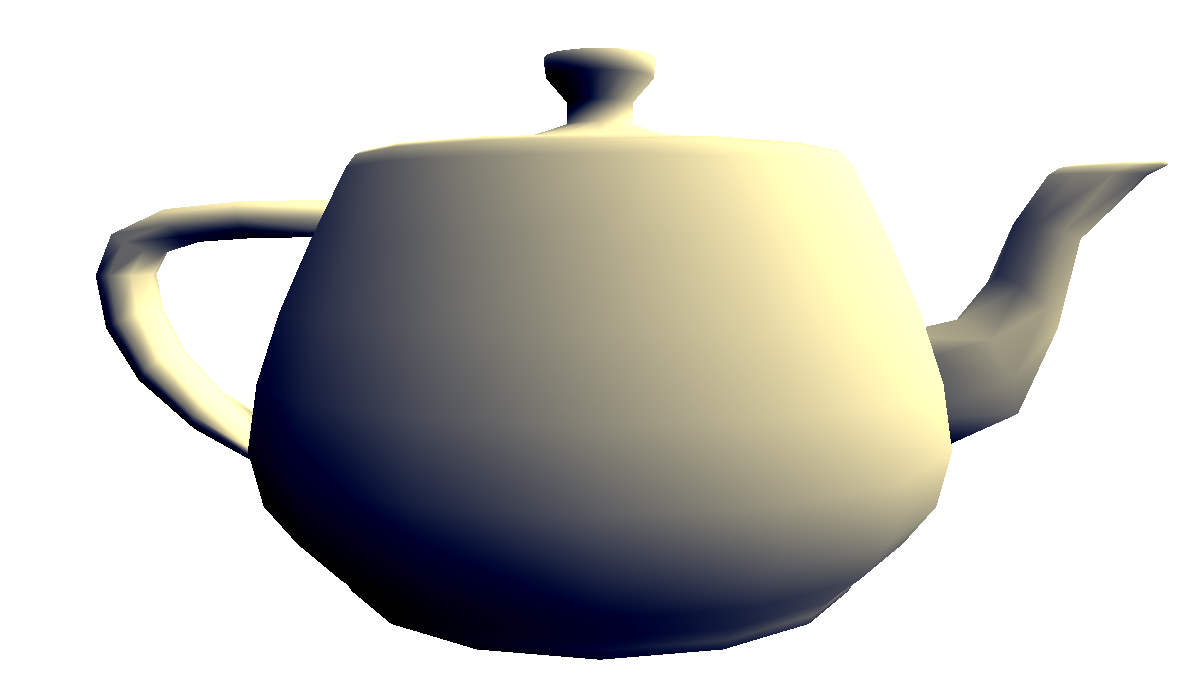
\includegraphics[width=8cm]{simple_s1_vert}\\
  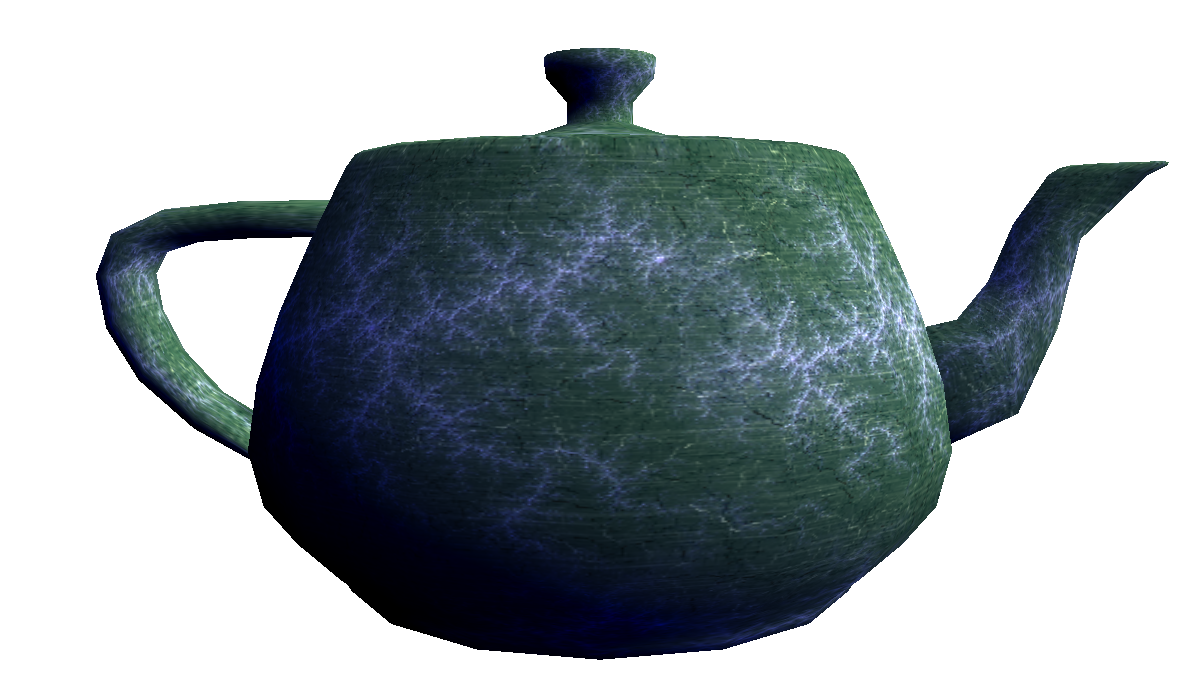
\includegraphics[width=8cm]{simple_s1_frag}
  \caption{Programm aus \ref{fig:simple_s1}}
  \small 1. nur per-Mesh-Anteil der Fragment-Farbe\\
  2. mit zusätzlich per-Vertex-Anteil\\
  3. vollständige Fragment-Farbe\\
  \label{fig:simple_s1_images}
\end{figure}

% Force figures to appear before section
\clearpage
\section{Code-Generator}

Der \emph{Code-Generator} übersetzt ein in der Zwischencoderepräsentation vorliegendes Programm in eine \emph{Zieldarstellung}.
Diese "`Darstellung"' kann wieder eine Hochsprache sein, prinzipiell kann ein Code-Generator aber auch Assembler-Quelltext oder eine
Binärcodierung ausgeben.

\subsection{Eingaben und Aufgaben}

Der \emph{Code-Generator} erhält als Eingabe eine Liste von Funktionsbeschreibungen.
Eine Funktionsbeschreibung besteht aus dem eindeutigen Bezeichner, einer Liste von Parametern (getrennt nach Ein- und Ausgabeparametern)
und einer Sequenz mit den eigentlichen Operationen. Eine Funktion aus der Liste ist als "`Eintrittsfunktion"' markiert.

\begin{figure}[h]
   \centering
  \includegraphics{ir_program}
  \caption{Zusammensetzung eines Programms in der Zwischencoderepräsentation}
  \label{fig:ir_program}
\end{figure}

Die Aufgaben des Code-Generators bestehen aus:
\begin{itemize}
\item Nötige Umformungen für die Zieldarstellung -- z.B. Schleifen ausrollen oder ``inlining'' von Funktionen.
\item Übertragung der Funktionsbeschreibungen in eine entsprechende Deklaration in der Zieldarstellung.
\item Übersetzung der Sequenzoperationen in die Zieldarstellung. 
\item Dabei Ressourcenallokation, wenn nötig (z.B. begrenzte Registerzahl in der Zieldarstellung).
\item Generierung von "`Schnittstellen-Anweisungen"' wie z.B. bei der Übergabe von Parametern an Funktionen
oder die Behandlung von Werten "`vor dem ersten Durchlauf, nach dem ersten Durchlauf"' wie sie bei Schleifen
auftreten.
\end{itemize}

\subsection{Generator für Cg}

In der vorliegenden Implementierung wurde als Zieldarstellung die Sprache Cg~(\cite{cgpaper}, \cite{cg_home}) gewählt.

Cg als Hochsprache kennt selbst Konstrukte wie Funktionen und Schleifen. Umformungen durch den Codegenerator
sind also nicht nötig.

Jede Funktion wird also direkt auf eine Cg-Funktion abgebildet.

Jedem Register der Zwischencoderepräsentation wird eine Variable zugeordnet -- eine Re\-gis\-ter\-al\-lo\-ka\-tion ist unnötig, diese wird später vom Cg-Compiler selbst vorgenommen.
"`Einfache"' Sequenzoperation (arithmetische Operationen u.ä.) lassen sich trivialerweise auf ein einzelnes Statement in Cg übertragen. 
Weiterhin werden die meisten eingebauten Funktionen und Attribute direkt von Cg unterstützt (Ausnahme ist das Matrix-Attribut \texttt{inverted}).

Kompliziertere Operationen -- Verzweigungen, Schleifen, Funktionsaufrufe -- resultieren in mehreren Statements, obwohl es sich bei dem
zusätzlichen "`Aufwand"' meist nur um Zuweisungen zwischen Variablen handelt, wie z.B. die Auswahl des Bedingungsregisters basierend zwischen
den Wert vor und nach dem ersten Schleifendurchlauf.

Die spezifizierte Sprache unterstützt Zeichenketten aus Unicode-Buchstaben und -Ziffern als Bezeichner;
Cg nur eine Untermenge von ASCII. Für die Ausgabe als Cg-Code werden Zeichen ausserhalb von ASCII in eine Darstellung in der von Cg akzeptieren
Zeichenmenge umgewandelt\footnote{Als Kodierung wurde Punycode~(\cite{rfc3492}) gewählt da dies die aus ASCII bestehenden Teile eines Bezeichners
gut lesbar lässt.}.

% Original-Schnipsel und Generator-Output

\newpage
\section{Optimierer}

\newcommand\OptSample[2]{
  \begin{figure}[!h]
    \centering
    \begin{minipage}{8cm}\lstinputlisting{s1source/opt_ex/#1.s1}\end{minipage}
    \begin{minipage}{10cm}\include{s1latex/opt_ex/#1_unopt}\end{minipage}
    \vspace{0.3em}
    \begin{minipage}{10cm}\include{s1latex/opt_ex/#1_opt}\end{minipage}
    \caption{#2.}
    \label{fig:ir_optex_#1}
  \end{figure}
}
\newcommand\OptSampleStacked[2]{
  \begin{figure}[!h]
    \centering
    \begin{minipage}{8cm}\lstinputlisting{s1source/opt_ex/#1.s1}\end{minipage}
    \begin{minipage}{10cm}\include{s1latex/opt_ex/#1_unopt}\end{minipage}\\
    \vspace{0.3em}
    \begin{minipage}{10cm}\include{s1latex/opt_ex/#1_opt}\end{minipage}
    \caption{#2.}
    \label{fig:ir_optex_#1}
  \end{figure}
}

Die Aufgabe eines \emph{Optimierers} ist es, ein gegebenes Programm so umzuschreiben, dass es zur Laufzeit
schnellstmöglich ausgeführt wird. Im allgemeinen erstrecken sich mögliche Optimierungen von Vereinfachungen,
wie ein Entfernen von unbenötigten Operationen und ein Berechnen von Ausdrücken zur Kompilierzeit,
bis hin zu komplexen Umsortierungen oder Zusammenfassung von Operationen, z.B. um ``multiply-add''-Operation
besser auszunutzen.

Ein Optimierer, der Redundanzen u.ä. entfernt, erlaubt als Nebeneffekt auch, dass die vorhergehenden Arbeitsschritte
eines Compilers -- im vorliegenden Compiler insbesondere der Splitter --
nicht selbst optimalen Zwischencode erzeugen müssen. Die Implementierung jener Arbeitsschritte kann damit
vereinfacht werden.

\subsection{Aufbau}

% Ein-, Ausgabe: Programme

Der Optimierer im vorliegenden Compiler nimmt als Eingabe ein komplettes Programm entgegen
und liefert als Ausgabe entsprechend auch ein komplettes Programm.

Das Arbeiten auf ganzen Programmen erlaubt es prinzipiell, funktionsübergreifende Optimierungen
vorzunehmen, von einem entfernen unbenötigter Funktionen über Inlining bis zu einem entfernen
einzelner, nicht benötigter Funktionsparameter.

Allerdings beschränken sich die implementierten, unten beschriebenen Optimierungen auf Sequenzen
von Operationen; diese Sequenzoptimierungen werden auf alle Funktionen eines Programms unabhängig
voneinander angewendet.

% mehrere Stufen
Die einzelnen Sequenzenoptimierungen werden nacheinander angewendet. Bei Bedarf kann eine
Optimierung mehrmals angewendet werden - z.B. kann das ``Constant Folding'' einen Ausführungszweig
einer Verzweigung auswählen; in diesem Fall wird ein erneutes ``Block Inlining'' veranlasst,
um die dadurch eingefügte Sequenzschachtelungsoperation zu vereinfachen.
% bei Bedarf mehrere Durchgänge -> z.B. erneutes BI when CF einen Branch o.ä. "geinlined" hat

\subsection{Block Inlining}

% 'entfernt' Block-Seqop.
Das \emph{Block Inlining} ersetzt alle Sequenzschachtelungsoperationen einer Sequenz durch
die in der eingeschachtelten Sequenz enthaltenen Operationen. Dabei werden die von den
Operationen verwendeten bzw. veränderten Register angepasst: Register, die einem importiertem
oder exportiertem Namen zugeordnet sind, werden durch ihre Gegenstücke in der umgebenden
Sequenz ersetzt. Andere Register werden umbenannt um Kollisionen zu vermeiden.

% v.a. "Hilfsschritt" für andere Opt.
Die vom Block Inlining vorgenommen Änderungen an einer Sequenz haben keine Auswirkungen auf das
Laufzeitverhalten des Programms. Dieser Optimierungsschritt dient vor allem als "`Hilfsschritt"',
um die Implementierungen anderer Optimierungsschritte zu vereinfachen: einerseits können
Sequenzschachtelungsoperationen als "`nicht vorhanden"' angenommen werden, andererseits kann
ein Inlining von Blöcken -- z.B. wegen der statischen Auswahl eines Verzweigungsblockes --
einfach vorgenommen werden, da die nötige "`Hauptarbeit"' später vom Block-Inlining-Schritt
vorgenommen wird.

Abbildung~\ref{fig:ir_optex_bi} vergleicht ein einfaches Programm vor und nach der Anwendung von Block Inlining.

\OptSampleStacked{bi}{Block Inlining: Quellcode, Zwischencoderepräsentation unoptimiert und optimiert}

\subsection{Constant Folding}

% Berechnung von konstanten Ausdrücken
% (Cast, Arithmetische, Logische, Unäre, Vergleichsop., Builtins, Arraylänge, Array getelem)
% Entfernung von Branches/Schleifen mit konst. Bedingung
\emph{Constant Folding} berechnet das Ergebnis einer Sequenzoperation zur Kompilierzeit
wenn alle Eingabeoperanden zur Kompilierzeit bekannte Konstanten sind. Berücksichtigt
werden Zuweisungs-, Cast-, arithmetische, logische, unäre und Vergleichsoperationen, alle eingebauten
Funktionen (mit Ausnahme von Texturfunktionen) sowie die Operationen "`Arraylänge"' und
"`Extraktion eines Arrayelements"'.
Weiterhin werden Verzweigungsoperationen, deren Bedingung ein konstanter Wert ist,
durch eine Schachtelung der entsprechenden Sequenz ersetzt (die andere Sequenz wird verworfen).
Auch Schleifenoperationen, deren Schleifenbedingung den konstanten Wert "`falsch"' besitzt,
werden verworfen.

% Fkt.weise: speichert für jedes Reg., ob konst., und wenn ja, dessen Wert;
% Op. auf Konstanten zur Kompilierzeit berechnet
In der Implementierung des Constant Folding wird eine Zuordnung zwischen Registern und konstanten
Werten verwendet; ist einem Register kein solcher Wert zugeordnet besitzt es keinen bekannten
konstanten Wert. Eine solche Zuordnung wird erstellt, wenn eine Operationen ein konstantes
Ergebnis hat. Dies sind zuvorderst Konstantenoperationen.
Bei Operationen, die einer der oben genannten Arten entsprechen, wird überprüft, ob alle Operanden
konstante Werte sind. Ist dies der Fall wird das Ergebnis der Operation vom Compiler berechnet
und die Operation durch eine einfache Konstantenoperation ersetzt.

% Zukunft: Funktionen mit rein konstanten Argumenten

Abbildung~\ref{fig:ir_optex_cf} vergleicht ein einfaches Programm vor und nach der Anwendung von Constant Folding.
Anzumerken ist, dass die Addition vom Compiler ausgerechnet und durch eine Konstantenoperation ersetzt
wird; die Konstantenoperationen der Quelloperanden bleiben jedoch erhalten - deren Entfernung ist
die Aufgabe der Dead Code Elimination, welche aber in diesem Beispiel nicht durchgeführt wurde.

\OptSampleStacked{cf}{Constant Folding: Quellcode, Zwischencoderepräsentation unoptimiert und optimiert}

\subsection{Dead Code Elimination}

\emph{Dead Code Elimination} entfernt unnötige Sequenzoperationen; eine Operation ist "`unnötig"',
wenn keines der von ihr geschriebenen Register jemals benutzt wird.

% entfernt Op., deren Ergebnis nie benutzt wird

In der Implementierung werden die Operationen einer Sequenz \emph{von hinten} betrachtet.
Es wird eine Menge von "`ausgelesenen"' Registern gespeichert. Bei jeder Operation wird
zunächst überprüft, ob wenigstens eins der Ausgaberegister ein solches "`ausgelesenes"'
Register ist. Ist dies nicht der Fall, wird die Operation verworfen. Andernfalls wird
die Operation beibehalten und alle ihre Eingaberegister als "`ausgelesen"' markiert.

Die Menge der "`ausgelesenen"' Register benötigt eine "`Saat"' von Registern, die als
immer ausgelesen angenommen werden (sonst würden alle Operationen einer Sequenz verworfen
werden). Dies sind immer die Ausgabeparameter der Funktion, die die Sequenz enthält.
Für Sequenzen, die z.B. in Verzweigungen eingeschachtelt sind, dient die Menge der
ausgelesenen Register der umgebenden Sequenz als Saat.

% Fkt.weise: iteriert Operationen rückwärts
% speichert zu jedem Reg., ob gelesen
% verwirft Op., deren Zielregister nie gelesen wurde
% verwirft Blöcke, bei denen kein "exportiertes" Register gelesen wurde
% verwirft Fkt.aufrufe, bei denen kein Ausgabereg. gelesen wurde
% benötigt "Saat-Register" (Ausgabeparameter)

Abbildung~\ref{fig:ir_optex_dce} vergleicht ein einfaches Programm vor und nach der Anwendung von Dead Code Elimination.
Dargestellt sind die Zwischencoderepräsentationen nach der Aufspaltung des Programms.
In den unoptimierten Programmen werden beide Ausgabeparameter sowohl in Vertex- als auch Fragmentprogramm
beschrieben, obwohl jeweils nur einer tatsächlich verwendet wird. Aus den optimierten Programmen wurde die jeweils unnötige
Zuweisung entfernt.

\OptSampleStacked{dce}{Dead Code Elimination: Quellcode, Zwischencoderepräsentation unoptimiert und optimiert;
Zwischencoderepräsentation nach Aufspaltung in Vertex- und Fragmentprogramme}

\section{Zusammenfassung}

Grundsätzlich folgt der Aufbau des Compilers der Standardarchitektur dafür; die Abweichnung ist der Verarbeitungsschritt der "`Auftrennung"' in mehrere
Programme.

Die Auftrennung nutzt dabei Eigenschaften von Graphikhardware aus, deren Aufbau auf den Ablauf des Echtzeit-3D-Renderings abgestimmt ist.
Speziell werden Operationen in der Vertex- statt Fragmentverarbeitung ausgeführt sofern das Ergebnis zur ursprünglichen Operation mathematisch äquivalent ist,
nachdem die von der Graphikhardware vorgenommen Interpolation von Ausgaben der Vertexverarbeitung angewendet wurde.

Auch hervorzuheben ist die verwendete Zwischencoderepräsentation, die als Übergabeformat zwischen allen Verarbeitungsschritten von der
semantischen Analyse bis zur Codegenerierung dient. Weiterhin ist sie darauf ausgerichtet, die Implementierung von Optimierungsschritten
möglichst zu vereinfachen.

\chapter{Ausblick}

% AST: nützlich, wenn FEs für anderen Sprachen, oder komplexer (Strukturen)
% Manuelles spezifizieren von per-Vertex Ops // keyword 'interpolate'

Die übersetzte Sprache ist eine zwar vergleichsweise einfache, aber trotzdem praktisch nutzbare
Shadingsprache, die es erlaubt, Shadingprogramme zu schreiben, ohne den Hardwareaufbau aus verschiedenen Funktionseinheiten
berücksichtigen zu müssen.

Der in Abschnitt~\ref{Auftrennung} beschriebene Auftrenner arbeitet konservativ in dem Sinne dass eine Operation nur in das Ausgabe-Vertex-Programm
"`verschoben"' wird wenn das Ergebnis mathematisch äquivalent zu einer Berechnung im Ausgabe-Fragment-Programm wäre.
Praktisch sollen aber manchmal bewusst Operationen durch eine per-Vertex-Berechnung approximiert werden (aus Geschwindigkeitsgründen
bei komplexen oder oftmals verwendeten Programmen). Die Sprache sollte deswegen noch um ein Schlüsselwort o.ä. erweitert werden
welches ein manuelles Bestimmen der Berechnungseinheit für eine Operation erlaubt.

Eine weitere Erweiterung, um das Erstellen von komplexeren Programmen zu vereinfachen, wäre das Hinzufügen von Verbundtypen zur Sprache.

Denkbar ist es auch, den Compiler so zu erweitern, dass Programme aus "`üblichen"' Shadingsprachen mit getrennten Vertex- und Fragmentprogrammen
-- wie Cg -- akzeptiert werden. Die Ausgabe des Compilers wären ein funktional äquivalente Vertex- und Fragment-Programme,
allerdings potentiell mit einer besseren Verteilung von Operationen auf Verarbeitungseinheiten.

Bei der Implementierung besteht praktisch das grösste Verbesserungspotential im Aufspalter. Die Behandlung von Funktionen ist relativ
kompliziert. Rekursiven Funktionen, aber auch Schleifen, werden nur im Fragment-Programm ausgeführt - dies stellt zwar ein korrektes
Ergebnis sicher, ist aber nicht in allen Fällen die optimale Lösung.

Der Compiler selbst nimmt in der vorliegenden Implementierung noch keine Optimierungsschritte vor. In Anbetracht der bewussten Ausrichtung
der Zwischencoderepräsentation auf möglichst einfache Optimierungen sowie die bei der Implementierung gemachten Annahmen (z.B. im Aufspalter) über das
Vorhandensein von Optimierungsschritten wäre es der nächste sinnvolle Schritte, diese Optimierungsschritte tatsächlich umzusetzen.

\cleardoublepage
\appendix

\printglossaries

\bibliography{thesis_de}
\addcontentsline{toc}{chapter}{Literatur}

\end{document}
